\documentclass[a4paper,twocolumn]{report}

% ---- pdflatex 基本 ----
\usepackage[T1]{fontenc}
\usepackage{lmodern}
\usepackage{microtype}

% ---- 箱(ascmac の代替)----
\usepackage{tcolorbox}
\tcbuselibrary{breakable}
\tcbuselibrary{skins}
% ascmac の itembox 代替:第1引数=tcolorboxのキー(任意),第2引数=タイトル(必須)
% 例)\begin{itembox}[halign title=left]{Problem} ... \end{itembox}
\newtcolorbox{itembox}[1]{%
  enhanced,breakable,
  colback=white,colframe=black,boxrule=0.4pt,arc=2pt,
  title={#1},
}


% ---- 以降はいつも通り ----
\usepackage{minted}
\usepackage{amsmath,amssymb,amsfonts,bm}
\usepackage{siunitx}
\usepackage{graphicx}
\usepackage[version=4]{mhchem}
\usepackage[colorlinks=true,bookmarks=true,bookmarksnumbered=true,
  linkcolor=cyan,urlcolor=blue,citecolor=blue]{hyperref}


\usepackage{color}
\definecolor{red}{rgb}{0.8,0.0,0.0}
\definecolor{gray}{rgb}{0.3,0.3,0.3}
%\usepackage{algorithm}
\usepackage{algorithmic}
%\usepackage{xltxtra}

\newcommand{\thetav}{\boldsymbol{\theta}}
\newcommand{\dv}{\boldsymbol{d}}
\newcommand{\rv}{\boldsymbol{r}}
\newcommand{\ev}{\boldsymbol{e}}
\newcommand{\Ysim}{\boldsymbol{Y}}
\newcommand{\Ysims}{{Y}}
\newcommand{\Yobs}{\boldsymbol{Y}_\mathrm{obs}}
\newcommand{\Yobss}{{Y}_\mathrm{obs}}
\newcommand{\Ysmsim}{\hat{Y}}
\newcommand{\Ysmobs}{\hat{Y}_\mathrm{obs}}


\newcommand{\Nsample}{N_\mathrm{s}}
\newcommand{\isample}{i_\mathrm{s}}
\newcommand{\Nthread}{N_\mathrm{th}}
\newcommand{\ithread}{i_\mathrm{th}}
\newcommand{\Nparticle}{N_\mathrm{p}}
\newcommand{\sobs}{s(\Yobs)}
\newcommand{\MES}{\mathrm{MES}}
\newcommand{\CDPP}{\mathrm{CDPP}}

%elements
\newcommand{\Hel}{\mathsf{H}}
\newcommand{\Oel}{\mathsf{O}}
\newcommand{\Cel}{\mathsf{C}}
\newcommand{\nel}{b}
\newcommand{\bv}{\boldsymbol{b}}
\newcommand{\nv}{\boldsymbol{n}}
\newcommand{\fv}{\boldsymbol{f}}
\newcommand{\Jv}{\boldsymbol{J}}
\newcommand{\xv}{\boldsymbol{x}}
\newcommand{\yv}{\boldsymbol{y}}

%inference
\newcommand{\epsilonv}{\boldsymbol{\epsilon}}
\newcommand{\pv}{\boldsymbol{p}}
\newcommand{\qv}{\boldsymbol{q}}

%gp etc
\newcommand{\Dp}{D} % # of parameters
\newcommand{\Mp}{M} % # of models
\newcommand{\Kp}{K} % # of layers


\newcommand{\mv}{\boldsymbol{m}}
\newcommand{\muv}{\boldsymbol{\mu}}
\newcommand{\partialv}{\boldsymbol{\partial}}
\newcommand{\omegav}{\boldsymbol{\omega}}
\newcommand{\av}{\boldsymbol{a}}
\newcommand{\uv}{\boldsymbol{u}}
\newcommand{\vv}{\boldsymbol{v}}
\newcommand{\gv}{\boldsymbol{g}}
\newcommand{\tv}{\boldsymbol{t}}
\newcommand{\mva}{\boldsymbol{m}^\ast}
\newcommand{\Ng}{\mathcal{N}}
\newcommand{\zerov}{\boldsymbol{0}}


\newcommand{\Fv}{\boldsymbol{F}}
\newcommand{\zv}{\boldsymbol{z}}
\newcommand{\hv}{\boldsymbol{h}}
\newcommand{\evv}{\boldsymbol{e}}
\newcommand{\ntot}{n_\mathrm{tot}}
\newcommand{\lnntot}{q_\mathrm{tot}}
\newcommand{\lnnv}{\boldsymbol{q}}
\newcommand{\lambdav}{\boldsymbol{\lambda}}
\newcommand{\piv}{\boldsymbol{\pi}}
\newcommand{\Piv}{\boldsymbol{\Pi}}
\newcommand{\Lv}{\boldsymbol{L}}
\newcommand{\lambdatot}{\lambda_\mathrm{tot}}
\newcommand{\alphav}{\boldsymbol{\alpha}}
\newcommand{\betav}{\boldsymbol{\beta}}
\newcommand{\etav}{\boldsymbol{\eta}}
\newcommand{\nelements}{m}
\newcommand{\gtot}{g_\mathrm{tot}}


\newcommand{\Blam}{B_\nu}
\newcommand{\Ilam}{{\mathcal{I}_\nu}}
\newcommand{\Jlam}{{\mathcal{J}_\nu}}
\newcommand{\Jl}{{J_\nu}}
\newcommand{\Hl}{{H_\nu}}
\newcommand{\Kl}{{K_\nu}}
\newcommand{\JlVIS}{{J_{\nu}^\star}}
\newcommand{\HlVIS}{{H_{\nu}^\star}}
\newcommand{\KlVIS}{{K_{\nu}^\star}}
\newcommand{\Ilams}{{\mathcal{I}}}

\newcommand{\Fsum}{F_\mathrm{sum}}
\newcommand{\Fdif}{F_\mathrm{net}}
\newcommand{\dotFsum}{\dot{F}_\mathrm{sum}}
\newcommand{\dotFdif}{\dot{F}_\mathrm{net}}
\newcommand{\ddotFsum}{\ddot{F}_\mathrm{sum}}
\newcommand{\ddotFdif}{\ddot{F}_\mathrm{net}}

\newcommand{\Il}{I_\nu}
\newcommand{\Bl}{B_\nu}
\newcommand{\dBl}{\dot{B}_\nu}

\newcommand{\Jlu}{J_+}
\newcommand{\Hlu}{H_+}
\newcommand{\Jld}{J_-}
\newcommand{\Hld}{H_-}
\newcommand{\dHlu}{\dot{H}_+}
\newcommand{\dHld}{\dot{H}_-}
\newcommand{\Fnet}{F_\mathrm{net}}
\newcommand{\dFsum}{\dot{F}_\mathrm{sum}}
\newcommand{\ddFsum}{\ddot{F}_\mathrm{sum}}
\newcommand{\dFnet}{\dot{F}_\mathrm{net}}
\newcommand{\Bv}{\boldsymbol{\mathcal{B}}}
\newcommand{\Gv}{\boldsymbol{G}}
\newcommand{\Gaa}{\mathcal{G}_{11}}
\newcommand{\Gab}{\mathcal{G}_{12}}
\newcommand{\Gba}{\mathcal{G}_{21}}
\newcommand{\Gbb}{\mathcal{G}_{22}}
\newcommand{\Gcross}{\mathcal{G}_{\times}}

%opacity
\newcommand{\Ncut}{M}
\newcommand{\nulc}{\hat{\nu}} %line center
\newcommand{\nulcl}{\nulc_{m,l}} %line center
\newcommand{\numatrix}{\hat{N}} %nu-matrix
\newcommand{\ntexp}{{\mathsf{n}}} %temperature exponent
\newcommand{\gw}{{\mathsf{g}}} %statistical weight

%clouds
\newcommand{\Kzz}{K_{zz}}
\newcommand{\fsed}{f_\mathrm{sed}}
\newcommand{\cond}{{\mathsf{c}}}
\newcommand{\total}{{\mathsf{tot}}}
\newcommand{\vapor}{{\mathsf{v}}}

\setlength{\textwidth}{460pt}
\setlength{\voffset}{0cm}
\setlength{\topmargin}{0.0cm}
\setlength{\headheight}{0.0cm}
\setlength{\headsep}{1cm}
\setlength{\oddsidemargin}{0.0cm}
\setlength{\evensidemargin}{0.0cm}
\begin{document}
\title{Inferring Exoplanets}
\author{Hajime Kawahara}
\maketitle

\tableofcontents

\chapter{Introduction}
Items marked with $\ast$ in each chapter are undergraduate review; in class we will only give a brief recap.
Sections marked with $\dagger$ contain detailed discussions and derivations. We will generally skip these; please read them if you have time. $\clubsuit$ indicates hints for calculations.
Items marked with $\ddagger$ are somewhat tangential to the main topic or provide additional material.


\section{Quantities$\,^\ast$}
Symbols for solar systems are as follows. $\odot$: Sun, $J$: Jupiter, $\oplus$: Earth
$R_x$ indicates th radis of $x$, $M_x$ is its $x$.

\subsection*{Lengths and Angles}
The radii of the solar systems
\begin{itemize}
    \item $R_\odot = 7 \times 10^5$ km
    \item $R_J = R_\odot/10$
    \item $R_\oplus = R_J/10 = R_\odot/100$
\end{itemize}
and the Schwarzschild radius of the Sun is given by
\begin{itemize}
   \item $r_g = 2 G M_\odot/c^2$ = 3 km.
\end{itemize}
However, it is useful to remember the following relation,
\begin{itemize}
    \item $\displaystyle{\frac{r_g}{2 \, \mathrm{au}}} = 10^{-8}$.
\end{itemize}
The solar radius is 1/100 of 1 au,
\begin{itemize}
    \item $\displaystyle{\frac{2 R_\odot}{1 \, \mathrm{au}}} = 10^{-2}$.
\end{itemize}
The distance to the nearest star is approximately 1 pc. The facts for the angle of $1^{\prime \prime}$: 
\begin{itemize}
    \item $1^{\prime\prime} = 5 \times 10^{-6}$ radian
    \item $\displaystyle{\frac{1 \mathrm{au}}{1 \mathrm{pc}}} = 1^{\prime\prime}$ \\
    \item typical seeing $\sim 1^{\prime\prime}$
    \item the apparent diamter of the moon $\sim 30^{\prime}$
\end{itemize}

\subsection*{Weight}

\begin{itemize}
    \item $M_\odot = 2 \times 10^{33}$ g
    \item $M_J = M_\odot/1000$
    \item $M_\oplus = M_J/300$
\end{itemize}


\chapter{Motion of A Planet}\label{ch:motion}
We consider quantities related to planetary motion as observable properties of exoplanets. Two such observables are the radial velocity curve, which measures the stellar motion along the line of sight induced by the planet, and astrometry, which traces the stellar motion projected on the celestial sphere.

\section{Two-Body Problem$^\ast$ \label{ss:twobody}}

We examine the motion and orbit of the planet–star system. Treating both the planet and the star as point masses ($m_1$, $m_2$) with positions ${\boldsymbol{r_1}},{\boldsymbol{ r_2}}$, and assuming that the only force acting between them is gravity, the system reduces to the two-body problem, which can be solved analytically. Defining ${\boldsymbol{ r}} \equiv {\boldsymbol{r_2}} - {\boldsymbol{ r_1}}$ as in Fig.~\ref{fig:zahyou}, we introduce a polar coordinate system in the orbital plane with basis vectors ${\bf e}_r=(\cos{\theta}, \sin{\theta})^\top$ and ${\bf e}_\theta=(-\sin{\theta}, \cos{\theta})^\top$. Then ${\bf r} = r {\bf e}_r$, and with $\dot{{\bf e}}_r=\dot{\theta} (-\sin{\theta}, \cos{\theta})^T = \dot{\theta} {\bf e}_\theta $ and $\dot{{\bf e}}_\theta=\dot{\theta}(-\cos{\theta}, -\sin{\theta})^T = - \dot{\theta} \,\dot{{\bf e}}_r$, we obtain
\begin{align}
\label{eq:speconv1}
\dot{\bf r} = \frac{d}{dt}{r {\bf e}_r} = \dot{r} {\bf e}_r + r \dot{{\bf e}}_r = \dot{r} {\bf e}_r + r \dot{\theta} {\bf e}_\theta \\
\ddot{\bf r} = (\ddot{r} - r \dot{\theta}^2 ) {\bf e}_r + \left[ \frac{1}{r} \frac{d}{dt} (r^2 \dot{\theta} ) \right] {\bf e}_\theta .
\end{align}

Because $\boldsymbol{r_1}=-m_2/(m_1+m_2) \, \rv, \, \boldsymbol{r_2}= m_1/(m_1 + m_2) \,\rv$, the Lagrangian, with the barycenter at the origin and using the reduced mass $\mu = (m_1^{-1} + m_2^{-1})^{-1}$, is
\begin{align}
L &= T - U = \frac{m_1}{2} |\dot{\boldsymbol{r_1}}|^2 + \frac{m_2}{2} |\dot{\boldsymbol{r_2}}|^2 + G \frac{m_1 m_2}{r} \nonumber \\
&= \frac{\mu}{2} [ \dot{r}^2 + (r \dot{\theta})^2 ] + G \frac{m_1 m_2}{r}.
\end{align}

\begin{figure}[]
 \begin{center}
	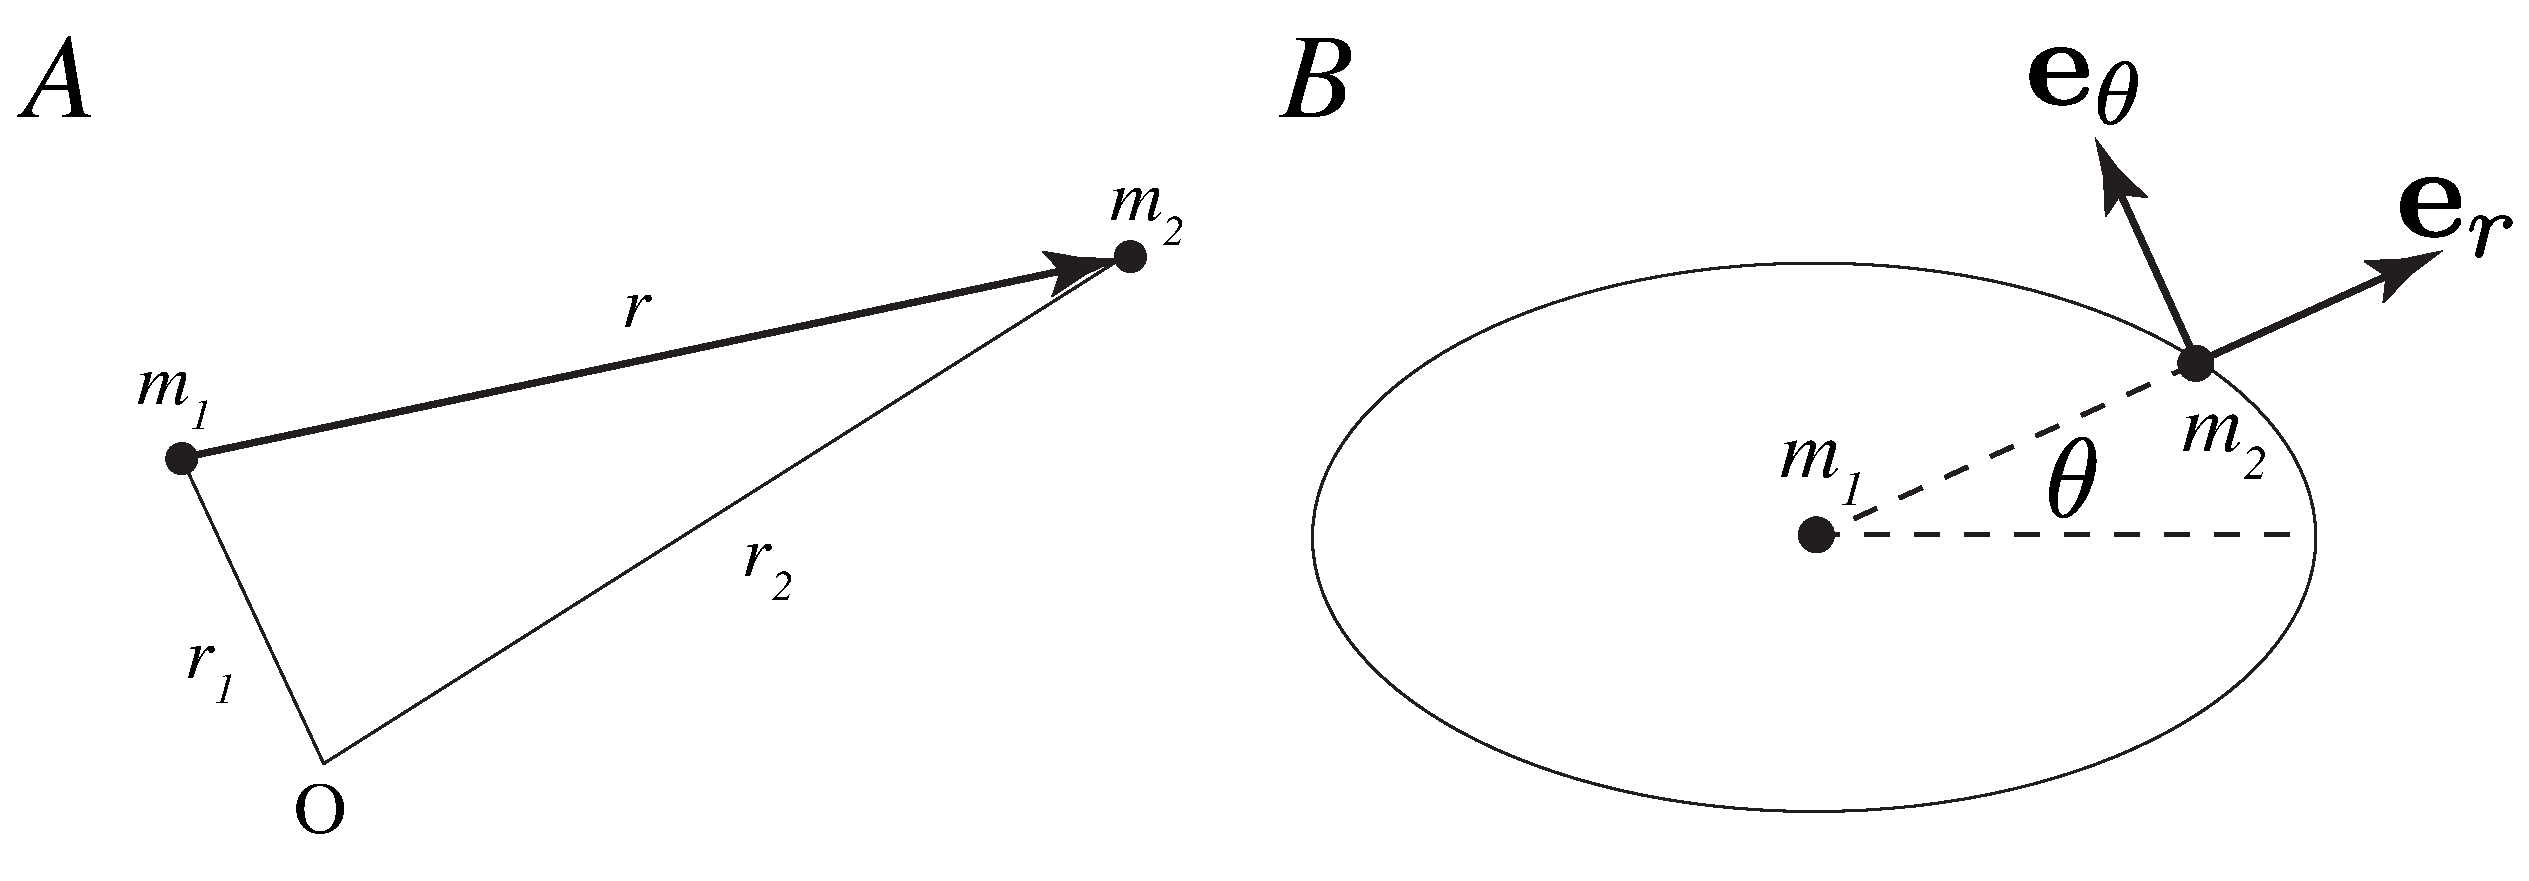
\includegraphics[width=\linewidth]{fig/zahyou.eps}
\end{center}
	\caption{Coordinate system}
	\label{fig:zahyou}
\end{figure} 


\color{red}
\begin{itembox}{Problem}
\footnotesize
\color{gray}
Derive 
\begin{align}
\label{eq:eqrad}
 \ddot{r} - r \dot{\theta}^2 = - \frac{G (m_1+m_2)}{r^2}
\end{align}
and $\dot{\bf h} =  0$ from the Lagrange equations
\begin{align}
\frac{d}{dt} \left( \frac{\partial L}{\partial \dot{r}}\right) - \frac{\partial L}{\partial r} = 0, \,\,\,
\frac{d}{dt} \left( \frac{\partial L}{\partial \dot{\theta}}\right) - \frac{\partial L}{\partial \theta} &= 0, 
\end{align}
where
$
{\bf h} \equiv {\bf r} \times \dot{\bf r} 
$
is the angular momentum vector. That is, the orbital angular momentum vector ${\bf h}$ is a conserved quantity in the two-body problem. This means that the point mass is constrained to move on the plane orthogonal to ${\bf h}$ (the orbital plane).
\end{itembox}
\color{black}

Transforming the variables in Eq.~(\ref{eq:eqrad}), let $u \equiv 1/r$. Using $h u^2 = \dot{\theta}$ and $\dfrac{d r}{d t} = \dfrac{d r}{d \theta} h u^2 = - h \dfrac{d u}{d \theta}$, we obtain
\begin{align}
\frac{d^2 u}{d \theta^2} + u = \frac{G (m_1 + m_2)}{h^2}
\end{align}
This is a nonhomogeneous second-order differential equation, whose homogeneous solution can be written as
\begin{align}
u_h = c_1 \cos{\theta} + c_2 \sin{\theta} = C_1 \cos{(\theta - C_2)} .
\end{align}
The nonhomogeneous solution is clearly
\begin{align}
u_i = \frac{G (m_1 + m_2)}{h^2} ,
\end{align}
and the general solution is the sum of these. Factoring out $G (m_1 + m_2)/h^2$ and introducing integration constants $e$ and $\omega$, the general solution can be written as
\begin{align}
u = \frac{G (m_1 + m_2)}{h^2} [ 1 + e \cos{(\theta - \omega)}] .
\end{align}
Returning to $r=1/u$, we obtain
\begin{align}
\label{eq:eqkep}
r = \frac{h^2}{G (m_1 + m_2)} \frac{1}{ 1 + e \cos{(\theta - \omega)}} .
\end{align}

Now, let us consider an ellipse as in Fig.~\ref{fig:ellip}. For an ellipse,
\begin{align}
\label{eq:rellp}
r + r^\prime = 2 a
\end{align}
holds. From the coordinates, we have
\begin{align}
\label{eq:rellp2}
(r^\prime)^2 &= (x_p + 2 e a )^2 + y_p^2 \nonumber \\
&= (r \cos{\theta} + 2 e a )^2 + (r \sin{\theta})^2 ,
\end{align}
and eliminating $r^\prime$ from Eqs.~(\ref{eq:rellp},\ref{eq:rellp2}), we obtain the conic equation of the ellipse
\begin{align}
\label{eq:conic_orig}
r = \frac{a (1-e^2)}{ 1 + e \cos{\theta}} .
\end{align}


\begin{figure}[]
 \begin{center}
	\includegraphics[bb=0 0 695 428,width=1.0\linewidth]{fig/ellip.png}
% \includegraphics[bb=0 0 474 461,width=1.0\linewidth]{fig/orbele.png}
\end{center}
	\caption{Ellipse.}
	\label{fig:ellip}
\end{figure} 

Defining the semi-major axis $a$, the semi-minor axis $b$, and the true anomaly $f$ as
\begin{align}
\label{eq:defkeppar1}
\frac{h^2}{G (m_1 + m_2)} &= a (1 - e^2) \\
\label{eq:defkeppar2}
b^2 &= a^2 (1 - e^2) \\
\label{eq:defkeppar3}
f &\equiv \theta - \omega ,
\end{align}
Eq.~(\ref{eq:eqkep}) takes the form of the conic equation
\begin{align}
\label{eq:conic_kepler}
r = \frac{a (1-e^2)}{ 1 + e \cos{f}} ,
\end{align}
which confirms that the solution of the two-body problem is an ellipse (with $0 \le e < 1$). The true anomaly $f$ corresponds to the angle of the star–planet system measured from the periastron (the point closest to the star, analogous to the solar periastron). The quantity $\omega$ is called the argument of periastron and represents a counterclockwise rotation of the ellipse described by the conic equation (\ref{eq:conic_orig}) by an angle $\omega$.

Since $\dot{A}$ is constant, the area of the ellipse can be written as
\begin{align}
A = \pi a b = \frac{h}{2} P ,
\end{align}
where $P$ is the orbital period. Rearranging this expression, we obtain
\begin{align}
\label{eq:kep3}
P^2 = \frac{4 \pi^2}{G (m_1+m_2)} a^3 ,
\end{align}
which shows that the square of the orbital period is inversely proportional to the total mass and proportional to the cube of the semi-major axis (Kepler’s third law). In the case of a circular orbit, the orbital angular velocity is given by $1/\sqrt{G (m_1+m_2) a}$. Eliminating $G$ using Eq.~(\ref{eq:defkeppar1}), we also obtain an expression in terms of angular momentum,
\begin{align}
\label{eq:kep3_1}
P = \frac{2 \pi a^2 \sqrt{1-e^2}}{h} .
\end{align}

\begin{figure}[]
 \begin{center}
%	\includegraphics[bb=0 0 695 428,width=1.0\linewidth]{fig/ellip.png}
 \includegraphics[bb=0 0 474 461,width=1.0\linewidth]{fig/orbele.png}
\end{center}
	\caption{Coordinate system.}
	\label{fig:ellip}
\end{figure} 

The mean motion is defined by
\begin{align}
    n \equiv \frac{2 \pi}{P}.
\end{align}
From equation (\ref{eq:kep3_1}), we can also express the mean motion as
\begin{align}
\label{eq:mean_motion}
    n = \frac{h}{a^2 \sqrt{1-e^2}}.
\end{align}


\section{Two-body problem in three-dimensional space \label{ss:threedtwobody}}

In the previous chapter, we considered two-body motion on a two-dimensional plane. In reality, celestial bodies exist in three-dimensional space from the perspective of an observer, so the orbit must be rotated into 3D. The orbital inclination $i$, which represents the tilt relative to the observer, and the longitude of the ascending node $\Omega$, which specifies the azimuthal direction, are introduced. By specifying the six parameters $a, e, \omega, f, i, \Omega$, the orbit of the two-body problem in three-dimensional space is uniquely determined.

Let us represent these rotations using rotation matrices. First, we take the reference ellipse to be that described by the conic equation (\ref{eq:conic_orig}) and shown in Fig.~\ref{fig:ellip}. The $z$-axis is taken perpendicular to the plane of the page.
\begin{itemize}
\item (1) Rotating the conic equation (\ref{eq:conic_orig}) counterclockwise about the $z$-axis by $\omega$ gives the ellipse of the two-body problem, Eq.~(\ref{eq:conic_kepler}).
\item (2) Next, rotating counterclockwise about the $x$-axis by $i$ tilts the orbital plane by $i$ with respect to the celestial sphere. 
\item (3) Finally, a remaining degree of freedom corresponds to rotation about the $z$-axis by $\Omega$, namely the azimuthal rotation on the celestial sphere.
\end{itemize}

Applying these rotation matrices in sequence to the vector representing the ellipse $\rv = (r \cos{\theta}, r \sin{\theta},0)$, we first obtain (1):

% ---- 1. position in the orbital plane ---------------------------------
\begin{align}
\rv &=
\begin{pmatrix}
r\cos\theta\\
r\sin\theta\\
0
\end{pmatrix}
=
\begin{pmatrix}
r\cos\!\bigl(f+\omega\bigr)\\
r\sin\!\bigl(f+\omega\bigr)\\
0
\end{pmatrix}
.
\end{align}
Next, (2) is 
% ---- 2. rotation by the inclination i (about the x-axis) --------------
\begin{align}
\rv^\prime &=
\begin{pmatrix}
1 & 0        & 0\\
0 & \cos i   & -\sin i\\
0 & \sin i   &  \cos i
\end{pmatrix}
\rv \\
&=
\begin{pmatrix}
r\cos\!\bigl(f+\omega\bigr)\\
r\sin\!\bigl(f+\omega\bigr)\cos i\\
r\sin\!\bigl(f+\omega\bigr)\sin i
\end{pmatrix}
.
\end{align}

% ---- 3. rotation by the longitude of ascending node Ω (about the z-axis)
Lastly, we obtain the trajectory in the three-dimensional space $(X,Y,Z)$ from (3):  
\begin{align}
\rv^{\prime\prime} &=
\begin{pmatrix}
\cos\Omega & -\sin\Omega & 0\\
\sin\Omega &  \cos\Omega & 0\\
0          &  0          & 1
\end{pmatrix}
\rv^\prime \\
&=
\begin{pmatrix}
r\cos\!\bigl(f+\omega\bigr)\cos\Omega
 - r\sin\!\bigl(f+\omega\bigr)\cos i\,\sin\Omega\\[4pt]
r\cos\!\bigl(f+\omega\bigr)\sin\Omega
 + r\sin\!\bigl(f+\omega\bigr)\cos i\,\cos\Omega\\[4pt]
r\sin\!\bigl(f+\omega\bigr)\sin i
\end{pmatrix}
\\
\label{eq:threed}
&\equiv
\begin{pmatrix}
X\\[2pt] Y\\[2pt] Z
\end{pmatrix}.
\end{align}

\section{Two-body problem as a function of time}

The solution to the two-body problem has so far been expressed as a function of the true anomaly $f$, namely $r = r(f)$. However, in actual observations, the two-body problem is always observed as a function of time. We therefore consider how to obtain the time-dependent expression $r = r(t)$.

The approach is as follows. First,
\begin{align}
v^2 &= \dot{\rv} \cdot \dot{\rv}
= (\dot{r} {\ev}_r + r \dot{f} {\ev}_\theta) \cdot (\dot{r} {\ev}_r + r \dot{f} {\ev}_\theta) \nonumber \\
\label{eq:v2_1}
&= \dot{r}^2 + r^2 \dot{f}^2 \\
\label{eq:v2_2}
&= \dot{r}^2 + \frac{h^2}{r^2} ,
\end{align}
where we used $h = r^2 \dot{f}$. Then,
\begin{itemize}
\item (1) Express $v^2$ in terms of $f$ by transforming $r$ and $\dot{r}$ in Eq.~(\ref{eq:v2_2}), giving $v^2(f)$.
\item (2) Transform $v^2(f)$ into $v^2(r)$ using the conic equation.
\item (3) Equating $v^2 = \dot{r}^2 + h^2/r^2$, derive an equation for $r$ and $\dot{r}$, namely a differential equation for $r$ with respect to time.
\end{itemize}

For step (1), the transformation from $r$ to $f$ can be made using the conic equation (\ref{eq:conic_kepler}). To express $\dot{r}$ in terms of $f$, we use
\begin{align}
\label{eq:dotr}
\dot{r} &= \frac{h}{a(1-e^{2})} \, e\sin f .
\end{align}

\begin{itembox}{$\clubsuit$ Derivation of Equation (\ref{eq:dotr})}
\footnotesize
\color{gray}
\begin{align}
    \dot r
  &=\frac{df}{dt}
   \,\frac{d}{df}\!
     \left(
       \frac{a(1-e^{2})}{1+e\cos f}
     \right)
  =\dot f\,
    \frac{a(1-e^{2})\,e\sin f}{\bigl(1+e\cos f\bigr)^{2}}
    \nonumber \\
    &= \dot{f} \frac{a (1-e^2)}{1 + e \cos{f}} \frac{e \sin{f}}{1 + e \cos{f}} = r \dot{f} \frac{e \sin{f}}{1 + e \cos{f}} \nonumber\\
&= \frac{h}{r} \frac{e \sin{f}}{1 + e \cos{f}}
= \frac{h}{a(1-e^{2})}\,e\sin f
\end{align}
\end{itembox}

Then, we obtain
\begin{align}
    v^2 &= \dot{r}^2 + (r \dot{f})^2 = \dot{r}^2 + \frac{h^2}{r^2} \nonumber \\
    &= \frac{h^2}{a^2(1-e^2)^2} [2 (1 + e\cos{f}) + e^2 - 1 ] = v^2(f).
\end{align}


Next, step (2), where $v^2(f)$ is transformed back into a function of $r$ using the conic equation, gives
\begin{align}
v^2(r) &= \frac{h^2}{a (1 - e^2)} \left( \frac{2}{r} - \frac{1}{a} \right) .
\end{align}
From step (3), we obtain the time differential equation for $r$:
\begin{align}
\label{eq:rde}
\dot{r}^2 - \frac{h^2}{a (1-e^2)} \left( \frac{2}{r} - \frac{1}{a} \right) + \frac{h^2}{r^2} = 0 .
\end{align}
This equation cannot be solved directly. Therefore, we introduce the eccentric anomaly $E$:
\begin{align}
\label{eq:eanomaly}
r = a (1 - e \cos{E}) .
\end{align}
Using this $E$, we transform the differential equation (\ref{eq:rde}) into a differential equation in terms of $E$ and $\dot{E}$:
\begin{align}
\label{eq:dee}
\dot{E} = \frac{n}{1 - e \cos{E}} .
\end{align}
Although introduced somewhat ad hoc, the solution is given by
\begin{align}
E - e \sin{E} = n (t -t_0) ,
\end{align}
and one can verify Eq.~(\ref{eq:dee}) by differentiation. Here, defining the mean anomaly $M$ as a proxy for the time variable,
\begin{align}
M \equiv n (t - t_0),
\end{align}
we obtain
\begin{align}
\label{eq:dee_sol_M}
f(E) = E - e \sin{E} - M = 0 ,
\end{align}
whose solution yields $E$.

\begin{itembox}{$\clubsuit$ Derivation of Equation (\ref{eq:dee})}
\footnotesize
\color{gray}
\begin{align}
  \frac{2}{r}-\frac{1}{a}
    &=\frac{1}{a}\!\left(\frac{2}{1-e\cos E}-1\right)     \nonumber \\
    &=\frac{1}{a}\,\frac{1+e\cos E}{1-e\cos E}
      \;=\;
      \frac{1}{a}\,
      \frac{1-e^{2}\cos^{2}E}{(1-e\cos E)^{2}}\;.
\end{align}

\begin{align}
 &\frac{h^{2}}{r^{2}}
 -\frac{h^{2}}{a^{2}(1-e^{2})}\!
  \left(\frac{2}{r}-\frac{1}{a}\right) \nonumber \\
 &= \frac{h^{2}}{a^{2}(1-e\cos E)^{2}}
    -\frac{h^{2}(1-e^{2})}{a^{2}(1-e\cos E)^{2}(1-e^{2})} \nonumber \\
 &=\frac{h^{2}(1-e^{2})}{a^{2}(1-e\cos E)^{2}(1-e^{2})} -\frac{h^{2}(1-e^{2}\cos^{2}E)}{a^{2}(1-e\cos E)^{2}(1-e^{2})}\nonumber \\
 &= -\frac{h^{2}e^{2}\bigl(1-\cos^{2}E\bigr)}
        {a^{2}(1-e\cos E)^{2}(1-e^{2})}
\end{align}

\begin{align}
     \dot r &=\frac{dE}{dt}\,
         \frac{d}{dE}\bigl(a(1-e\cos E)\bigr)
     =\dot E\,a e\sin E \\
  \dot r^{2}
    &=\dot E^{2}\,a^{2}e^{2}\sin^{2}E
\end{align}

From these equations, we obtain
\begin{align}
    \dot E^{2}\,a^{2}e^{2}\bigl(1-\cos^{2}E\bigr)
  =
  \frac{h^{2}\,e^{2}\bigl(1-\cos^{2}E\bigr)}
       {a^{2}(1-e\cos E)^{2}(1-e^{2})},
\end{align}
that is,
\begin{align}
    \dot E^{2}
   =\frac{h^{2}}
          {a^{4}(1-e\cos E)^{2}(1-e^{2})}
\end{align}
Assuming $\dot{E} > 0$, we obtain
\begin{align}
    \dot E
 &=\frac{h}{a^{2}\sqrt{1-e^{2}}\,(1-e\cos E)} \\
 & = \frac{n}{1 - e \cos{E}}.
\end{align}

We used the representation of the mean motion (\ref{eq:mean_motion}).
\end{itembox}
Furthermore, the relationship between $E$ and $f$ can be derived from Eq.~(\ref{eq:eanomaly}) and the conic equation of the two-body problem (\ref{eq:conic_kepler}):
\begin{align}
\label{eq:Efrel}
\cos{f} = \frac{\cos{E} - e}{1 - e \cos{E}} .
\end{align}

Thus, once the period $P$ and the offset $t_0$ are known, the mean anomaly $M$ can be calculated from the time $t$. By solving Eq.~(\ref{eq:dee_sol_M}) numerically, one obtains $E$, and then the true anomaly $f$ can be determined from Eq.~(\ref{eq:Efrel}).\\

\subsubsection{Solving Eq.~(\ref{eq:dee_sol_M}) using the Newton–Raphson method}

The nonlinear equation $f(E)=0$ must be solved numerically. One method for doing so is the Newton–Raphson method. As illustrated in Fig.~\ref{fig:newton_raphson}, the procedure begins with an initial guess $E_1$, then determines the tangent line to $f(E)$ at $E_1$, and finds analytically the intersection of this line with the $E$-axis, which is taken as $E_2$. Repeating this procedure $n$ times yields successive approximations. At the $i$-th step, the tangent line (i.e., the first-order Taylor expansion of $f(E)$ about $E_i$) is
\begin{align}
\label{eq:nrm}
y = f(E_i) + f^\prime(E_i) (E - E_i) ,
\end{align}
and therefore,
\begin{align}
\label{eq:update_newton}
E_{i+1} &= E_i + \Delta E_i \\
\Delta E_i &\equiv - \frac{f(E_i)}{f^\prime(E_i)} .
\end{align}
Here, $\Delta E_i$ is called the update term at the $i$-th iteration\footnote{This can also be viewed simply as updating the solution using the first-order Taylor approximation of $f(E)$,
\begin{align}
\label{eq:nrm_f}
f(E) \approx f(E_i) + f^\prime(E_i) (E - E_i) = 0 ,
\end{align}
taking $E_{i+1}$ as the solution, and repeating the procedure.}. This iteration is repeated until the convergence criterion $|E_{i+1} - E_i| < \epsilon$ is satisfied, where $\epsilon$ is the tolerance, and the resulting $E_i$ is taken as the approximate solution.

For the calculation in Eq.~(\ref{eq:nrm}), the derivative of $f$ is required. From Eq.~(\ref{eq:dee_sol_M}),
\begin{align}
f^\prime(E) = 1 - e \cos{E} .
\end{align}


\begin{figure}[]
 \begin{center}
 \includegraphics[width=1.0\linewidth]{fig/newton_raphthon.png}
\end{center}
	\caption{Newton-Raphson method.}
	\label{fig:newton_raphson}
\end{figure} 

\begin{itembox}{Newton's method as 2nd-order optimization$^\dagger$}
\footnotesize
\color{gray}
Consider the optimization problem of finding $x = x^\ast$ that minimizes a cost function $Q(x)$:
\begin{equation}
x^\ast = \mathrm{minimize}_{x} \,\, Q(x) .
\end{equation}
The stationary condition
$d Q(x)/d x = 0$
can be solved using the Newton–Raphson method. In this case, by setting
$f (x) = Q^\prime (x)$
and applying Eq.~(\ref{eq:update_newton}), the update rule becomes
\begin{align}
x_{i+1} &= x_i + \Delta x_i \\
\Delta x_i &\equiv - \frac{Q^\prime (x_i)}{Q^{\prime\prime}(x_i)} ,
\end{align}
which requires the second derivative of $Q(x)$. For this reason, it is called second-order optimization. In the context of optimization, the term ``Raphson'' is usually omitted, and it is simply called Newton's method.

In general, the multidimensional version of Newton's method can be formulated in the same way. From the multidimensional Taylor expansion,
\begin{align}
\fv(\xv) \approx \fv(\xv_i) + \Jv (\xv_i) (\xv - \xv_i) = \boldsymbol{0},
\end{align}
the solution $\xv$ becomes the next update point, leading to
\begin{align}
\xv_{i+1} &= \xv_{i} + \Delta \xv_i \\
\label{eq:second_newton}
\Delta \xv_i &\equiv - \Jv^{-1} (\xv_i) \fv(\xv_i) ,
\end{align}
where $\Jv (\xv_i)$ is the Jacobian at $\xv_i$.
\end{itembox}


\section{Radial velocity}\label{sec:rv}

The first detection of an exoplanet was achieved by measuring the variation in the stellar radial velocity induced by the planet’s orbital motion, observed through the Doppler shift of the stellar spectrum.

\begin{figure}[]
\begin{center}
\includegraphics[bb=0 0 648 537,width=1.0\linewidth]{fig/rvector.png}
\end{center}
\caption{Definition of the barycenter $o$ and each vector.\label{fig:rvector}}
\end{figure}

We now consider the radial velocity variation of a star caused by an orbiting planet. In the two-body case, the observed stellar radial velocity corresponds to the motion of the vector measured from the system barycenter. As shown in Fig.~\ref{fig:rvector}, let the planet be denoted by $p$, the star by $\star$, and their barycenter by $o$. The stellar and planetary masses are $M_\star$ and $M_p$, and their positions are ${\bf r}_\star$ and ${\bf r}_p$, respectively. The barycenter ${\bf r}_o$ of this system is given by
\begin{eqnarray}
{\bf r}_o = \frac{M_\star {\bf r}_\star+ M_p {\bf r}_p}{M_\star + M_p}
\label{eq:rbary}
\end{eqnarray}
The positions relative to the barycenter are defined as ${\bf \hat{r}}_\star = {\bf r}_\star - {\bf r}_o$, ${\bf \hat{r}}_p = {\bf r}_p - {\bf r}_o$, and the vector from the star to the planet as ${\bf \hat{r}} = {\bf \hat{r}}_p - {\bf \hat{r}}_\star$. Then,
\begin{align}
\label{eq:barycentsp}
M_\star {\bf \hat{r}}_\star + M_p {\bf \hat{r}}_p &= M_\star {\bf \hat{r}}_\star + M_p ({\bf \hat{r}}_\star + {\bf \hat{r}} ) = 0 ,
\end{align}
which gives
\begin{eqnarray}
\label{eq:relpossp}
{\bf \hat{r}}_\star = - \frac{M_p}{M_\star + M_p} {\bf \hat{r}} .
\end{eqnarray}

The position vector of the star as seen by the observer can then be expressed using the barycenter position vector ${\bf r}_o$:
\begin{eqnarray}
{\bf r}_\star = {\bf r}_o + {\bf \hat{r}}_\star .
\end{eqnarray}
Since the star moves in the opposite direction to the planet, let us take the line of sight along the negative $Z$-axis and, in order to preserve the counterclockwise orientation, set $\Omega = \pi$. In this case, the stellar radial velocity is given by the negative of the inner product of the time derivative with the unit vector ${\bf e}_Z$ in the $Z$ direction,
\begin{eqnarray}
\label{eq:vrsatare}
v_r = V_\mathrm{sys} - \dot{\hat{\bf r}}_\star \cdot {\bf e}_Z ,
\end{eqnarray}
where $V_\mathrm{sys} \equiv - \dot{{\bf r}}_o \cdot {\bf e}_Z $ is the systemic velocity of the entire system. From Eq.~(\ref{eq:relpossp}),
\begin{eqnarray}
\label{eq:vrsatare2}
v_r = V_\mathrm{sys} + \frac{M_p}{M_\star + M_p} \dot{\hat{\bf r}} \cdot {\bf e}_Z .
\end{eqnarray}
Here, ${\bf \hat{r}}$ corresponds to ${\bf r}$ in the two-body problem in the previous section, so the same formalism can be applied directly. Thus, $\dot{\hat{\bf r}}_\star \cdot {\bf e}_Z$ corresponds to the time derivative of the $Z$ component in the three-dimensional coordinate system, $\dot{Z}$. Using Eq.~(\ref{eq:threed}),
\begin{eqnarray}
\label{eq:vrsatare3}
v_r &=& V_\mathrm{sys} + \frac{M_p}{M_\star + M_p} \dot{Z} ,
\end{eqnarray}
with
\begin{align}
\dot{Z} &= \frac{d}{d t} \left[ r \sin{i} \sin{(f + \omega)} \right] \nonumber \\
&= \dot{r} \sin{i} \sin{(f + \omega)} + r \dot{f} \sin{i} \cos{(f + \omega)} .
\end{align}

Using Eq.~(\ref{eq:dotr}), $r \dot{f} = h/r$, and the conic equation (\ref{eq:conic_kepler}), we obtain
\begin{align}
\label{eq:vrsatare4}
&v_r =V_\mathrm{sys} + \frac{M_p}{M_\star + M_p} \frac{h \sin{i}}{a (1-e^2)} [ e \sin{f} \sin{(f+\omega)} \nonumber \\
&+ e \cos{f} \cos{(f+\omega)} + \cos{(f+\omega)} ] \\
&=V_\mathrm{sys} + \frac{M_p}{M_\star + M_p} \frac{h \sin{i}}{a (1-e^2)} \left[ \cos{(f+\omega)} + e \cos{\omega} \right] \nonumber \\
\end{align}

\begin{itembox}{$\clubsuit$}
\footnotesize
\color{gray}
$\sin{f} \sin{(f+\omega)} + \cos{f} \cos{(f+\omega)} = \cos{(-f)} \cos{(f+\omega)} - \sin{(-f)} \sin{(f+\omega)} = \cos{(-f + f + \omega)} = \cos{\omega}$
\end{itembox}

Alternatively, writing out $h$ explicitly, we obtain
\begin{align}
\label{eq:vrsatarefinal}
v_r &= V_\mathrm{sys} + K_\star \left[ \cos{(f+\omega)} + e \cos{\omega} \right] \\
\label{eq:vrKrv}
K_\star &\equiv \frac{M_p \sin{i}}{\sqrt{1 - e^2}} \sqrt{\frac{G}{(M_p + M_\star) a}} ,
\end{align}
which represents the radial velocity curve of the two-body problem. The order of magnitude of the radial velocity variation is
\begin{align}
K_\star &\sim 30 \mathrm{m/s} , \frac{M_p \sin{i}}{M_J}\left(\frac{M_\star}{M_\odot} \right)^{-1/2} \left(\frac{a}{\mathrm{au}} \right)^{-1/2} \\
&= 130 \mathrm{m/s} , \frac{M_p \sin{i}}{M_\oplus}\left(\frac{M_\star}{M_\odot} \right)^{-1/2} \left(\frac{a}{0.05 \mathrm{au}} \right)^{-1/2} \mbox{(HJ)} \nonumber \\
&= 0.1 \mathrm{m/s} , \frac{M_p \sin{i}}{M_\oplus}\left(\frac{M_\star}{M_\odot} \right)^{-1/2} \left(\frac{a}{\mathrm{au}} \right)^{-1/2} \mbox{(Earth)} \nonumber
\end{align}
The Doppler shift corresponding to this radial velocity variation is
\begin{align}
\frac{\Delta \lambda}{\lambda} &\sim \frac{K_\star}{c} \nonumber \\
& = 10^{-7} \frac{M_p \sin{i}}{M_J} \left(\frac{M_\star}{M_\odot} \right)^{-1/2} \left(\frac{a}{\mathrm{au}} \right)^{-1/2} .
\end{align}

Since the spectral resolution of current high-dispersion spectrographs is $R \sim 10^5$, it is important to boost the signal-to-noise ratio using many molecular absorption lines (and photon counts). In practice, stabilizing wavelength calibration with iodine cells or frequency combs is also crucial.

\begin{itembox}{$\clubsuit$}
%\tiny
\footnotesize
\color{gray}
\begin{align}
    K_\star &\sim \frac{M_p \sin{i}}{M_\odot}\left(\frac{M_\star}{M_\odot} \right)^{-1/2}  \sqrt{ \frac{G M_\odot}{a} } \nonumber \\
    &= \frac{M_p \sin{i}}{M_\odot}\left(\frac{M_\star}{M_\odot} \right)^{-1/2} \sqrt{ \frac{2 G M_\odot}{c^2}\frac{1}{2a} } \, c \nonumber \\
    &= \frac{M_J}{M_\odot} \frac{M_p \sin{i}}{M_J} \left(\frac{M_\star}{M_\odot} \right)^{-1/2} \sqrt{ \frac{r_g}{2  \mathrm{au}} \frac{\mathrm{au}}{a} }\, c \nonumber \\
    &= 10^{-7} c \frac{M_p \sin{i}}{M_J}  \left(\frac{M_\star}{M_\odot} \right)^{-1/2} \left(\frac{a}{\mathrm{au}} \right)^{-1/2} \nonumber \\
    &= 30 \mathrm{m/s} \, \frac{M_p \sin{i}}{M_J}\left(\frac{M_\star}{M_\odot} \right)^{-1/2} \left(\frac{a}{\mathrm{au}} \right)^{-1/2} \nonumber
\end{align}
\end{itembox}


\subsection*{Radial velocity curve as a function of time}

In actual observations, measurements are obtained as functions of time, so we would like to express the solution in terms of time. From the time $t$ and the orbital period, the mean anomaly $M$ can be determined. The eccentric anomaly $E$ is then obtained by numerically solving Eq.~(\ref{eq:dee_sol_M}). Using these, Eq.~(\ref{eq:vrsatarefinal}) can be rewritten numerically as a function of time.

Thus, the physical quantities that can be derived from the radial velocity curve are, from Eq.~(\ref{eq:vrsatarefinal}), $V_\mathrm{sys}, K_\star, e, \omega$. In addition, the orbital period $P$ and a phase parameter (the time offset) related to $f$ can also be estimated. Figure~\ref{fig:rvsim} shows several radial velocity curves and the corresponding elliptical orbits. According to Kepler’s second law, one can see that the radial velocity curve changes rapidly when the body approaches periastron.

\begin{figure}[]
\begin{center}
\includegraphics[width=\linewidth]{fig/rvsim.pdf}
\end{center}
\caption{Radial velocity curves (left) and corresponding orbits (right). The upper panels are for $\omega=\pi/6$, and the lower panels are for $\omega=\pi/2$. Line styles: black solid line for $e=0$, black dashed line for $e=0.5$, and gray solid line for $e=0.8$. The ellipses on the right correspond to orbits viewed from above when $i=\pi/2$. If the line of sight is taken from bottom to top, they correspond to the stellar orbit in the radial velocity curve, while if taken from top to bottom, they correspond to the planetary orbit. \label{fig:rvsim}}
\end{figure}

\begin{itembox}{Binary Mass Function$,^\dagger$}
%\tiny
\footnotesize
\color{gray}
Radial velocity analysis was originally developed for binary star systems before it was applied to star–planet systems. In this case, the approximation $M_p \ll M_\star$ does not hold. Rewriting Eq.~(\ref{eq:vrKrv}) with $\star \to 1$ and $p \to 2$, and using Kepler’s third law (\ref{eq:kep3}), we can separate the right-hand side into observable quantities and the left-hand side into physical parameters, giving
\begin{align}
\label{eq:bmfunc}
f \equiv \frac{M_2^3}{(M_1 + M_2)^2} \sin^3{i} = \frac{P K_1^3}{2 \pi G} (1 - e^2)^{3/2} .
\end{align}
Here, $f$ is a quantity that can be determined solely from the observed parameters of star 1’s radial velocity curve, $K_1$, $e$, and $P$, even in the general case of arbitrary mass ratios. This $f$ is called the binary mass function\index{Binary Mass Function@Binary Mass Function}.

Conversely, using a scaled form,
\begin{align}
\label{eq:semiamp2}
K_1 &= 29.8 , [\mathrm{km/s}] \frac{\sin{i}}{\sqrt{1 - e^2}} \left( \frac{M_2}{M_1 + M_2} \right) \nonumber \\
&\times \left( \frac{M_1 + M_2}{M_\odot} \right)^{1/3} \left( \frac{P}{1 \mathrm{yr}} \right)^{1/3} ,
\end{align}
is useful for estimating the detectability in the case of binary systems. The value 29.8 km/s corresponds to the Earth’s orbital velocity.
\end{itembox}


\section{Astrometry}

The radial velocity variation makes use of the $\dot{Z}$ component of the three-dimensional Keplerian motion. Since astrometry is the method of measuring the position of a star on the celestial sphere, it makes use of the ($X,Y$) components of the motion. After correcting for proper motion and parallax, the position of the star due to two-body motion can be expressed as an observable angle,
\begin{align}
{\boldsymbol{\theta}} = \frac{\hat{\rv}_\star}{d} = - \frac{M_p}{M_\star + M_p} \frac{\hat{\rv}}{d} ,
\end{align}
which is a two-dimensional projection, where $d$ is the distance between the observer and the star. From Eq.~(\ref{eq:threed}), we have
\begin{align}
\theta_x &= - \frac{M_p}{M_\star + M_p} \frac{X}{d} = - \frac{M_p}{M_\star + M_p} \frac{r}{d} \nonumber\\
&\times [\cos \bigl(f+\omega\bigr)\cos\Omega
- \sin \bigl(f+\omega\bigr)\cos i \, \sin\Omega] \\
\theta_y &= - \frac{M_p}{M_\star + M_p} \frac{Y}{d} =- \frac{M_p}{M_\star + M_p}\frac{r}{d} \nonumber\\
&\times [ \cos \bigl(f+\omega\bigr) \sin\Omega 
+ \sin \bigl(f+\omega\bigr)\cos i \,\cos\Omega] .
\end{align}

This solution is invariant under the transformation ($i \to \pi - i$, $f \to 2 \pi - f$, $\omega \to 2 \pi - \omega$), which means that astrometry alone cannot distinguish whether the planet is approaching or receding.

\chapter{Inference of Motion}\label{ch:infer}

In Chapter~\ref{ch:motion}, we discussed physical models of observables related to the motion of exoplanets. All of these are one-dimensional time-series data. In this chapter, we focus on estimating the internal parameters—namely the physical properties of exoplanets—by combining physical and statistical models with one-dimensional time-series data.


By comparing observational data $\dv$ with a theoretical model $\fv$, one can address the following:
\begin{enumerate}
\item Determine whether a given theoretical model $\fv$ can explain the observational data.
\item Assuming that a theoretical model $\fv$ is correct, determine or estimate the parameters $\thetav$ included in that model based on the data $\dv$ ({\bf parameter estimation}).
\item When multiple models exist, determine which model better explains the observations $\dv$ ({\bf model selection}).
\end{enumerate}

Since model selection is considerably more involved, here we focus on parameter estimation.

As an example, let us consider the comparison between radial velocity observational data and a theoretical model. In this case, $\dv$ can be regarded as a vector consisting of the radial velocity data series, with each element $d_i$ associated with the corresponding time $t_i$, making it comparable to the theoretical model. The theoretical model is given by Eq.~(\ref{eq:vrsatarefinal}). The parameter vector is $\thetav = (V_\mathrm{sys}, K_\star, e, \omega, T_0, P)$.

\begin{itembox}{Radial velocity raw data $\dv$}
\footnotesize
\color{gray}
See \href{https://github.com/HajimeKawahara/class25}{https://github.com/HajimeKawahara/class25}
.
\end{itembox}

\section{Point estimation and optimization}

Parameter estimation that selects a single parameter vector $\thetav$ for a model $\fv(\thetav)$ by comparing it with data $\dv$ is called \underline{point estimation}. If the data contained no errors at all, we would simply need to find $\thetav$ such that
\begin{align}
\dv - \fv(\thetav) = \boldsymbol{0} .
\end{align}
However, in practice, observational data contain errors, and such a $\thetav$ usually cannot be found. Instead, we can write
\begin{align}
\dv = \fv(\thetav^\ast) + \epsilonv ,
\end{align}
which implies that the model $\fv$ is correct, that a “true” parameter $\thetav^\ast$ exists, and that the residual vector $\epsilonv$ originates solely from observational errors. To formulate the theory in a way that incorporates observational errors, we need a probabilistic model that generates these errors. For example, if $\epsilonv$ follows an independent zero-mean normal distribution,
\begin{align}
\epsilon_i \sim \mathcal{N}(0,\sigma) ,
\end{align}
we can write more compactly that the physical model $\fv(\thetav^\ast)$ is the mean of the probabilistic model:
\begin{align}
d_i \sim \mathcal{N} (f_i(\thetav^\ast), \sigma) .
\end{align}

From this discussion, it becomes clear that when we speak of comparing observational data with a theoretical model, the theoretical model must include not only $\fv$ but also a probabilistic model. Schematically,
\begin{itembox}{Empirically testable theoretical model}
Testable theory = Physical/Chemical model $+$ Probabilistic model
\end{itembox}

In practice, theoretical astronomy often overemphasizes the physical/chemical model while neglecting the probabilistic model, whereas observational astronomy tends to fix the physical/chemical model. Constructing probabilistic models has historically been computationally demanding and thus difficult to handle until recently. However, advances in computing power and Bayesian statistical methods now allow us to tackle this issue.

Returning to point estimation: although observational errors are often correlated, we leave their treatment to Gaussian process modeling and for now assume independent errors. Further, suppose these errors are Gaussian with the same $\sigma$ for all data points. In this case, the probability that a model $\fv(\thetav)$ with parameter vector $\thetav$ generates $\dv$ is
\begin{align}
p(\dv|\thetav) &= \prod_{i=1}^N \mathcal{N} (f_i(\thetav), \sigma ) \\
&\propto \exp{\left( - \dfrac{\sum_{i=1}^N (f_i(\thetav) - d_i)^2 }{2 \sigma^2}\right)} .
\end{align}
This is the likelihood function. The method that adopts as the point estimate the $\thetav$ that maximizes the likelihood is called the maximum likelihood method. In this case, we solve the optimization problem
\begin{align}
\thetav^\ast &= \mathrm{minimize}_{\thetav} \, L_2(\thetav) \\
L_2(\thetav) &= \sum_{i=1}^N (f_i(\thetav) - d_i)^2 ,
\end{align}
which is exactly the least squares method. In other words, the least squares method coincides with maximum likelihood estimation under the assumption of independent Gaussian errors.

A relaxed version of the assumptions behind least squares point estimation is $\chi^2$ minimization. Assuming that the error $\sigma_i$ of each data point is known,
\begin{align}
p(\dv|\thetav) &\propto \exp{\left( - \sum_{i=1}^N \dfrac{ (f_i(\thetav) - d_i)^2 }{2 \sigma_i^2}\right)} ,
\end{align}
we then solve the optimization problem
\begin{align}
\thetav^\ast &= \mathrm{minimize}_{\thetav} \, \chi^2(\thetav) \\
\chi^2(\thetav) &= \sum_{i=1}^N \dfrac{ (f_i(\thetav) - d_i)^2 }{2 \sigma_i^2} .
\end{align}


\section{Optimization problems and automatic differentiation}

From the above discussion, it is clear that the practical task of point estimation is an optimization problem. To solve nonlinear model optimization problems, there are many methods: Newton's method as a second-order optimization discussed earlier, its extensions such as quasi-Newton methods, the Marquardt method implemented by many researchers while studying Numerical Recipes, or derivative-free methods like the Nelder–Mead method, also known as the amoeba method.

Here, however, we focus on first-order optimization using automatic differentiation. This is because when the number of parameters is large, second-order optimization becomes limited by the computation of the Hessian. For this reason, machine learning models such as neural networks often rely on first-order optimization. The basic first-order method is gradient descent,
\begin{align}
\thetav^{(k)} &= \thetav^{(k-1)} - \gamma \frac{\partial}{\partial \thetav} f(\thetav) ,
\end{align}
which proceeds by descending the steepest slope. Since pure gradient descent often overshoots, various momentum terms are added to improve convergence. A representative method is ADAM \cite{kingma2015adam}, though we do not go into its algorithmic details here.

\begin{figure}[htb]
\begin{center}
\includegraphics[width=\linewidth]{fig/opt1.pdf}
\caption{Example of first-order optimization.\label{fig:opt1}}
\end{center}
\end{figure}

First-order optimization requires derivatives of the model with respect to its parameters. Broadly speaking, there are four ways to compute derivatives numerically. The first is to perform differentiation by hand (manual differentiation) and code the results. This quickly becomes impractical as models grow more complex, and it also hinders flexible improvements to the model. The second approach is to use symbolic differentiation with tools such as Mathematica to obtain derivative expressions instead of differentiating by hand. However, as anyone who has used such tools knows, complex models generate enormous expressions, which again limits flexibility. The third approach is numerical differentiation, but for complex models, numerical errors can accumulate easily.

For this reason, machine learning and related fields often use automatic differentiation, as implemented in {\sf JAX/tensorflow/pytorch} etc. A model that can be coded is usually composed of additions, subtractions, multiplications, and divisions of functions whose derivatives are known (here we call these elementary functions). Automatic differentiation extends each elementary function
\begin{align}
x:\to f(x)
\end{align}
so that it outputs both the function value and its derivative. Operations are then defined so that the usual addition, multiplication, and division rules for derivatives hold.

In {\sf JAX}, automatic differentiation is implemented using the Jacobian–Vector Product (JVP). As an introduction, however, we explain automatic differentiation using dual numbers, which provides a simpler explanation.

A dual number, $z \in k[\epsilon]/\langle \epsilon^2\rangle$\footnote{This denotes a quotient ring of a polynomial ring.}, is defined for $a, b \in \mathbb{R}$ as
\begin{align}
z &= a + b \epsilon \\
\epsilon^2 &= 0 .
\end{align}
One may think of this as analogous to complex numbers, except that while $i^2 = -1$, here $\epsilon^2 = 0$. By extending a variable $x$ with the real part $a = x$ and the non-real part $b = x^\prime$, for $z = f + f^\prime \epsilon, w = g + g^\prime \epsilon$, addition, multiplication, and division are defined as
\begin{align}
\label{eq:add_ad_dual}
z + w &= (f + g) + (f^\prime + g^\prime) \epsilon \\
\label{eq:mul_ad_dual}
z w &= f g + (f^\prime g + f g^\prime) \epsilon \\
z/w &= \frac{f}{g} + \frac{f^\prime g - f g^\prime}{g^2} \epsilon .
\end{align}
This shows that the real part follows the usual arithmetic, while the non-real part follows the sum, product, and quotient rules of differentiation.

To realize the chain rule, a function $x:\to F(x)$ is extended as
\begin{align}
\label{eq:funcdual}
x+x^\prime \epsilon: \to F(x) + F^\prime(x) x^\prime \epsilon .
\end{align}
Here, $F(x)$ denotes the original function, while the extension with dual numbers is denoted $\hat{F}(x+x^\prime \epsilon)$. Thus, Eq.~(\ref{eq:funcdual}) can be written as
\begin{align}
\label{eq:chain_ad}
\hat{F}(x+x^\prime \epsilon) = F(x) + F^\prime(x) x^\prime \epsilon .
\end{align}
For a composite function $G(F(x))$, the extension becomes
\begin{align}
\hat{G}(\hat{F}(x+x^\prime \epsilon)) &= \hat{G}(F(x) + F^\prime(x) x^\prime \epsilon) \\
&= G(F(x)) + G^\prime(F(x)) F^\prime(x) x^\prime \epsilon ,
\end{align}
where the real part corresponds to the usual composition $G(F(x))$, and the non-real part reproduces the chain rule $G^\prime(F(x)) F^\prime(x) x^\prime = \dfrac{d G}{d F} \dfrac{d F}{d x} x^\prime$. \\


\subsection*{Minimal implementation of automatic differentiation}

Let us now implement a small version of automatic differentiation in Python. The problem we want to solve is to compute the derivative $F^\prime(1)$ of
\begin{align}
\label{eq:sample_func}
F(x) = \log{(\cos{x} \sin{x})} + \sin{x}
\end{align}
at $x=1$. Furthermore, we also want to find the derivative $G^\prime(1)$ of the composite function
\begin{align}
\label{eq:dualad2}
G(x) &= F(F(x))
\end{align}
at $x=1$. Differentiating Eq.~(\ref{eq:dualad2}) by hand is cumbersome, and the result of symbolic differentiation would also be lengthy. However, with automatic differentiation, the code becomes much more concise.

Since the operations in function (\ref{eq:sample_func}) consist of addition and multiplication, we define addition and multiplication for dual numbers according to Eqs.~(\ref{eq:add_ad_dual}) and (\ref{eq:mul_ad_dual}):
\begin{minted}[linenos=true, frame=single, numbersep=6pt, mathescape=true]{python}
def mul(x, y):
a, b = x
c, d = y
return a*c, a*d + b*c

def add(x, y):
a, b = x
c, d = y
return a + c, b + d
\end{minted}
Here, $x,y$ are dual numbers. Next, the elementary functions appearing in (\ref{eq:sample_func}) are $\sin{x}$, $\cos{x}$, and $\log{x}$. To implement Eq.~(\ref{eq:chain_ad}), if we represent a dual number by a pair $(a,b)$ consisting of its real and non-real parts, then for a function $F(x)$ we should provide the input–output relation as
\begin{align}
(x,dx) \to (F(x),F^\prime(x) dx) .
\end{align}
Accordingly:
\begin{minted}[linenos=true, frame=single, numbersep=6pt, mathescape=true]{python}
import numpy as np
def cos(x):
a, b = x
return np.cos(a), - np.sin(a)*b

def sin(x):
a, b = x
return np.sin(a), np.cos(a)*b

def log(x):
a, b = x
return np.log(a), b/a
\end{minted}
That is all. Then we can compute:
\begin{minted}[linenos=true, frame=single, numbersep=6pt, mathescape=true]{python}
f = lambda x:
add(log(mul(cos(x),sin(x))),sin(x))
df = lambda x: f([x,1.0])
df(1.0)
\end{minted}
This yields $(F(1), F^\prime(1)) = (0.05324076815279066, -0.37501280285243144)$. Computing $G^\prime(x)$ is also simple:
\begin{minted}[linenos=true, frame=single, numbersep=6pt, mathescape=true]{python}
g = lambda x: f(f(x))
dg = lambda x: g([x,1.0])
dg(1.0)
\end{minted}
which gives (-2.8816056725768977, -7.391555094461485). As this example shows, automatic differentiation uses algebraic computation internally, so the accumulation of numerical errors is smaller than in numerical differentiation. It is also more flexible for coding.

Although we implemented it ourselves here, in practice one would use automatic differentiation packages such as JAX, PyTorch, or Enzyme.jl. Furthermore, automatic differentiation is also powerful for Bayesian statistical parameter estimation, which will be introduced later. Programming in such a way that the entire code remains differentiable end-to-end is called \underline{differentiable programming} \cite{2024arXiv240314606B}.
\section{Bayes' theorem}

Bayes' theorem describes the probability of observing an event $B$ under the condition that another event $A$ occurs. It is known as a fundamental relation concerning conditional probabilities.

Expressed mathematically, Bayes' theorem is written as

\[
p(A \mid B) = \frac{p(B \mid A)\,p(A)}{p(B)}.
\]

Here,
\begin{itemize}
  \item $p(A \mid B)$ is the probability of $A$ occurring given that $B$ has occurred.
  \item $p(B \mid A)$ is the probability of $B$ occurring given that $A$ has occurred.
  \item $p(A)$ is the probability of $A$ occurring.
  \item $p(B)$ is the probability of $B$ occurring.
\end{itemize}

Bayes' theorem is extremely useful when reasoning about probabilistic relationships in reverse. That is, it provides a way to update the probability of a candidate cause $A$ in light of an observed result $B$. In particular, in the fields of statistical inference and machine learning, it is widely used as the foundational theory for updating prior probabilities into posterior probabilities based on information obtained from observational data.

The proof is as follows. From the definition of conditional probability,
\[
p(A \mid B) = \frac{p(A \cap B)}{p(B)}
\]
holds. On the other hand, from the definition of the conditional probability representing the probability of $B$ occurring given $A$,
\[
p(A \cap B) = p(B \mid A) p(A)
\]
is obtained. Substituting this into the above expression gives
\[
p(A \mid B) = \frac{p(B \mid A)\,p(A)}{p(B)}.
\]

In the context of inference in astronomy, we often let $A$ be the model parameters $\thetav$ to be estimated, and $B$ the observational data $\dv$. The posterior probability is then expressed as
\[
p(\thetav \mid \dv) = \frac{p(\dv \mid \thetav)\,p(\thetav)}{p(\dv)}.
\]
Here, $p(\dv \mid \thetav)$ is the likelihood, which already appeared in the context of point estimation, and $p(\thetav)$ is the prior distribution of the parameters. $p(\dv)$ is called the evidence; while it is required for model comparison, it does not depend on $\thetav$, and therefore need not be computed for parameter estimation.

See an example to apply Bayes' theorem for the daily astronomical research in the cloumn.

\begin{itembox}{Rare event search$^\ddagger$}
\footnotesize

Let us apply Bayes' theorem to everyday astronomical research. In astronomy, one often searches for rare events within a large volume of data. Let us generally call this a rare event search. Suppose we are developing some algorithm to detect rare events.
The performance of the rare event detection algorithm is defined as follows.
Sensitivity: the probability that the algorithm classifies a rare event as a rare event: $p(+|R) = a = 0.5$ \\
Specificity: the probability that the algorithm classifies a non-rare event (hereafter referred to as garbage) as garbage: $p(-|\overline{R}) = b = 0.999$. Events: $R$ = rare event, $\overline{R}$ = garbage. Algorithm classification for the events: $+$ = algorithm classifies as rare event, $-$ = algorithm classifies as garbage. Now, let us compute the probability that something classified as a rare event is actually a rare event (here simply referred to as the detection probability) as a function of the rarity $x=p(R)$.
\begin{align}
    &f(x,a,b) \equiv p(R|+) = \frac{p(+|R) p(R)}{ p(+)} \nonumber \\ 
    &= \frac{p(+|R) p(R)}{ p(+|R) p(R) + p(+|\overline{R}) p(\overline{R})} \nonumber \\
    &= \frac{p(+|R) p(R)}{ p(+|R) p(R) + [ 1- p(-|\overline{R}) ] [1- p(R)]} \nonumber \\
    &= \frac{a x }{a x + ( 1 - b ) (1 - x)} 
\end{align}

When the rarity is $x = 10^{-4}$, i.e., one rare event per 10,000 cases, the detection probability is $p(R|+) = f(10^{-4}, 0.5, 0.999) \sim 0.05$. In this case, should one try to improve the sensitivity of the algorithm, which is still only at 50\%, or should one try to further improve the already high specificity of 99.9\% to strengthen the rejection of garbage?
Consider the case where efforts are made to increase sensitivity so that it becomes perfect, i.e., from $a=0.5$ to $a=1$. Then, the detection probability becomes $p(R|+) = f(10^{-4}, 1, 0.999) \sim 0.09$, which is about twice the original value, reaching 9\%. Next, if one improves the garbage rejection ability, raising the specificity from $b=0.999$ to $0.9999$, thus reducing false positives by a factor of 10, the detection probability becomes $p(R|+) = f(10^{-4}, 0.5, 0.9999) \sim 0.33$, rising to about one-third. This corresponds to the case where the event is extremely rare and the probability of misclassifying garbage as a rare event (i.e., $1-b$) is larger than the rarity, i.e., when $x \ll 1 - b$. In this case,
\begin{align}
    &f(x,a,b) = \frac{a x }{a x + ( 1 - b ) (1 - x)} \nonumber \\
    &\approx \frac{a x }{a x + ( 1 - b )} = \frac{r}{ r + 1 } \sim r. 
\end{align}
where $r \equiv a x/(1 - b)$. Therefore, to increase the detection probability, it is usually more effective to reduce $1-b$ (i.e., to bring specificity closer to the rarity, or equivalently to align specificity with the garbage rate), rather than improving sensitivity, which is often already of order unity.
\end{itembox}


\begin{itembox}{(Aside) Characteristics of rare event search$^\ddagger$}
\footnotesize

%{\bf 1. Motivation mismatch problem}:\\
In rare event searches, it is crucial to reduce $(1 - \text{specificity})$, i.e., the probability of misclassifying garbage as rare, to be as close as possible to the rarity $x$. This essentially means ``learn more about garbage'', which is opposite to the motivation. Typically, rare event searches are conducted by people interested in the rare events themselves, not in the garbage. However, the rarer the event, the less strict the event detection can be, and the more stringent the algorithm must be in garbage rejection.

%{\bf 2. WD self-lensing -> BH self-lensing}: \\
To find events that are 100 times rarer than those previously targeted in surveys, simply increasing the survey volume by a factor of 100 is not sufficient. One must also reduce the probability of misclassifying garbage as rare by a factor of 100. This may require improving the precision of the survey (in terms of garbage rejection) by a factor of 100 as well, especially if the original survey was only barely detecting the rare events.

%{\bf 3. WD self-lensing Kepler -> TESS}:\\
Even if the survey volume is increased 100-fold to target events of the same rarity, if $(1 - \text{specificity})$ (the probability of misclassifying garbage as rare) becomes worse by a factor of 100, then 100 times more events will not be detected. In such a case, the gain from the increased survey volume disappears. %This may explain why WD self-lensing has not yet been detected with TESS.
\end{itembox}

\section{Markov Chain Monte Carlo}

In practice, even when the likelihood function and prior distribution are given, it is often difficult to analytically apply Bayes' theorem to obtain the posterior probability. The practical tool for connecting astronomical data with theoretical models is Markov Chain Monte Carlo (MCMC). MCMC is an algorithm that, given a likelihood function and prior distribution, produces Monte Carlo samples drawn from the posterior probability distribution.

In the representative MCMC algorithm, the Random Metropolis–Hastings (MH) algorithm, one first sets an initial value ${\thetav}_0$, and then repeats the following procedure to converge to the stationary distribution of the posterior probability $p({\thetav}|{\bf d})$. The stationary chain then yields samples $\{{\thetav}_N,{\thetav}_{N+1},..., {\thetav}_{M}\}$ as realizations of the posterior probability.
\begin{itemize}
 \item (1) Let the $i$-th state be ${\thetav}_i$. From ${\thetav}_i$, randomly generate a candidate for the next sample, $\hat{\thetav}_{i+1}$ (denoted with a hat as it is only a candidate), according to some probability distribution $q(\hat{\thetav}_{i+1}|{\thetav}_i)$ (the proposal distribution). Here, $q$ can be any distribution.
 \item (2) Accept $\hat{\thetav}_{i+1}$ with probability $r$. If accepted, then set ${\thetav}_{i+1}=\hat{\thetav}_{i+1}$.
\end{itemize}

Here,
\begin{align}
  \label{eq:rproposal}
r({\thetav}_i,\hat{\thetav}_{i+1}) = \mathrm{min} \left[1, \frac{p(\hat{\thetav}_{i+1}|{\bf d}) q({\thetav}_i|\hat{\thetav}_{i+1})}{p({\thetav}_i|{\bf d}) q(\hat{\thetav}_{i+1}|{\thetav}_i)} \right]
\end{align}
which is called the Metropolis ratio. Since this discrete stochastic process depends only on the previous state, it is called a Markov chain, and the method is known as Markov Chain Monte Carlo (MCMC). Now, when evaluating the right-hand side of Eq.~(\ref{eq:rproposal}), Bayes' theorem is used. That is,
\begin{align}
  \label{eq:rpbayes}
r({\thetav}_i,\hat{\thetav}_{i+1})  = \mathrm{min} \left[1, \frac{L(\hat{\thetav}_{i+1}) p(\hat{\bf p }_{i+1})}{L({\thetav}_{i}) p({\thetav}_{i})} \right]
\end{align}
shows that $r({\thetav}_i,\hat{\thetav}_{i+1})$ can be computed if the likelihood and prior distribution are specified. Here, we assume a symmetric proposal distribution, i.e., $q({\thetav}_i|\hat{\thetav}_{i+1})= q(\hat{\thetav}_{i+1}|{\thetav}_i)$, such as a Gaussian.

Next, let us show that the above procedure leads to a stationary distribution, and that it corresponds to $p({\thetav}|{\bf d})$. Suppose that at step $i$, the state follows $p({\thetav}_i|{\bf d})$, and by the procedure, ${\thetav}_{i+1}$ is generated with probability $p({\thetav}_{i+1}|{\thetav}_{i})$. Then at step $i+1$, ${\thetav}_{i+1}$ follows
\begin{align}
p({\thetav}_{i+1}) = \int p({\thetav}_{i+1}|{\thetav}_{i}) p({\thetav}_i|{\bf d}) d {\thetav}_i .
\end{align}
For this to be stationary, $p({\thetav}_{i+1})$ must again equal $p({\thetav}_{i+1}|{\bf d})$. The necessary condition for this is the detailed balance condition:
\begin{align}
 p({\thetav}_{i+1}|{\thetav}_{i}) p({\thetav}_i|{\bf d}) = p({\thetav}_{i}|{\thetav}_{i+1}) p({\thetav}_{i+1}|{\bf d}) .
\end{align}
If detailed balance holds, then
\begin{align}
  p({\thetav}_{i+1}) &= \int p({\thetav}_{i+1}|{\thetav}_{i}) p({\thetav}_i|{\bf d}) d {\thetav}_i \nonumber \\
  &= \int p({\thetav}_{i}|{\thetav}_{i+1}) p({\thetav}_{i+1}|{\bf d}) d {\thetav}_i = p({\thetav}_{i+1}|{\bf d}) .
\end{align}

Now, in the MH algorithm, the probability of generating ${\thetav}_{i+1}$ from ${\thetav}_i$ is
\begin{align}
p({\thetav}_{i+1}|{\thetav}_{i}) = r({\thetav}_i,{\thetav}_{i+1}) \, q({\thetav}_{i+1}|{\thetav}_i) ,
\end{align}
so that
\begin{align}
  &p({\thetav}_{i+1}|{\thetav}_{i}) p({\thetav}_i|{\bf d}) = r \, q({\thetav}_{i+1}|{\thetav}_i) p({\thetav}_i|{\bf d}) \nonumber \\
  &= \mathrm{min} \left[1, \frac{p({\thetav}_{i+1}|{\bf d}) q({\thetav}_i|{\thetav}_{i+1})}{p({\thetav}_i|{\bf d}) q({\thetav}_{i+1}|{\thetav}_i)} \right] \, q({\thetav}_{i+1}|{\thetav}_i) p({\thetav}_i|{\bf d}) \nonumber \\
  &= \mathrm{min} \left[q({\thetav}_{i+1}|{\thetav}_i) p({\thetav}_i|{\bf d}) , p({\thetav}_{i+1}|{\bf d}) q({\thetav}_i|{\thetav}_{i+1}) \right] \, \nonumber \\
  &= \mathrm{min} \left[\frac{ p({\thetav}_i|{\bf d}) q({\thetav}_{i+1}|{\thetav}_i)}{p({\thetav}_{i+1}|{\bf d}) q({\thetav}_i|{\thetav}_{i+1})} , 1 \right] \, q({\thetav}_i|{\thetav}_{i+1}) p({\thetav}_{i+1}|{\bf d}) \nonumber \\
  &=  r({\thetav}_{i+1},{\thetav}_i)  q({\thetav}_i|{\thetav}_{i+1}) p({\thetav}_{i+1}|{\bf d}) \nonumber \\
  &= p({\thetav}_i|{\thetav}_{i+1}) p({\thetav}_{i+1}|{\bf d})
\end{align}
showing that detailed balance indeed holds. Note that although the procedure begins from some arbitrary initial state ${\thetav}_0$, the early part of the Markov chain depends on this initial condition and must be discarded from the analysis.

\section{Hamiltonian Monte Carlo and Automatic Differentiation}

The drawback of random MH is that, since it involves random moves determined by the proposal distribution, the rejection rate tends to become high in high dimensions. Hamiltonian Monte Carlo (HMC) is a method that introduces an auxiliary ``momentum'' variable $\pv$ corresponding to the target parameter $\thetav$, and reduces the rejection rate by exploiting Hamiltonian conservation. Here, the potential energy $U$ and kinetic energy $K$ are defined as
\begin{align}
    U(\thetav) &= - \log{p({\thetav}|\dv)} \\
    K(\pv) &= \frac{1}{2} \pv^\top M \pv
\end{align}
where $M$ is a positive-definite matrix called the mass matrix. The Hamiltonian is then defined as
\begin{align}
    H(\thetav, \pv) &\equiv U(\thetav) + K(\pv)
\end{align}
and the joint probability distribution as
\begin{align}
    p({\thetav}, \pv|\dv) &= e^{-H(\thetav, \pv)} = p({\thetav}|\dv) p(\pv) \\
    p(\pv) &= \exp{\left( -\frac{1}{2} \pv^\top M \pv \right)}
\end{align}
That is, the mass matrix corresponds to the inverse of the Gaussian covariance, $M = \Sigma^{-1}$.
If $(\thetav, \pv)$ follow Hamilton's equations, the Hamiltonian is conserved over time, i.e.,
\begin{align}
    \dot{\thetav} &= \frac{\partial H(\thetav, \pv)}{\partial \pv} = \frac{\partial K(\pv)}{\partial \pv} \\
     \dot{\pv} &= - \frac{\partial H(\thetav, \pv)}{\partial \thetav} = - \frac{\partial U(\thetav)}{\partial \thetav}
\end{align}
then
\begin{align}
 \dot{H} &= \sum_{i=1}^D \left[\frac{\partial H(\thetav, \pv)}{\partial p_i} \dot{p_i} + \frac{\partial H(\thetav, \pv)}{\partial q_i} \dot{q_i} \right] \\
 &= \frac{\partial H(\thetav, \pv)}{\partial \thetav} \dot{\thetav} + \frac{\partial H(\thetav, \pv)}{\partial \pv} \dot{\pv} = 0
\end{align}
holds.

Now, the acceptance rate of the Metropolis–Hastings algorithm (\ref{eq:rproposal}) is given by
\begin{align}
r({\thetav}_i,\hat{\thetav}_{i+1}) &= \mathrm{min} \left[1, \frac{p(\hat{\thetav}_{i+1},\hat{\pv}_{i+1}|{\bf d}) }{p({\thetav}_{i},{\pv}_{i}|{\bf d}) } \right] \\
 &= \mathrm{min} \left[1, e^{H({\thetav}_{i},{\pv}_{i}) - H(\hat{\thetav}_{i+1},\hat{\pv}_{i+1})}  \right]
\end{align}
In other words, if the dynamical calculations are carried out with sufficient accuracy and the Hamiltonian is nearly conserved, the acceptance rate becomes nearly 1.
Finally, note that once we sample from $p(\thetav, \pv|\dv)$, marginalizing over $\pv$ yields samples from $p(\thetav|\dv)$.

Although we do not provide a detailed explanation here, the dynamical evolution is computed using the leapfrog scheme. In this step, the gradient of $U(\thetav)$ with respect to $\thetav$ is required. This, in turn, requires the derivative of the likelihood $p(\dv|\thetav)$ with respect to $\thetav$. Since the likelihood function contains the forward model, ultimately the derivative of the model with respect to $\thetav$ is required. That is, HMC requires gradient computation of the model.

Numerical differentiation is generally unsuitable because errors accumulate. While hand-derived gradients may be provided, in the case of complex models, automatic differentiation is often used for flexibility. In other words, to perform HMC it is crucial to construct the model within a differentiable programming framework.

\section{Estimation of Physical Parameters from Radial Velocity Curves}

As an application so far, let us estimate the physical parameters 
$(V_\mathrm{sys}, K_\star, e, \omega, P, T_0)$ when radial velocity curve data 
${t_i, (v_r)_i} \ (i=1,2,\cdots,N)$ are given.  
First, the mean anomaly $M_i$ at the time $t_i$ is

\begin{align}
    M_i = (t_i - T_0) \dfrac{2 \pi}{P}
\end{align}

We can obtain $E_i$ from $M_i$ using the Newton-Raphson method.  
The corresponding true anomaly is related to $E$ by

\begin{align}
    \cos{f_i} &= \dfrac{\cos{E_i}-e}{1 - e \cos{E_i}} \\
    \sin{f_i} &= \dfrac{\sin{E_i} \sqrt{1-e^2}}{1 - e \cos{E_i}} 
\end{align}

From Eq.~(\ref{eq:vrsatarefinal}), we have

\begin{align}
&(v_r)_{i, \mathrm{model}} = \nonumber \\
&V_\mathrm{sys} + K_\star \left[ \cos{f_i} \cos{\omega} - \sin{f_i} \sin{\omega} + e \cos{\omega} \right] 
\end{align}

The probabilistic model assumes that the observational noise is independent Gaussian:

\begin{align}
    p(\dv|\thetav) &= \Ng(\muv, \sigma^2 I) \\
    \mu_i &= (v_r)_{i, \mathrm{model}} 
\end{align}

In this case, the parameters to be estimated are 
$\thetav = (V_\mathrm{sys}, K_\star, e, \omega, P, T_0, \sigma)$.  
By setting prior distributions for these parameters, we can perform MCMC with random MH.

For HMC-NUTS, a bit more ingenuity is required.  
Basically, if the above model is written using a differentiable package such as JAX, it should work.  
However, in the Newton-Raphson method, when solving 
$F(E,M,e) = E - e \sin{E} - M = 0$ with a while loop and convergence condition, the computational graph is disconnected and differentiation is not possible.  
In other words, $\partial E/\partial M$ and $\partial E/\partial e$ cannot be obtained directly.  

Therefore, using the implicit function theorem

\begin{align}
    \dfrac{\partial E}{\partial x} = - \dfrac{ \partial F/ \partial x }{\partial F / \partial E}
\end{align}

we can derive by hand

\begin{align}
\dfrac{\partial E}{\partial M} &= - \dfrac{ \partial F/ \partial M }{\partial F / \partial E} = \dfrac{1}{1 - e \cos{E}} \\
\dfrac{\partial E}{\partial e} &= - \dfrac{ \partial F/ \partial e }{\partial F / \partial E} = \dfrac{\sin{E}}{1 - e \cos{E}}
\end{align}

and define these derivatives manually.  
For example, in JAX, one can use \texttt{custom\_vjp} to externally define the derivatives.

\begin{figure}
    \centering
    \includegraphics[width=\linewidth]{fig/rv_fit.png}
    \caption{Fit to the radial velocity data}
    \label{fig:rvfit}
\end{figure}

\section{Gaussian Process$^\ddagger$}
We denote the multivariate normal distribution as 
\begin{align}
    \Ng(\xv;\muv, \Sigma) \equiv \dfrac{1}{\sqrt{(2 \pi)^{N} |\Sigma|}} e^{- (\xv - \muv)^\top \Sigma^{-1}(\xv - \muv) /2  }.
\end{align}
When there is no risk of misunderstanding, we may also abbreviate the variable $\xv$ and write it as
\begin{align}
    \Ng(\muv, \Sigma) \equiv \dfrac{1}{\sqrt{(2 \pi)^{N} |\Sigma|}} e^{- (\xv - \muv)^\top \Sigma^{-1}(\xv - \muv) /2  }
\end{align}

\subsection*{Gaussian Process as a Correlated Noise}

A Gaussian process is a stochastic process of a random variable $\xv$ that follows a multivariate normal distribution
\begin{align}
\dv \sim \Ng(\zerov,\Sigma)
\end{align}
Suppose $d_i$ represents a time series; if each component of the covariance matrix of this multivariate normal distribution is given as
\begin{align}
\Sigma_{ij} = K_{ij}(a, \tau) = a k(|t_i-t_j|; \tau),
\end{align}
namely as a function of the absolute difference between $t_i$ and $t_j$, then we obtain a Gaussian process with correlation length $\tau$.
Various types of kernel functions $k(t,\tau)$ are possible. For example, the RBF kernel
\begin{align}
 k_\mathrm{RBF}(t;\tau) = \exp{\left(- \frac{t^2}{2 \tau^2} \right)},
\end{align}
and the Mat\'{e}rn 3/2 kernel
\begin{align}
\label{eq:MaternA}
 k_\mathrm{M3/2}(t;\tau) = \left( 1 + \frac{\sqrt{3} t}{\tau} \right) e^{- \sqrt{3} t/\tau}. 
\end{align}
are common choices.

If we sample data points from such a Gaussian process, the result looks like Fig.~\ref{fig:gp1}. Here, additional Gaussian noise with zero mean and standard deviation $\sigma$ has been added to the data. For convenience, let us call this noise the observational noise.
\begin{figure}[htb]
\begin{center}
\includegraphics[width=\linewidth]{fig/gp/gp1.pdf}
\caption{Data sampled from a Gaussian process. The solid line shows the case without observational noise of amplitude $\sigma$.\label{fig:gp1}}
\end{center}
\end{figure}

Now, let us attempt MCMC sampling of $\tau$, $a$, and $\sigma$ based on these data. Since Gaussian observational noise with zero mean and standard deviation $\sigma$ was added, the probabilistic model is
\begin{eqnarray}
\label{eq:gpmodel0}
\dv &\sim& \Ng(\zerov,\Sigma^\prime ) \\
\Sigma^\prime &=& K(a, \tau) + \sigma^2 I
\end{eqnarray}
Here, $\Sigma^\prime$ assumes the RBF kernel with an additional diagonal term representing independent errors. That is,
\begin{align}
 \Sigma_{ij} (a, \tau, \sigma) = a k_\mathrm{RBF} (|t_i - t_j|; \tau) + \sigma^2 I
\end{align}
so that the covariance depends on the parameters $(a, \tau, \sigma)$. By using the exponential distribution $E(x)$ to define the priors, for example, the prior distributions are
\begin{align}
    p(a) &= E(1) \\
    p(\tau) &= E(1) \\
    p(\sigma) &= E(1) 
\end{align}
and the likelihood is written as
\begin{align}
    p(\dv|a, \tau, \sigma) = \Ng(\dv;\zerov,  \Sigma (a, \tau, \sigma) ).
\end{align}
Thus, we can perform MCMC sampling.

The posterior distribution sampled using HMC is visualized in Fig.~\ref{fig:gp2}.
\begin{figure}[htb]
\begin{center}
\includegraphics[width=\linewidth]{fig/gp/gp2.pdf}
\caption{\label{fig:gp2}}
\end{center}
\end{figure}
In the modeling viewpoint of Eq.~(\ref{eq:gpmodel0}), the model mean is $\xv=\zerov$. This is intuitively seen in the credible interval shown in Fig.~\ref{fig:gp3}.
\begin{figure}[htb]
\begin{center}
\includegraphics[width=\linewidth]{fig/gp/gp3.pdf}
\caption{\label{fig:gp3}}
\end{center}
\end{figure}

\subsection*{Gaussian Process as a Prior Distribution for Model Parameters}

The Gaussian process analysis described above can also be viewed as setting the prior distribution for the model parameters $\mv$ as
\begin{align}
p(\mv) = \Ng (\mv; \zerov,\Sigma),
\end{align}
and regarding the data as
\begin{align}
d_i &= m_i + \epsilon \\
\epsilon &\sim \Ng (0,\sigma^2),
\end{align}
where $\epsilon$ corresponds to observational noise. More explicitly, if we write the model $\gv$ as the identity transformation, then
\begin{align}
\label{eq:identif}
\gv(\mv) &= \mv \\
\dv &= \gv(\mv) + \epsilonv \\
\epsilonv &\sim \Ng (\boldsymbol{0} ,\sigma^2 I),
\end{align}
so that the likelihood function becomes
\begin{align}
p(\dv|\mv) &= \Ng (\dv ; \gv(\mv),  \boldsymbol{0} ,\sigma^2 I) = \Ng (\dv ; \mv,\sigma^2 I).
\end{align}
Moreover, the prior distribution itself contains parameters, i.e.,
\begin{align}
\Sigma_{ij} = a k(|t_i-t_j|;\tau),
\end{align}
where the parameters $a$ and $\tau$ are referred to as hyperparameters. Assuming prior distributions for these hyperparameters (often called hyperpriors) is then required.

When the hyperparameters are fixed, it is known that the posterior distribution of $\mv$ can be written analytically. Here, let us outline the Gaussian process calculation. Since the product of two multivariate normal distributions is again a multivariate normal distribution, it suffices to compute only the exponent part of the Gaussian. The exponent part of the multivariate normal distribution is
\begin{align}
\label{eq:gp}
&- 2 \log{ \Ng(\mv; \muv, \Sigma) } = (\mv - \muv)^\top \Sigma^{-1} (\mv - \muv) \nonumber \\
&= \mv^\top \Sigma^{-1} \mv - 2 \mv^T \Sigma^{-1} \muv + \mathrm{const}.
\end{align}
Thus, if a probability density $p(\mv)$ known to follow some multivariate normal distribution can be written as
\begin{align}
\label{eq:gpqu}
- 2 \log{ p(\mv) } = \mv^\top P \mv - 2 \mv^\top \qv + \mathrm{const},
\end{align}
then, by comparison with Eq.~(\ref{eq:gp}), this density must be
\begin{align}
\label{eq:gpqusol}
p(\mv) = \Ng(\mv; P^{-1} \qv ,P^{-1}).
\end{align}

Now, since the posterior distribution is
\begin{align}
\label{eq:gppos}
p(\mv|\dv) \propto p(\dv|\mv) p(\mv) = \Ng (\dv ; \mv,\sigma^2 I) \Ng (\mv;\zerov,\Sigma),
\end{align}
expanding the exponent part with respect to $\mv$ yields
\begin{align}
\label{eq:gpposs}
&- 2 \log{[\Ng (\dv;\mv,\sigma^2 I) \Ng (\mv;\zerov,\Sigma)]} \nonumber \\
&= \mv^\top (\Sigma^{-1} + \sigma^{-2} I ) \mv - 2 \sigma^{-2} \mv^\top \dv + \mathrm{const}.
\end{align}
Furthermore, using
\begin{align}
\label{eq:gppossxx}
(\Sigma^{-1} + \sigma^{-2} I )^{-1} = \Sigma (I + \sigma^{-2} \Sigma )^{-1},
\end{align}
we obtain
\begin{align}
\label{eq:gpposss}
p(\mv|\dv) = \Ng (\mv;\Sigma (\sigma^{2} I + \Sigma )^{-1} \dv, \Sigma (I + \sigma^{-2} \Sigma )^{-1} ).
\end{align}

By MCMC we can sample $\tau$ and $\sigma$, but let us consider what the posterior distributions of these parameters mean. Within the current framework, these can be regarded as hyperparameters, so we define $\thetav = (a, \tau, \sigma)^\top$ as the vector of hyperparameters. From here on, we will treat $\thetav$ probabilistically as well. Now, the marginalized likelihood over $\mv$ is
\begin{align}
\label{eq:gppozz}
p(\dv|\thetav) = \frac{p(\dv|\mv,\thetav) p(\mv,\thetav)}{p(\mv|\dv,\thetav)},
\end{align}
which is still a multivariate normal distribution. Considering only the terms involving $\dv$ in the exponent part, we obtain
\begin{align}
\label{eq:gppozzp}
&- 2 \log p(\dv|\thetav) = \nonumber \\
&- 2 \log p(\dv|\mv,\thetav) + 2 \log p(\mv|\dv,\thetav) + \mathrm{const} \nonumber \\
&= - 2 \log \Ng(\dv; \mv, \sigma^2 I )  \nonumber \\
&+ 2 \log \Ng(\mv;\Sigma (\sigma^{2} I + \Sigma )^{-1} \dv, \Sigma (I + \sigma^{-2} \Sigma )^{-1} ) \nonumber \\
&= \dv^\top (\sigma^{2} I + \Sigma)^{-1} \dv + \mathrm{const.}
\end{align}
Therefore,
\begin{align}
\label{eq:gmarg}
p(\dv|\thetav) =  \Ng (\dv;\zerov, \Sigma + \sigma^{2} I ).
\end{align}
\underline{If $\Sigma = K(\tau)$, this is equivalent to Eq.~(\ref{eq:gpmodel0}).}  
That is, given a (hyper)prior distribution $p(\thetav)$, the marginalized posterior distribution is
\begin{align}
\label{eq:gmpost}
p(\thetav|\dv) \propto p(\dv|\thetav) p(\thetav),
\end{align}
which is what we are sampling.

Figure~\ref{fig:gp2} can therefore be understood as showing the marginalized posterior distribution of the hyperparameters $\tau$ and $\sigma$. In other words, for $k=0,..., N_s-1$,
\begin{align}
\label{eq:gmposts}
\thetav^\dagger_k \sim p(\thetav|\dv) \propto p(\dv|\thetav) p(\thetav),
\end{align}
we have sampled these. Using these samples together with Eq.~(\ref{eq:gpposss}), and noting that
\begin{align}
\label{eq:gpposssaq}
p(\mv, \thetav|\dv) = p(\mv|\thetav, \dv) p(\thetav|\dv),
\end{align}
it follows that
\begin{align}
\label{eq:gpposssaahuq}
 p(\mv|\thetav^\dagger_k, \dv) &= \Ng ( \muv_k ,  K_k ), \\
 \label{eq:muvk}
 \muv_k &= K(a^\dagger_k,\tau^\dagger_k) ((\sigma^\dagger_k)^{2} I + K(a^\dagger_k,\tau^\dagger_k) )^{-1} \dv, \\
  \label{eq:Kk}
 K_k &= K(a^\dagger_k,\tau^\dagger_k)(I + (\sigma^\dagger_k)^{-2} K(a^\dagger_k,\tau^\dagger_k) )^{-1},
\end{align}
so that the sampled sets $(\mv^\dagger_k,\thetav^\dagger_k)$ satisfy
\begin{align}
\label{eq:gpposssaqp}
(\mv^\dagger_k,\thetav^\dagger_k) \sim p(\mv, \thetav|\dv).
\end{align}
\footnote{While there is abundant literature on methods using point estimates of hyperparameters (so-called maximum marginal likelihood or maximum evidence), discussions of resampling from the marginalized posterior are harder to find. For reference, the author has previously discussed this in the context of Bayesian linear problems with Gaussian processes \cite{2020ApJ...900...48K}.}

By computing the HPDI, we obtain the credible interval for $\mv$ shown in Fig.~\ref{fig:gp4}. It should be noted that this represents the 90\% interval of the model $\mv$, and not the prediction of $\dv$ including observational noise.
\begin{figure}[htb]
\begin{center}
\includegraphics[width=\linewidth]{fig/gp/gp4.pdf}
\caption{\label{fig:gp4}}
\end{center}
\end{figure}
\subsection*{Prediction at Locations Without Data Points}

Now, in general, what is the predictive value at $t=t^\ast$? In what follows, we omit the hyperparameters for simplicity of notation. First, when $\mv$ and $\mva$ follow a Gaussian process,
\begin{align}
p(\mva|\mv) = \Ng (K_{\times}^\top K^{-1}  \mv, K_\ast - K_\times^\top K^{-1} K_\times),
\end{align}
where
\begin{align}
K_{ij} &= a k(|t_i-t_j|;\tau), \\
(K_{\times})_{ij} &= a k(|t_i-t^\ast_j|;\tau), \\
(K_{\ast})_{ij} &= a k(|t^\ast_i-t^\ast_j|;\tau).
\end{align}

Similarly,
\begin{align}
\label{eq:predgp1}
p(\mva|\dv) =  \Ng (K_{\times}^\top K_\sigma^{-1}  \dv, K_{\ast} - K_\times^\top K_\sigma^{-1} K_\times),
\end{align}
where
\begin{align}
(K_{\sigma})_{ij} = a k(|t_i-t_j|;\tau) + \sigma^2 \delta_{i,j},
\end{align}
and $\delta_{i,j}$ is the Kronecker delta. Here, $p(\mva|\dv)$ is the posterior distribution of the Gaussian process regarded as the model parameters, and thus observational noise is not taken into account.

If we wish to make predictions including observational noise, then, based on the model
\begin{align}
\dv^\ast = \mv^\ast + \epsilonv,
\end{align}
we obtain
\begin{align}
\label{eq:predgp2}
p(\dv^\ast|\dv) =  \Ng (K_{\times}^\top K_\sigma^{-1} \dv, K_{\ast,\sigma} - K_\times^\top K_\sigma^{-1} K_\times),
\end{align}
where
\begin{align}
(K_{\ast,\sigma})_{ij} &= a k(|t^\ast_i-t^\ast_j|;\tau) + \sigma^2 \delta_{i,j}.
\end{align}

Thus, by performing sampling including the hyperparameters, one can evaluate Eqs.~(\ref{eq:predgp1}, \ref{eq:predgp2}) and compute the credible intervals. Figure~\ref{fig:gp6} shows the HPDI results. The darker region corresponds to the credible interval of $\mva$, while the lighter region corresponds to that of $\dv^\ast$.

\begin{figure}[htb]
\begin{center}
\includegraphics[width=\linewidth]{fig/gp/gp6.pdf}
\caption{\label{fig:gp6}}
\end{center}
\end{figure}


\section{Gaussian Process as a Model$^\ddagger$}

So far, we have considered as a model a Gaussian process with zero mean generating the data:
\begin{align}
\mv \sim \Ng ({\bf 0},\Sigma(\tv)).
\end{align}
Here, we instead consider the case in which the data are generated by a Gaussian process whose mean is a function of $t$, namely
\begin{align}
\label{eq:modelgp}
\mv \sim \Ng (\fv(\tv),\Sigma(\tv)),
\end{align}
where $\fv(\tv)$ is the vector obtained by applying $f(t)$ element-wise to $\tv=(t_0,t_1,\cdots t_{N-1})$. In this case, let us consider the following functional form for $f(t)$:
\begin{align}
f(t) = k e^{-(t-T_0)^2/2 s^2} \sin{(2 \pi t/P)}.
\end{align}
Although we wrote $f(t)$ for simplicity above, we also denote it as $f(t;\thetav)$ when emphasizing the dependence on parameters $\thetav=(T_0,k,s,P)$.

If the covariance matrix in Eq.~(\ref{eq:modelgp}) is chosen to be an RBF kernel, then data such as those in the upper panel of Fig.~\ref{fig:gp1m} are generated. Here, $\tau=3$, and we can see that a relatively smooth trend is superimposed on $f(t)$.
\begin{figure}[htb]
\begin{center}
\includegraphics[width=\linewidth]{fig/gpmodel/gp1.pdf}
\includegraphics[width=\linewidth]{fig/gpmodel/gp6.pdf}
\caption{The solid line shows the case without observational noise of amplitude $\sigma$.\label{fig:gp1m}}
\end{center}
\end{figure}
Fitting such a model with HMC corresponds to modeling correlated noise plus observational noise along with the signal $f(t)$, in order to estimate the parameters of $f(t)$.

When $\fv(\tv)$ is known, the predictive distributions without and with observational noise are, respectively,
\begin{align}
\label{eq:predgp_model}
&p(\mva|\dv) =   \nonumber \\
&\Ng (\fv(\tv^\ast) + K_{\times}^\top K_\sigma^{-1}  (\dv - \fv(\tv)),  K_{\ast} - K_\times^\top K_\sigma^{-1} K_\times), \\
&p(\dv^\ast|\dv) =   \nonumber \\
&\Ng (\fv(\tv^\ast) + K_{\times}^\top K_\sigma^{-1} (\dv - \fv(\tv)), K_{\ast,\sigma} - K_\times^\top K_\sigma^{-1} K_\times).
\end{align}
Since the parameters $\thetav=(T_0,k,s,P)$ of $\fv(t)$ are sampled with HMC, for the latter case, for example, using each sampled $\thetav^\dagger_k$, one can sample
\begin{align}
\label{eq:predgp2_}
&\dv^\ast_k \sim  \Ng (\mu_k, K_k), \\
&\mu_k = \fv(\tv^\ast; \thetav^\dagger_k) + K_{\times}^\top K_\sigma^{-1} (\dv - \fv(\tv; \thetav^\dagger_k)), \\
&K_k = K_{\ast,\sigma} - K_\times^\top K_\sigma^{-1} K_\times,
\end{align}
thereby obtaining predictive samples. In this way, Gaussian process fitting can be performed including the model $f(t)$ itself, as shown in the lower panel of Fig.~\ref{fig:gp1m}.


\chapter{Spectra from Exoplanets}

In this chapter, we provide an overview of the signals that encode information intrinsic to the planet itself. Planetary signals can be broadly categorized into three types: starlight transmitted through the planetary atmosphere, thermal emission from the planet, and starlight reflected by the planet, as listed in  Table~\ref{tab:spec_sep}. By performing spectroscopy of these planetary signals, we can investigate the atmospheres of exoplanets. 
\begin{table*}[htbp]
\footnotesize
\centering
\caption{Classification of Spectral Types}
\label{tab:spec_sep}
\begin{tabular}{ccc}
\hline
Spectrum & Technique & Main Current Targets \\
\hline
Transmission & Transmission Spectroscopy & Transiting Systems \\
             & High-Dispersion Spectroscopy & Transiting Systems \\
\hline
Emission & Secondary Eclipse Spectroscopy & Transiting Systems \\
         & Direct Imaging & Young Planets \\
         & High-Dispersion Spectroscopy & Bright Systems \\
\hline
Reflection & Direct Imaging & Nearby Earth-like Planets \\
           & High-Dispersion Spectroscopy & Bright Systems \\
\hline
\end{tabular}
\end{table*}
In all cases, the light passing through the planetary atmosphere is modified by absorption and scattering due to atmospheric components such as molecules, atoms, and clouds. Detecting these changes in the spectrum allows us to infer the properties of the atmosphere. Depending on the pathway of the light, the signals can be classified into those that use radiation emitted by the planet itself and those that rely on starlight. The former will hereafter be referred to simply as \textit{emission}, while the latter correspond to transit transmission and reflection. These latter two are often regarded as \textit{passive} methods, as the planetary signal is imprinted on the starlight. 

\begin{table*}[htbp]
\footnotesize
\centering
\caption{Classification of Exoplanet Spectroscopic Methods}
\label{tab:light_sep}
\begin{tabular}{ccc}
\hline
Separation Method & Technique & Applicable Targets \\
\hline
Data Analysis & Transmission Spectroscopy & Transiting Planets \\
              & Secondary Eclipse Spectroscopy & Transiting Planets \\
              & High-Dispersion Spectroscopy & Transiting or Hot Planets \\
\hline
Instrumentation & Direct Imaging & Young Planets or Nearby Earth-like Planets \\
\hline
\end{tabular}
\end{table*}



The primary challenge in exoplanet spectroscopy lies in separating and removing the overwhelming starlight in order to extract the planetary spectrum. Table~\ref{tab:light_sep} shows the classification of techniques based on their separation method.  

In the first category, separation is achieved through data analysis. Here, spectra are obtained in which starlight and planetary light are not physically separated, and the planetary signal is extracted through data processing. In transiting systems, the reduction in brightness during transit allows us to measure the planetary radius. By carrying this out as a function of wavelength, one can obtain atmospheric information. This technique is called \underline{transmission spectroscopy}. In transiting systems, when the planet passes behind the star, the light from the planet is blocked, producing another dip in brightness. This is known as the \underline{secondary eclipse}, and it can be used to isolate the planetary emission. These two techniques are applicable only to transiting systems.  

Next, for spectra in which starlight and planetary light are blended, \underline{high-dispersion spectroscopy} can be used to extract the planetary signal. This method exploits the difference in radial velocity between the star and the planet to identify spectral features originating from the planet, in particular the absorption lines of molecules and atoms in its atmosphere. Importantly, this technique can be applied to non-transiting systems as well.  

Finally, there is the instrumental method of suppressing starlight through \underline{direct imaging}. In this case, detectability is determined by the contrast ratio between the star and the planet, as well as their angular separation. The closer the system is to the observer, the larger the apparent separation, making nearby planetary systems favorable targets. Current direct imaging capabilities are limited to detecting systems with moderate contrasts, and thus detections have been restricted to young, self-luminous planets. However, with future advances in space-based direct imaging and improvements in ground-based instrumentation, the detection of more typical planetary systems will in principle become possible.  

\section{Transit Phenomenon \label{ss:transit}}

\begin{figure}[]
\begin{center}
	\includegraphics[width=\linewidth]{fig/transit.jpg}
	\includegraphics[width=\linewidth]{fig/Hatp7.png}
\end{center}
\caption{Schematic illustration of a transiting system (top) and an example of a transit light curve for the hot Jupiter HAT-P-7b, as observed by {\it Kepler} (bottom).\label{fig:hatp7b}}
\end{figure}

Variations in the stellar flux also contain signals due to the planet. The most straightforward example is the flux decrease caused by the shadow of the planet as it passes in front of the star, known as a {\bf transit dip}\index{とらんじっとげんこう@トランジット減光} (Fig.~\ref{fig:hatp7b}). In transiting systems, dimming is also observed when the planet passes behind the star. The latter is called the \textit{secondary eclipse}\index{にじしょく@二次食}\index{secondary eclipse@secondary eclipse} or simply \textit{occultation}\index{occlutation@occlutation}.  

The probability that a planet will transit, assuming a circular orbit and $R_p \ll R_\star$, corresponds to the region shown in Fig.~\ref{fig:transitprob}, and is given by
\begin{align}
p_\mathrm{tra} = \sin{(R_\star/a)} \sim \frac{R_\star}{a} = 0.005 \left(\frac{R_\star}{R_\odot}\right) \left(\frac{a}{1 \mathrm{\, au}}\right)^{-1},
\label{eq:tranp}
\end{align}
which yields about $0.5\%$ for a habitable-zone planet around a G-type star.  

\begin{figure}[!hbt]
\begin{center}
	\includegraphics[width=\linewidth]{fig/transit_prob_bw.png}
\end{center}
\caption{Solid angle corresponding to lines of sight where the system appears transiting (shaded band). The star and planetary orbit are drawn inside. Since the radius of the outer sphere corresponds to the distance $d$ to the system, we can assume $a \ll d$. Thus, the probability that a random line of sight intersects the band is $4 \pi \sin{\theta}/ (4 \pi) \approx R_\star/a$.\label{fig:transitprob}}
\end{figure}

\subsection*{Transit Light Curve}

\begin{figure}[htb]
\begin{center}
	\includegraphics[width=\linewidth]{fig/transitmodel.png}
	\caption{Geometry of the transit light curve. Panel (a) shows the case of a uniformly bright star. In reality, stars exhibit limb darkening, producing the light curve shown in panel (b).}
	\label{fig:transitmodel}
\end{center}
\end{figure}

What physical quantities of an exoplanetary system can be inferred from a transit light curve?  
If multiple transits are observed, one can determine:  
\begin{itemize}
\item Orbital period $P$
\end{itemize}

The transit depth gives:
\begin{itemize}
\item The squared ratio of planetary to stellar radii, $k \equiv R_p/R_\star$
\end{itemize}

From the transit duration one can derive:
\begin{itemize}
\item The total transit duration $T_\mathrm{tot}$
\end{itemize}

More specifically, under the assumption of a uniformly bright star, one can also resolve ingress and egress phases, as illustrated in Fig.~\ref{fig:transitmodel}a. That is, the time between the start of ingress and the end of egress ($t_T$), as well as the time during which the planet is fully in front of the stellar disk ($t_F$), can be measured. In practice, since stars exhibit limb darkening, the actual light curve resembles Fig.~\ref{fig:transitmodel}b. By modeling limb darkening, $t_T$ and $t_F$ can still be estimated. A commonly used model is the quadratic limb-darkening law:
\begin{align}
I(\mu) = I(\mu=1) [ 1 - u_1 (1 - \mu) - u_2 (1 -\mu)^2],
\end{align}
where $\mu = \cos{\psi}$ and $\psi$ is the angle between the surface normal and the line of sight. Thus $\mu=1$ at the stellar disk center and $\mu=0$ at the limb. Note that integrating this model over the stellar disk yields $\pi R_\star^2 (1 - u_1/3 - u_2/6) I(\mu=1)$.  

Given $k$, one can also infer geometrically:
\begin{itemize}
\item The impact parameter: $b = \dfrac{a}{R_\star} \cos{i}$
\end{itemize}

With information on the stellar spectrum or stellar density $\rho_\star$, one can estimate $R_\star$ and $M_\star$. Knowing $P$, the semi-major axis $a$ can then be derived from Kepler’s third law, allowing the orbital inclination $i$ to be determined. If radial velocity measurements are available for the system, then $i$ yields the planetary mass $M_p$, and thus the planetary mean density
\begin{align}
\rho_p \equiv \frac{3 M_p}{4 \pi R_p^3}.
\end{align}
This makes it possible to classify exoplanets broadly.  

For circular orbits, the total duration is $T_\mathrm{tot} = 2 \sqrt{1-b^2} R_\star/v$, where $v$ is the planetary velocity. From Kepler’s third law neglecting planetary mass,
\begin{align}
P^2 = \frac{4 \pi^2}{G M_\star} a^3,
\end{align}
and noting $v=2 \pi a/P$, we obtain
\begin{align}
v^3=2 \pi G M_\star/P,
\end{align}
leading to $T_\mathrm{tot}^3 \propto P/\rho_\star$. Thus, with $P$ and $b$, the stellar density $\rho_\star$ can be determined from the transit duration.  

For a simple case with $b=0$, we have
\begin{align}
T_\mathrm{tot}  &= \left( \frac{3  P}{\pi^2 G \rho_\star} \right)^{1/3} \\
 &= 2.6 \mathrm{h} \left(\frac{P}{3 \mathrm{day}}\right)^{1/3} \left(\frac{\rho_\star}{\rho_\odot}\right)^{-1/3} \\
 &= 30  \mathrm{h} \left(\frac{P}{12 \mathrm{yr}}\right)^{1/3} \left(\frac{\rho_\star}{\rho_\odot}\right)^{-1/3}.
\end{align}
The second line corresponds to typical hot Jupiters, while the third line assumes Jupiter’s parameters. For longer periods of several years, transit durations exceed a day. For giant stars, lower stellar density also results in longer durations.  

\begin{itembox}{{\it column} -- Period and Light Curve Shape $\,^\dagger$}
%\tiny
\footnotesize
Assuming circular orbits, geometric considerations give
\begin{align}
\label{eq:totald}
\sin{ \left( \frac{\pi t_T}{P} \right)}  = \frac{R_*}{a} \sqrt{\frac{(1+k)^2 - b^2}{\sin^2{i}}}, \\
\label{eq:totalf}
\sin{ \left( \frac{\pi t_F}{P} \right)}  = \frac{R_*}{a} \sqrt{\frac{(1-k)^2 - b^2}{\sin^2{i}}},
\end{align}
and approximating $\sin{(\pi t_T/P)} \sim \pi t_T/P$ and $\sin{(\pi t_F/P)} \sim \pi t_F/P$, we obtain
\begin{align}
\label{eq:ra}
\frac{R_\star}{a} = \frac{\pi}{2 \sqrt{k}} \frac{\sqrt{t_T^2 - t_F^2}}{P} \sin{i}.
\end{align}
Using Kepler’s third law neglecting planetary mass,
\begin{align}
P^2 = \frac{4 \pi^2}{G M_\star} a^3,
\end{align}
and assuming $\sin{i} \sim 1$, we obtain
\begin{align}
\label{eq:pk}
P &= \frac{\pi G}{32} \frac{M_\star}{R_\star^3} \left( \frac{t_T^2 -t_F^2}{k} \right)^{\frac{3}{2}} \\
  &= \frac{\pi^2 G}{24} \rho_\star \left( \frac{t_T^2 -t_F^2}{k} \right)^{\frac{3}{2}}.
\end{align}
Thus, the only unknown quantity in the final expression is the stellar mean density $\rho_\star$, demonstrating that the stellar mean density can be inferred from transit light curve analysis.
\end{itembox}

\section{Transmission Spectroscopy}

Transmission spectroscopy measures the transit depth as a function of wavelength. Including wavelength dependence, the transit depth is expressed as
\begin{align}
\delta (\lambda) = \left( \frac{R_p(\lambda)}{R_\star} \right)^2,
\end{align}
where the wavelength dependence of the stellar radius is neglected. Here, $R_p(\lambda)$ corresponds to the effective planetary radius at the altitude where the atmosphere becomes opaque to stellar light. This altitude is determined by atomic and molecular absorption, scattering in the atmosphere, or by the solid planetary surface.  

Figure~\ref{fig:transmission} shows an example of transmission spectroscopy for a planet with a solid surface and a molecularly absorbing atmosphere. At wavelengths without molecular absorption, the solid surface defines $R_p$, while at wavelengths with absorption, the effective radius increases near the altitude where the optical depth becomes unity, causing a slightly deeper transit. Detecting such differences allows molecular species in the atmosphere to be identified.  

In this example, the continuum level was assumed to be set by the solid surface, but other cases include continua shaped by broad-band absorption, Rayleigh scattering, cloud scattering, the wings of strong absorption lines, or a pseudo-continuum formed by many weak lines.  

\begin{figure}[htb]
\begin{center}
\includegraphics[width=\linewidth]{fig/transmission.png}
\caption{Schematic of transmission spectroscopy.\label{fig:transmission}}
\end{center}
\end{figure}


\section{Light from Planets}

When starlight reaches a planet, part of it is absorbed and converted into heat, while another part is returned to space without being thermalized. The former is re-emitted to space as thermal \emph{emission}. If the planet is young, internal heat contributes as well. The latter process returns photons more or less directly and is generally termed \emph{reflection/scattering}. Scattering stochastically redirects photons within the atmosphere, whereas reflection discretely changes the direction of propagation at the surface or cloud tops.

When considering light from exoplanets, one must properly account for the planetary sphericity. For emission, the intensity from the entire spherical surface must be considered, and for reflection, the relative geometry of the star, planet, and observer is crucial.

\begin{figure}[h]
\begin{center}
	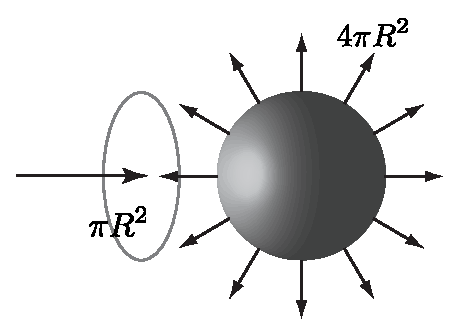
\includegraphics[width=\linewidth]{fig/io.eps}
\end{center}
\caption{Incident starlight onto a planet and thermal emission leaving the planetary surface.}
\label{fig:io}
\end{figure}

The energy received by a planet of radius $R$ can be written using the stellar flux density $S$ as
\begin{align}
\label{eq:lab}
L_{\mathrm{ab}}=(1-A) \pi R^2 S,
\end{align}
where $\pi R^2$ is the planetary cross section (see Fig.~\ref{fig:io}). Here $A$ is the planet-wide reflectivity (albedo), and the factor $(1-A)$ excludes the fraction reflected back to space. If the stellar radiation is approximated as blackbody emission, the stellar flux density is
\begin{align}
\label{eq:starfluxdens}
S= \frac{L_\star}{4 \pi a^2} = \frac{4 \pi R_\star^2 \sigma T_\star^4}{4 \pi a^2}\,\,\mathrm{W/m^2},
\end{align}
where $a$ is the orbital radius, $R_\star$ the stellar radius, $T_\star$ the stellar temperature, and $\sigma$ the Stefan--Boltzmann constant. For Earth, $S_\odot =1370 \,\mathrm{W/m^2}$ is called the solar constant.

If planetary emission is approximated as blackbody radiation at temperature $T_{\mathrm{eq}}$, the emitted power is
\begin{align}
\label{eq:lem}
L_{\mathrm{em}} = \beta \left( 4 \pi R^2 \sigma T_{\mathrm{eq}}^4 \right) + L_\mathrm{int},
\end{align}
where $L_\mathrm{int}$ is the planet's internal heat. For young planets this term can dominate, and such planets are referred to as self-luminous. The parameter $\beta$ characterizes the degree of heat redistribution: $\beta=1$ corresponds to instantaneous, uniform redistribution over the entire globe, while $\beta=0.5$ corresponds to redistribution over only the dayside hemisphere. This factor accounts for close-in, tidally locked planets whose same hemisphere always faces the star, as with the Moon relative to Earth.

For mature planets, internal emission can typically be neglected so that $L_\mathrm{int}=0$. In this case, the absorbed stellar energy should balance the emitted thermal energy,
\begin{align}
\label{eq:lemeqi}
L_{\mathrm{em}} = L_{\mathrm{ab}},
\end{align}
and the temperature $T_{\mathrm{eq}}$ satisfying this condition (radiative equilibrium) is called the \emph{equilibrium temperature}. Combining Eqs.~(\ref{eq:lab})--(\ref{eq:lemeqi}) yields
\begin{align}
\label{eq:eqteq}
\frac{T_{\mathrm{eq}}^4 a^2 }{T_\star^4 R_\star^2} = \frac{1-A}{4 \beta},
\end{align}
or
\begin{align}
&T_\mathrm{eq} = \left(\frac{1-A}{4 \beta}\right)^{\frac{1}{4}} T_\star \sqrt{\frac{R_\star}{a}} \\
&= 396 \,\mathrm{K}\, \left(\frac{1-A}{4 \beta}\right)^{\frac{1}{4}} \left( \frac{T_\star}{5800 \,\mathrm{K}}\right) \left( \frac{R_\star}{R_\odot}\right)^{\frac{1}{2}} \left( \frac{a}{1 \,\mathrm{au}}\right)^{-\frac{1}{2}} \\
&= 396 \,\mathrm{K}\, \left(\frac{1-A}{4 \beta}\right)^{\frac{1}{4}} \left( \frac{L_\star}{L_\odot}\right)^{\frac{1}{4}} \left( \frac{a}{1 \,\mathrm{au}}\right)^{-\frac{1}{2}}.
\end{align}

We also define the mean stellar flux received at the planetary surface. From Eq.~(\ref{eq:lab}),
\begin{align}
\label{eq:aveinpuF}
F_\star &\equiv \frac{L_{\mathrm{ab}}}{4 \pi R^2}= \frac{(1 - A)}{4} S \\
&= 240 \left(\frac{1-A}{0.7}\right) \left(\frac{S}{S_\odot}\right) \mathrm{W/m^2},
\end{align}
which relates directly to $S$. This expression represents the following picture: subtract the reflected fraction from the incident stellar energy, and multiply by the factor $1/4$ that accounts for redistribution by planetary rotation from the illuminated cross section (the disk in Fig.~\ref{fig:io}) over the full spherical surface. The mean absorbed flux density and the equilibrium temperature are related by
\begin{align}
\label{eq:teq}
\sigma T^4_{\mathrm{eq}} = F_\star/\beta.
\end{align}
\subsection*{Radiance and Irradiance}

From a distance, planets and stars appear as point sources, but on closer view they usually exhibit three-dimensional structures with continuous density variations. However, by considering a reference spherical surface --- for example, the planetary surface or the top of the atmosphere for Earth, or the photosphere for a star --- calculations become simpler if we describe radiation \emph{from} or \emph{onto} such a surface. To this end, let us first define quantities that allow us to quantify radiation from, or onto, a finite surface element.

Consider the energy $dE$ passing, per unit time and per unit wavelength, through a solid angle element $d\Omega$ (Fig.~\ref{fig:int}, top) in the direction ${\bf \Omega}$, emitted from an infinitesimal surface element $dA$. Here ${\bf n}$ denotes the unit normal vector. Since $dE$ is proportional to the apparent projected area $\cos{\theta} \, dA$, we can write
\begin{align}
d E = L_{\uparrow}(\theta,\phi) \cos{\theta} \, d A \, d \Omega \, d \nu,
\end{align}
where the proportionality factor $L_{\uparrow}$ is defined as the \emph{radiance}\index{Radiance@Radiance}. This allows us to define radiation independent of projection effects. Its units are, for example, [$\mathrm{W/m^2/sr/\mu m}$].

The net energy flux leaving $dA$ in the direction of ${\bf n}$ is called the \emph{irradiance}\index{Irradiance@Irradiance} $E_{\uparrow}$, given by
\begin{align}
E_{\uparrow} &= \int_{\mathrm{us}} dE = \int  d \Omega \, L_{\uparrow} (\theta,\phi) \cos{\theta} \\
\label{eq:rad}
&= \int_{0}^{2 \pi} d \phi  \int_{0}^{\pi/2} d \theta \, L_{\uparrow} (\theta,\phi) \cos{\theta} \sin{\theta},
\end{align}
where the integration is over the upper hemisphere (us).

\begin{figure}[]
\begin{center}
	\includegraphics[width=\linewidth]{fig/radiance_bw.png}
	\includegraphics[width=\linewidth]{fig/brdfdef_bw.png}
\end{center}
\caption{(Top) Radiation from or onto a surface element $dA$. (Bottom) Incidence of collimated light from direction $(\vartheta_0,\varphi_0)$ and reflection per unit solid angle $d\Omega$ into the same direction.}
\label{fig:int}
\end{figure}

\section{Emission Spectrum}

Let us consider the flux measured at a distance $d$ from a sphere of radius $R_p$ emitting blackbody radiation at temperature $T$. A surface with temperature $T$ emits blackbody radiation, whose radiance is
\begin{align}
L_{\uparrow} d \lambda = B_\lambda (T) d \lambda = \frac{2 h c^2}{\lambda^5} \frac{1}{\exp{(hc/\lambda k_B T)}-1} d \lambda.
\end{align}
Consider the radiation cone $d \Omega$ from a surface element $d A$, and let a telescope with aperture $d A_\mathrm{tel}$ located at distance $d$ be the tip of this cone ($d \Omega = d A_\mathrm{tel}/d^2$). The energy $\Delta E d A_\mathrm{tel}$ received by $d A_\mathrm{tel}$ from $d A$ is then
\begin{eqnarray}
\label{eq:brdfdef3}
\Delta E d A_\mathrm{tel} &=& L_\uparrow \cos{\vartheta_1} d \Omega d A \\
&=& \frac{L_\uparrow}{d^2} \cos{\vartheta_1} d A d A_\mathrm{tel}.
\end{eqnarray}
Thus, the irradiance or flux from the surface element $d A$ as seen by the observer is
\begin{eqnarray}
\label{eq:brdfdef6}
\Delta E = \frac{L_\uparrow}{d^2} \cos{\vartheta_1} d A.
\end{eqnarray}

Integrating over the entire sphere gives
\begin{align}
\label{eq:raddef}
f_p &= \int_\mathrm{planet} \Delta E = \int_\mathrm{planet} d A \frac{B_\nu (T)}{d^2} \cos{\vartheta_1} \\
&= R_p^2 B_\nu (T) \int_0^{2 \pi} d \varphi_1 \int_0^{\pi/2} d \vartheta_1 \sin{\vartheta_1} \cos{\vartheta_1}\\
&= \pi B_\nu (T) \frac{R_p^2}{d^2}.
\end{align}
The total luminosity is obtained by integrating over frequency and multiplying by the surface area of the sphere at distance $d$:
\begin{align}
\label{eq:raddeftot}
L &= 4 \pi d^2 \int_0^{\infty} d \nu \, \pi B_\nu (T) \frac{R_p^2}{d^2} = 4 \pi R_p^2 \sigma T^4.
\end{align}

\begin{itembox}{On the upward flux}
%\tiny
\footnotesize
\color{gray}
In radiative equilibrium models of planetary atmospheres, one typically considers the flux in a one-dimensional vertical column, often imposing the surface flux as a boundary condition. Similarly, let us consider the flux emitted upward from a blackbody surface element. Integrating over the upward hemisphere yields
\begin{align}
\label{eq:defsurf}
F_\nu (T) &= \Delta E = \int_\mathrm{us} d \Omega \, B_\nu (T) \cos{\vartheta_1} = \pi B_\nu (T).
\end{align}
The total flux is obtained by integrating over frequency:
\begin{align}
\label{eq:defsurflum}
F (T) &= \int d \nu \, f_\nu (T) = \sigma T^4.
\end{align}
\end{itembox}

To zeroth order, the emission spectrum of a planet can be approximated by blackbody radiation at a single temperature $T_p$:
\begin{align}
f_p (\lambda) d\, \lambda  &= \pi B_\lambda(\lambda,T_p) \frac{ R_p^2}{d^2}  d \lambda \\
&= \frac{2 \pi h c^2}{\lambda^5} \frac{ R_p^2}{d^2} \left[ \exp{ \left(\frac{h c}{\lambda k_B T_p} \right) }- 1 \right]^{-1} d\, \lambda ,
\label{eq:planckdist}
\end{align}
in some cases.

For example, the Earth's emission spectrum, with little atmospheric absorption, can be roughly approximated by blackbody radiation at surface temperatures $T=200$--$300$ K. However, for gas giants and brown dwarfs, the blackbody approximation is inadequate, primarily due to strong molecular absorption in their atmospheres. The observed spectrum is closer to the blackbody emission from atmospheric layers where the optical depth is near unity, which varies strongly with wavelength due to molecular absorption. These large deviations from blackbody emission are a characteristic signature of exoplanetary atmospheres.

\section{Reflection and Scattering Spectrum}

Reflected light is somewhat more complex because the observed intensity depends on the relative positions of the reflecting surface and the observer. However, on average, it can be treated as follows. In Eq.~(\ref{eq:lab}), the fraction of stellar energy not absorbed by the planet is reflected. Thus, the reflected luminosity is
\begin{align}
    L^\mathrm{ref}_p = A \pi R_p^2 S = \frac{L_\star}{4 \pi a^2} \pi R_p^2 A,
\end{align}
where $A$ is the planetary albedo. The mean reflected flux received at distance $d$ is
\begin{align}
    \langle f_{p}^\mathrm{ref} \rangle = \frac{ L^\mathrm{ref}_p}{4 \pi d^2}.
\end{align}
Using the stellar flux
\begin{align}
    f_\star = \frac{L_\star}{4 \pi d^2},
\end{align}
this can be written as
\begin{align}
    \langle f_{p}^\mathrm{ref} \rangle = \frac{A}{4} \left( \frac{R_p}{a} \right)^2 f_\star.
\end{align}

From a spectral perspective, the key point is that the wavelength dependence arises from the product $A(\lambda) f_\star(\lambda)$, i.e., the stellar spectrum modulated by the planetary reflection spectrum:
\begin{align}
    \langle f_{p}^\mathrm{ref} \rangle (\lambda) d \lambda = \frac{1}{4} \left( \frac{R_p}{a} \right)^2 A(\lambda) f_\star (\lambda) d \lambda.
\end{align}

Computing the flux as a function of orbital phase, rather than as a mean, is somewhat more involved and is omitted here (see Kawahara, \emph{Exoplanet Exploration}, Sec.~5.1.1). Here we simply summarize the result. The reflected flux $f_p^\mathrm{ref} (\lambda)$ observed at distance $d$ is expressed in terms of the star–planet separation $a$, the planetary albedo $A(\lambda)$, the planetary radius $R_p$, the observed stellar flux $f_\star(\lambda)$, and the phase function $\phi(\beta)$, which depends on the star–planet–observer phase angle $\beta$:
\begin{align}
\label{eq:refplanet}
f_p^\mathrm{ref} (\lambda) = \frac{2 \phi(\beta)}{3} A(\lambda) \left(\frac{R_p}{a}\right)^2 f_\star (\lambda),
\end{align}
\begin{align}
\label{eq:phaselambert}
\phi(\beta) \equiv [\sin{\beta} +  (\pi - \beta) \cos{\beta}]/\pi.
\end{align}
Here, $\phi(\beta)$ is the \emph{Lambert phase function}\index{Lambert phase function@Lambert phase function}, a function of the phase angle $\beta = \angle$(star–planet–observer). Note, however, that this relation assumes isotropic scattering. Strongly anisotropic processes, such as specular reflection from oceans (ocean glint), may not follow this approximation.

Although detection of reflected or scattered starlight from exoplanets is currently limited to specific cases such as precise space-based photometry of phase curves, in principle it is a rich source of information about the two-dimensional distribution of planetary surface and atmospheric properties. A key diagnostic in reflected light is the flux ratio between the star and the planet, known as the {\bf star–planet contrast}:
\begin{align}
\label{eq:contrast}
c_{\mathrm{sp}} (\lambda) \equiv \frac{f_p (\lambda)}{f_\star (\lambda)}.
\end{align}
A smaller contrast makes detection easier, both in direct imaging and in phase curve measurements.

For the half-phase geometry ($\beta = 90^\circ$), using Eq.~(\ref{eq:refplanet}), the star–planet contrast can be estimated. For Earth, we obtain
\begin{align}
\label{eq:refplanetearth}
c_\mathrm{sp}  \approx 10^{-10} \left( \frac{A}{0.3} \right) \left(\frac{R_p}{R_\oplus} \right)^{2} \left(\frac{a}{1 \, \mathrm{au}} \right)^{-2},
\end{align}
while for a hot Jupiter,
\begin{align}
\label{eq:refplanethj}
c_\mathrm{sp}  \approx 10^{-6} \left( \frac{A}{0.1} \right) \left(\frac{R_p}{R_J} \right)^{2} \left(\frac{a}{0.05 \, \mathrm{au}} \right)^{-2}.
\end{align}

\section{Various Exoplanet Spectra}

Figure~\ref{fig:earth} shows the spectrum of Earth. In the case of Earth, the atmosphere is relatively thin, so the thermal emission is close to a blackbody spectrum at the radiative equilibrium temperature. The reflection spectrum, on the other hand, corresponds to the stellar spectrum modulated by atmospheric absorption.  

Figure~\ref{fig:bd} shows the spectrum of a brown dwarf. It deviates significantly from a pure blackbody spectrum.  

Figure~\ref{fig:jwst} presents the JWST/NIRSpec spectrum of the hot Saturn WASP-39b, where prominent molecular absorption features are clearly visible.  

\begin{figure}[]
\begin{center}
	\includegraphics[width=\linewidth]{fig/EarthEmis.png}
\end{center}
\caption{Spectrum and contrast of Earth.}
\label{fig:earth}
\end{figure}

\begin{figure}[]
\begin{center}
	\includegraphics[width=\linewidth]{fig/bdspectra.png}
\end{center}
\caption{Spectrum of a brown dwarf, from SpeX Prism library.  Inspired by \cite{2025ApJ...988...31L}.}
\label{fig:bd}
\end{figure}

\begin{figure*}[htb]
\begin{center}
	\includegraphics[width=\linewidth]{fig/jwst_spectrum.png}
\end{center}
\caption{JWST transmission spectrum of WASP-39b \cite{2025ApJ...985..263K}.}
\label{fig:jwst}
\end{figure*}



\chapter{Exoplanet Atmosphere}
\section{Molecular Mixing Ratios in Thermochemical Equilibrium}

In exoplanetary atmospheres, the abundances of molecules are expected to approach thermochemical equilibrium under high-temperature and high-pressure conditions. Even in cases where vertical transport, photochemistry, or low-temperature atmospheres dominate, it is useful to understand the baseline state under thermochemical equilibrium. Here, we consider how the molecular mixing ratios in the atmosphere are determined when thermochemical equilibrium is established. \\

\subsection*{Conservation of Elements}

In the gas, molecular species such as \ce{H2} and \ce{H2O}, as well as atomic species like \ce{H}, ions, and free electrons, are mixed in appropriate proportions. These are collectively referred to as {\bf species}. In contrast, we also wish to track the total number of atoms contained in all species, e.g., \ce{H}, \ce{O}, \ce{C}, etc. These are referred to as {\bf elements}, distinguished from species. In this text, we denote elements using sans-serif fonts, such as $\Hel$, $\Oel$, and $\Cel$. \\


\subsection*{The Case of a Binary System}

As the simplest example, let us consider a two-species gas composed of hydrogen atoms and molecules:
\begin{align*}
\ce{2 H <--> H2}.
\end{align*}
We ask: what composition ratio is reached at thermochemical equilibrium?\footnote{In reality, a third-body catalyst $M$ makes the process more realistic, as in \ce{2 H + M <--> H2 + M}, but here we ignore $M$ for mathematical clarity.}  
In this case, the species are \ce{H} and \ce{H2} ($N_s = 2$), while the only element is $\Hel$ ($N_e = 1$).

Let us suppose there are $\nel_{\Hel}$ atoms of hydrogen (e.g., 1 mol). The element conservation law is then
\begin{align}
    n_\mathrm{H} + 2 n_\mathrm{H2}  = \nel_{\Hel}.
\end{align}
Given pressure $P$ and temperature $T$, the distribution of $\Hel$ between \ce{H} and \ce{H2} at equilibrium is determined by minimizing the Gibbs free energy. At thermochemical equilibrium, the abundances of species are obtained by
\begin{align}
\label{eq:opt1tce}
    &(n_\mathrm{H}^\ast, n_\mathrm{H2}^\ast) = \mathrm{minimize}_{(n_\mathrm{H}, n_\mathrm{H2})} \,\, G(T, P, n_\mathrm{H}, n_\mathrm{H2}) \,\, \\ 
    &\mbox{subject to} \,\, n_\mathrm{H} + 2 n_\mathrm{H2} =  \nel_{\Hel},  \\
    &G(T, P, n_\mathrm{H}, n_\mathrm{H2}) = n_\mathrm{H} \mu_\mathrm{H} + n_\mathrm{H2} \mu_\mathrm{H2}, \\
     &\, n_\mathrm{H} \ge 0, \, n_\mathrm{H2} \ge 0,
\end{align}
where $\mu_\mathrm{H}$ and $\mu_\mathrm{H2}$ are the chemical potentials of \ce{H} and \ce{H2}. Using the standard-state chemical potentials, these are given by
\begin{align}
    \mu_\mathrm{H} &= \mu_\mathrm{H}^o(T) + RT \log{\frac{P_\mathrm{H}}{P_\mathrm{ref}}} \\
    &=  \mu_\mathrm{H}^o(T) + RT \log{\frac{n_\mathrm{H} P}{(n_\mathrm{H} + n_\mathrm{H2}) P_\mathrm{ref}}}, \\
    \mu_\mathrm{H2} &= \mu_\mathrm{H2}^o(T) + RT \log{\frac{P_\mathrm{H2}}{P_\mathrm{ref}}} \\
    &=  \mu_\mathrm{H2}^o(T) + RT\log{\frac{n_\mathrm{H2} P}{(n_\mathrm{H} + n_\mathrm{H2}) P_\mathrm{ref}}}.
\end{align}
One can verify that $\partial G/\partial n_\mathrm{H} = \mu_\mathrm{H}$ and $\partial G/\partial n_\mathrm{H2} = \mu_\mathrm{H2}$ hold.

To prepare for generalization, let us solve the constrained optimization above using the method of Lagrange multipliers. Define the free parameter vector $\xv = ( n_\mathrm{H},  n_\mathrm{H2}, \lambda )^\top$, then
\begin{align}
\label{eq:opt2tce}
    \xv_\ast &= \mathrm{minimize}_{\xv} \,\, \mathcal{L} (T, P, \xv), \\ 
    \mathcal{L} (T, P, \xv) &\equiv G(T, P, \xv) + \lambda (n_\mathrm{H}  + 2 n_\mathrm{H2} - \nel_{\Hel} ), \\
    \label{eq:nonnegative_tce}
    &n_\mathrm{H} \ge 0, \, n_\mathrm{H2} \ge 0.
\end{align}
The non-negativity conditions will be checked afterward. Setting the derivatives of $\mathcal{L} (T, P, \xv)$ with respect to $\xv$ equal to zero gives
\begin{align}
&\frac{\partial \mathcal{L} (T, P, \xv)}{\partial \xv} = 
\begin{pmatrix}
    \mu_\mathrm{H} + \lambda \\
    \mu_\mathrm{H2} + 2 \lambda \\
    n_\mathrm{H} + 2 n_\mathrm{H2} -  \nel_{\Hel} 
\end{pmatrix} \\
&=
\begin{pmatrix}
    \mu_\mathrm{H}^o(T) + RT \log{\frac{n_\mathrm{H} P}{(n_\mathrm{H} + n_\mathrm{H2}) P_\mathrm{ref}}}  + \lambda \\
    \mu_\mathrm{H2}^o(T) + RT\log{\frac{n_\mathrm{H2} P}{(n_\mathrm{H} + n_\mathrm{H2}) P_\mathrm{ref}}} + 2 \lambda \\
    n_\mathrm{H} + 2 n_\mathrm{H2} -  \nel_{\Hel} 
\end{pmatrix}
=
\begin{pmatrix}
    0 \\
    0 \\
    0
\end{pmatrix}.
\end{align}
Eliminating $\lambda$ from the first two components yields
\begin{align}
    \log{\left( \frac{n_\mathrm{H}^2 }{n_\mathrm{H2} (n_\mathrm{H} + n_\mathrm{H2})} \frac{P}{P_\mathrm{ref}} \right)} =- \frac{2 \mu_\mathrm{H}^o - \mu_\mathrm{H2}^o}{RT}.
\end{align}
Using the third component (the conservation law), $n_\mathrm{H} + 2 n_\mathrm{H2} - \nel_{\Hel}=0$, to eliminate $n_\mathrm{H2}$ gives
\begin{align}
\frac{ \nel_{\Hel}^2 - n_\mathrm{H}^2}{4 n_\mathrm{H}^2} = \frac{P}{P_\mathrm{ref}} 
\exp{\left( - \frac{\mu_\mathrm{H2}^o - 2 \mu_\mathrm{H}^o}{RT} \right)}  \equiv k.
\end{align}
Since $n_\mathrm{H} \ge 0$,
\begin{align}
 \frac{n_\mathrm{H}}{ \nel_{\Hel} } = \frac{1}{\sqrt{4 k + 1}}.
\end{align}
From the conservation law,
\begin{align}
 \frac{n_\mathrm{H2}}{ \nel_{\Hel} } = \frac{1}{2} \left( 1 - \frac{1}{\sqrt{4 k + 1}} \right).
\end{align}
Note that these quantities are expressed per hydrogen element $\nel_{\Hel}$. In practice, one can simply set $\nel_{\Hel} = 1$ mol for calculation.

The volume mixing ratios (VMRs) are then
\begin{align}
 \mathrm{VMR} (\ce{H}) &= \frac{n_\mathrm{H}}{n_\mathrm{tot}} = \frac{1}{2} \left( \sqrt{k^2 + 4 k} - k \right), \\
  \mathrm{VMR} (\ce{H2}) &= \frac{n_\mathrm{H2}}{n_\mathrm{tot}} = \frac{1}{2} \left( 2 + k - \sqrt{k^2 + 4 k}\right).
\end{align}
The temperature dependence of the mixing ratios is shown in Fig.~\ref{fig:temperature_exogibbs}. \\

\begin{figure}
    \centering
    \includegraphics[width=\linewidth]{fig/tce_two_species.png}
    \caption{Volume mixing ratios in thermochemical equilibrium for \ce{2 H <--> H2}.}
    \label{fig:temperature_exogibbs}
\end{figure}

\subsection*{Multi-Component Systems$^\ddagger$}

Next, let us consider a multi-element system.  
As an example, take the elements $\Hel, \Cel, \Oel$, and the species \ce{CO, H2, CH4, H2O}. These constitute the major molecular components in hydrogen-rich atmospheres. The relevant chemical reaction can be written as
\begin{align*}
\ce{CO + 3 H2 <--> CH4 + H2O}.
\end{align*}

In terms of elements, the decomposition of each species is
\begin{align*}
\ce{H2 <--> 2 $\Hel$ \, \, \, \, \, \, \, \, \\
H2O <--> 2 $\Hel$ + 1 $\Oel$ \\
CH4 <--> 4 $\Hel$ + 1 $\Cel$ \\
CO <-->  1 $\Cel$ + 1 $\Oel$},
\end{align*}
or, including zero components explicitly,
\begin{align*}
\ce{H2 <--> 2 $\Hel$ + 0 $\Cel$ + 0 $\Oel$ \\
H2O <--> 2 $\Hel$ + 0 $\Cel$ + 1 $\Oel$ \\
CH4 <--> 4 $\Hel$ + 1 $\Cel$ + 0 $\Oel$ \\
CO <--> 0 $\Hel$ + 1 $\Cel$ + 1 $\Oel$ }.
\end{align*}

From the right-hand sides, we define the formula matrix:
\begin{align*}
  A \equiv
\begin{pmatrix} 
2 & 2 & 4 & 0 \\
0 & 0 & 1 & 1 \\
0 & 1 & 0 & 1 
\end{pmatrix}.
\end{align*}

Let the vector of species abundances be $\nv = (n_\mathrm{H_2}, n_\mathrm{H_2 O},n_\mathrm{CH_4},n_\mathrm{CO})^\top$, and the vector of elemental abundances be $\bv = (\nel_\Hel, \nel_\Cel, \nel_\Oel)^\top$ (note the distinction between elemental abundances and species). Then the elemental conservation law is expressed as
\begin{align}
    A \, \nv = \bv.
\end{align}

For a multi-element system, the equilibrium abundances are obtained by minimizing the Gibbs free energy:
\begin{align}
\label{eq:gibss_multi}
    \nv^\ast &= \mathrm{minimize}_{\nv} G(T, p, \nv) \nonumber \\
    &\mbox{subject to} \,\, A \, \nv = \bv, \, n_i \ge 0, \\
    G(T, p, \nv) &\equiv  \muv (T, P, \nv)^\top \nv, \\ 
    \label{eq:chemical_potential_mu}
    \muv (T, p, \nv) &=  \muv^\circ(T) + RT \log{\left(\frac{p}{\ntot} \nv\right)} ,
\end{align}
where the total number density and normalized pressure are defined as
\begin{align}
\label{eq:ntot_tce}
    \ntot &= \sum_i n_i, \\
    p &\equiv P/P_\mathrm{ref}.
\end{align}

For the \ce{CO, H2, CH4, H2O} system, Eq.~(\ref{eq:gibss_multi}) becomes
\begin{align}
    \mathcal{L}(T, p, \nv,\lambdav) &= \sum_{i = \ce{CO, H2, CH4, H2O}} \mu_i (T) \, n_i \nonumber \\ 
    &+ \lambda_{\Hel} (2 n_{\ce{H2}} + 4 n_{\ce{CH4}} + 2 n_{\ce{H2O}} - b_\Hel) \nonumber \\
    &+ \lambda_{\Cel} (n_{\ce{CO}} + n_{\ce{CH4}} - b_\Cel) \nonumber \\ 
    &+ \lambda_{\Oel} (n_{\ce{CO}} + n_{\ce{H2O}} - b_\Oel).
\end{align}

Here we follow the implementation of NASA/CEA (Chemical Equilibrium with Applications) by Gordon and McBride \cite{gordon1994computer,2024arXiv241207166G}. In CEA, minimization of the Gibbs free energy is carried out using a quadratic Lagrange multiplier method. That is,
\begin{align}
    (\nv^\ast, \lambdav)  &= \mathrm{minimize}_{(\nv,\lambdav)} \,\, \mathcal{L}(T, p, \nv, \lambdav), \\
    \mathcal{L}(T, p, \nv,\lambdav) &= G(T, p, \nv) + \lambdav^\top \left(A \nv - \bv\right),
\end{align}
where at this stage the non-negativity condition $n_i \ge 0$ is not yet enforced.

To find stationary points of $\mathcal{L}(T, p, \nv, \lambdav)$, we define, with the optimization variables $\yv = (\nv, \lambdav)$,
\begin{align}
\label{eq:fv_tea0}
    \fv(\yv) &\equiv \frac{\partial}{\partial \yv} \mathcal{L}(T, p, \yv).
\end{align}
The solution is obtained by solving
\begin{align}
    \label{eq:fv_tea}
    \fv(\yv^\ast) = \boldsymbol{0}
\end{align}
using Newton’s method, yielding $\yv^\ast = (\nv^\ast, \lambdav^\ast)$.  

Next, computing the $\nv$-component of Eq.~(\ref{eq:fv_tea0}) gives
\begin{align}
\label{eq:Lpartialn}
    \frac{\partial}{\partial \nv}   \mathcal{L}(T, p, \nv, \lambdav) =  \muv (T, P, \nv) + A^\top \lambdav,
\end{align}
where we have used the thermodynamic identity $\partial_{\nv} G(T, p, \nv) =  \muv (T, P, \nv)$\footnote{This can be verified directly from Eq.~(\ref{eq:chemical_potential_mu}).} together with $\lambdav^\top (A \nv) = (A^\top \lambdav)^\top \nv$ and $\partial_{\xv} (S^\top \xv) = S$.  
Note that Eq.~(\ref{eq:Lpartialn}) is linear in $\lambdav$.  

The $\lambdav$-component simply enforces the conservation relations:
\begin{align}
\label{eq:Lpartiall}
\frac{\partial}{\partial \lambdav}  \mathcal{L}(T, p, \nv, \lambdav) = A \nv - \bv.
\end{align}

Using Eq.~(\ref{eq:chemical_potential_mu}), the system of equations to be solved by Newton’s method in Eq.~(\ref{eq:fv_tea}) is
\begin{align}
\label{eq:Lpartialnx}
    \frac{\muv^\circ(T)}{RT}+ \log{\left(\frac{p}{\ntot^\ast} \nv^\ast \right)} + \frac{A^\top \lambdav^\ast}{RT}   &= \boldsymbol{0}, \\
    A \nv^\ast - \bv &= \boldsymbol{0},
\end{align}
where $\ntot^\ast$ is a function of $\nv^\ast$:
\begin{align}
\ntot^\ast &= \sum_i n_i^\ast.
\end{align}



Here, the CEA algorithm employs several tricks. First, to solve Eq.~(\ref{eq:fv_tea}), we add $\ntot$ as an independent variable. Since $\ntot$ originally depended on $\nv$ via Eq.~(\ref{eq:ntot_tce}), we include this relation—namely Eq.~(\ref{eq:ntot_tce})—as a constraint (rather than as a prerequisite). Furthermore, we reparameterize $\nv$ and $\ntot$ by taking logarithms, i.e., we adopt $\lnnv = \ln{\nv}$ and $\lnntot = \ln{\ntot}$ as independent variables. This transformation naturally enforces the non-negativity constraints $n_i \ge 0$, and, by working in log-space, yields numerically stable computations over a wide dynamic range. 

With these changes, we introduce the new variable set $\zv = (\lnnv, \lambdav, \lnntot)$, and the system to be solved is
\begin{align}
\label{eq:Lpartialncea}
    \Fv_n (\zv) &\equiv \frac{\muv^\circ(T)}{RT} + \lnnv - \lnntot \, \uv + \log{p} \, \uv  + \frac{A^\top \lambdav}{RT},  \\
    \Fv_\lambda (\zv) &\equiv A e^{\lnnv} - \bv = \boldsymbol{0}_M, \\
    F_\mathrm{tot} (\zv) &\equiv \sum_i {e^{q_i}} - e^{\lnntot} = 0,
\end{align}
whose solution satisfies
\begin{align}
  \Fv_n (\zv) &= \boldsymbol{0}_M, \\
  \Fv_\lambda (\zv) &= \boldsymbol{0}_M, \\
  F_\mathrm{tot} (\zv) &= 0.
\end{align}
Here $\boldsymbol{0}_M$ denotes the $M$-dimensional zero vector. The solution is $\zv^\ast = (\lnnv^\ast, \lambdav^\ast, \lnntot^\ast)$. For brevity we sometimes write $\Fv (\zv) = (\Fv_n (\zv), \Fv_\lambda (\zv), F_\mathrm{tot} (\zv))$.

Newton’s method requires the Jacobian $\Jv (\zv) = \partial \Fv / \partial \zv$:
\begin{align}
\label{eq:jacobian_tce}
\Jv (\zv) &=
\left(
\begin{array}{ccc}
    \dfrac{\partial \Fv_n}{\partial \lnnv}  & \dfrac{\partial \Fv_n}{\partial \lambdav}& \dfrac{\partial \Fv_n}{\partial \lnntot}\\ 
    \dfrac{\partial \Fv_\lambda}{\partial \lnnv} & \dfrac{\partial \Fv_\lambda}{\partial \lambdav} & \dfrac{\partial \Fv_\lambda}{\partial \lnntot} \\
    \dfrac{\partial F_\mathrm{tot}}{\partial \lnnv} & \dfrac{\partial F_\mathrm{tot}}{\partial \lambdav} & \dfrac{\partial F_\mathrm{tot}}{\partial \lnntot} \\  
\end{array}
\right) \nonumber \\
&=
\left(
\begin{array}{ccc}
 E_M &  \dfrac{A^\top}{RT} & - \uv\\ 
 Y(\lnnv) & Z_M & \boldsymbol{0}_M \\ 
 (e^{\qv})^\top & \boldsymbol{0}_M^\top & - e^\lnntot\\  
\end{array}
\right),
\end{align}
where $E_M$ is the $M \times M$ identity matrix, $Z_M$ is the $M \times M$ zero matrix, and $M$ is the number of elements (the length of $\bv$). The matrix $Y(\lnnv)$ is defined by
\[
Y(\lnnv)= A \, \mathrm{diag}(e^{\lnnv}),
\]
i.e., with components
\begin{align}
Y_{ij} = A_{ij} e^{q_j}.
\end{align}

From Eq.~(\ref{eq:second_newton}), the Newton update satisfies $\Jv (\zv_k) \, \Delta \zv = - \Fv (\zv_k)$, i.e.,
\begin{align}
    \left(
\begin{array}{ccc}
 E_M &  \dfrac{A^\top}{RT} & - \uv\\ 
 Y(\lnnv) & Z_M & \boldsymbol{0}_M \\ 
 (e^{{\lnnv}_k})^\top & \boldsymbol{0}_M^\top & - e^{(\lnntot)_k}\\  
\end{array}
\right)
    &\left(
\begin{array}{c}
\Delta \lnnv \\
\Delta \lambdav \\
\Delta \lnntot
\end{array}
\right) \nonumber \\
= -
    &\left(
\begin{array}{c}
\Fv_n (\zv_k) \\
\Fv_\lambda(\zv_k) \\
F_\mathrm{tot} (\zv_k)
\end{array}
\right).
\end{align}
Thus the update $\Delta \zv = (\Delta \lnnv, \Delta \lambdav, \Delta \lnntot)$ satisfies
\begin{align}
\label{eq:update_tce_1_}
    &\Delta \lnnv + \frac{A^\top \Delta \lambdav}{RT} - \Delta \lnntot \, \uv \nonumber \\
    &= -\frac{\muv^\circ(T)}{RT} - {\lnnv}_k + (\lnntot)_k \, \uv - \log{p} \, \uv  - \frac{A^\top \lambdav_k}{RT}, \\
\label{eq:update_tce_2_}
    &Y(\lnnv_k) \Delta \lnnv = A \left(e^{\lnnv_k} \odot \Delta \lnnv\right) = \bv - A e^{\lnnv_k}, \\
\label{eq:update_tce_3_}
    &(e^{\lnnv_k})^\top \Delta \lnnv  - e^{(\lnntot)_k} \Delta \lnntot = e^{(\lnntot)_k} - \sum_i {e^{(q_i)_k}} .
\end{align}

Only Eq.~(\ref{eq:update_tce_1_}) involves $\Delta \lambdav$ and $\lambdav_k$. Since we are not directly interested in $\lambdav$, we introduce a new update variable
\begin{align}
    \piv \equiv - \frac{\Delta \lambdav + \lambdav}{RT},
\end{align}
and update $\lnnv, \piv, \lnntot$ instead. (Because $\piv$ is a throwaway variable, we omit $\Delta$ on it.) Then Eq.~(\ref{eq:update_tce_1_}) becomes
\begin{align}
\label{eq:update_tce_1x}
    \Delta \lnnv &=  A^\top \piv + \Delta \lnntot \, \uv - \gv_k(T), \\
    \gv_k (T) &\equiv \frac{\muv^\circ(T)}{RT} + {\lnnv}_k - (\lnntot)_k \, \uv + \log{p} \, \uv .
\end{align}
Hence, once $\piv$ and $\Delta \lnntot$ are determined, we can compute the desired $\Delta \lnnv$. Substituting Eq.~(\ref{eq:update_tce_1x}) into Eqs.~(\ref{eq:update_tce_2_}) and (\ref{eq:update_tce_3_}) yields the following system of $M+1$ linear equations:
\begin{align}
    &A \, \mathrm{diag} (e^{\lnnv_k}) \, A^\top \, \piv + \Delta \lnntot \, A e^{\lnnv_k} \nonumber \\
    &= A \left(e^{\lnnv_k} \odot \gv_k (T) \right) + \bv - A  e^{\lnnv_k}, \\
    &(A  e^{\lnnv_k})^\top \piv + \Delta \lnntot \, \left( \sum_i e^{(\lnnv_k)_i} - e^{(\lnntot)_k} \right) \nonumber \\ 
    &= (e^{\lnnv_k})^\top \gv_k(T) + e^{(\lnntot)_k} - \sum_i {e^{(q_i)_k}} .
\end{align}
In the above, we retained $\lnnv_k$ and $(\lnntot)_k$ explicitly, but in code it is often clearer to revert $e^{\lnnv}$ to $\nv$. Define
\begin{align}
    B &\equiv  A \, \mathrm{diag} (\nv_k) \, A^\top, \\
    \bv_k &\equiv A \nv_k, \\
    \delta \bv_k &\equiv \bv - \bv_k, \\
     \delta n_\mathrm{tot,k} &\equiv  \sum_i n_{k,i} - (n_\mathrm{tot})_{k},
\end{align}
where $n_{k,i}$ denotes the $i$-th component of $\nv_k$. Then we obtain
\begin{align}
\label{eq:rgie1}
   B \, \piv + \Delta \lnntot \, \bv_k &= A \left( \nv_k \odot \gv_k (T) \right) + \delta \bv_k, \\
\label{eq:rgie2}
\bv_k \cdot \piv + \delta n_\mathrm{tot, k} \, \Delta \lnntot &= \nv_k \cdot \gv_k(T) - \delta n_\mathrm{tot,k}.
\end{align}
This linear system in $\piv$ and $\Delta \lnntot$ is referred to as the \emph{Reduced Gibbs Iteration Equations}.

\section{Vibrational–Rotational Transitions of Diatomic Molecules}

\begin{figure}[]
 \begin{center}
	\includegraphics[width=1.0\linewidth]{fig/co_ele_state.png}
% \includegraphics[bb=0 0 474 461,width=1.0\linewidth]{fig/orbele.png}
\end{center}
\caption{Electronic states of carbon monoxide. The horizontal axis is the internuclear distance (carbon–oxygen).}
\label{fig:co_ele_state}
\end{figure} 

In diatomic molecules, quantum-mechanical transitions arise from combinations of electronic, vibrational (nuclear), and rotational (nuclear) level transitions. For the electronic levels, because nuclear motion is much slower than electronic motion, one can solve the electronic wave equation with the internuclear distance $r$ fixed and obtain the corresponding electronic eigenenergies.

As $r$ is slowly varied, the ground-state electronic eigenenergy changes continuously with $r$. Figure~\ref{fig:co_ele_state} shows (a subset of) the electronic eigenenergies of carbon monoxide as a function of the internuclear distance $r$. In the context of molecular absorption in exoplanet atmospheres, it is generally safe to assume that the electronic state is the ground state ( in the case of CO, $\mathrm{X^1}\Sigma^+$)\footnote{Electronic transitions are occasionally considered as well.}. Thus, the ground-state electronic eigenenergy can be written as a function of $r$ as $V(r)$, and the two nuclei can be regarded as moving in the potential $V(r)$.

\begin{itembox}{{\it column} -- Labels of Electronic States $\,^\dagger$}
%\tiny
\footnotesize
For diatomic molecules, the magnitude $\Lambda$ of the projection of the total electronic orbital angular momentum onto the molecular axis ($Z$ axis), $L_z$, is conserved, and $\Lambda$ serves as a label for the electronic state. The spectroscopic symbols corresponding to each $\Lambda$ are summarized in Table~\ref{tab:spesymbol}. As in atoms, spin multiplicity exists for molecules. With total spin $S$ ($S=0,1/2,1,3/2,\cdots$), the multiplicity is $2S+1$, written to the upper left of $\Lambda$:
\begin{eqnarray}
    \,^{2S+1} \Lambda.
\end{eqnarray}
If the diatomic molecule consists of two identical atoms (homonuclear diatomic), the wavefunction under exchange of the two nuclei transforms as $\Psi \to \pm \Psi$. The symbol \emph{u} (ungerade) is appended as a subscript when the sign changes, and \emph{g} (gerade) when it does not. In addition, for $\Sigma$ states, the sign change under reflection through a plane containing the molecular axis is indicated by a superscript $\pm$. Altogether, an electronic state can be labeled, for example, as
\begin{eqnarray}
    \,^{2} \Sigma_u^+ .
\end{eqnarray}
Table~\ref{tab:elebase} lists the ground states of representative diatomic molecules. Among electronic states with the same spin multiplicity, one may also prepend capital letters X, B, C, D, $\cdots$ (including the ground state) in increasing energy order. For states with spin multiplicity different from that of the ground state, lowercase letters b, c, d, $\cdots$ are sometimes used in increasing energy order; e.g.,
$X\,^1 \Sigma_g^+$ (ground state), $B\,^1 \Sigma_u^+$, $C\,^1 \Sigma_u^+$, …, $a\,^3 \Sigma$, …
\end{itembox}

\begin{table}[]
    \centering
    \begin{tabular}{c|cccccc}
    \hline\hline
        $L$ & 0 & 1 & 2 & 3 & $\cdots$  \\
        \hline
          & S & P & D & F & $\cdots$  \\
          Degeneracy & 1 & 3 & 5 & 7 & (2$L$+1) \\
        \hline\hline
        $\Lambda$ & 0 & 1 & 2 & 3 & $\cdots$  \\
        \hline
        & $\Sigma$ & $\Pi$ & $\Delta$ & $\Phi$ & $\cdots$ \\
        Degeneracy & 1 & 2 & 2 & 2 &  
    \end{tabular}
    \caption{Correspondence between the electronic orbital angular momentum $L$ for atoms and the absolute value of the molecular-axis projection $L_z$ for diatomic molecules, $\Lambda$, and the spectroscopic symbols. For atoms the degeneracy is $2L+1$, whereas for molecules (except for $\Lambda=0$), the two projections $L_z=\pm \Lambda$ lead to twofold degeneracy.}
    \label{tab:spesymbol}
\end{table}

\begin{table}[]
    \centering
    \begin{tabular}{c|c}
    \hline\hline
    Molecule & Ground State\\
    \hline
        \ce{H2} & $\,^1 \Sigma_g^+$\\
        \ce{N2} & $\,^1 \Sigma_g^+$\\
        \ce{O2} & $\,^3 \Sigma_g^-$\\
        \ce{CO} &  $\,^1 \Sigma$\\
        \ce{CN} &  $\,^2 \Sigma$\\
        \ce{NO} &  $\,^2 \Pi$
    \end{tabular}
    \caption{Electronic ground states of representative diatomic molecules.}
    \label{tab:elebase}
\end{table}

Let us now consider the energy levels of a freely moving diatomic molecule, such as carbon monoxide (CO) in an atmosphere, which consists of two nuclei with different masses $m_1$ and $m_2$ and multiple electrons. Assuming the electrons remain in the ground state, the system can be treated as two nuclei moving in the potential $V(r)$, where $r$ is the internuclear distance. As illustrated in the ground state of Fig.~\ref{fig:co_ele_state}, $V(r)$ attains its minimum value (we define it by $V_e$) at $r=r_e \sim 1.2 \AA$, and the two nuclei undergo rotational motion and vibrational motion about the equilibrium distance $r_e$.

\begin{figure}[h]
\begin{center}
%  \includegraphics[width=70mm]{fig_left.PNG}
  \includegraphics[width=\linewidth]{fig/fig_right.PNG}
\end{center}
\vspace*{-5mm}
\caption{Coordinates of the nuclei in a diatomic molecule.}
\label{fig:phys2_fig1}
\end{figure}

Assuming that $V(r)$ is known, we focus on the nuclear wave equation.  
With nuclear coordinates taken as in Fig.~\ref{fig:phys2_fig1}, the nuclear wave equation can be written as
\begin{align}
\label{eq:phys2_shro}
&\left( - \frac{\hbar^2}{2 m_1} \nabla_{1}^2  - \frac{\hbar^2}{2 m_2} \nabla_{2}^2 + V(r) \right) \psi(\boldsymbol{r}_1, \boldsymbol{r}_2) \nonumber \\
&= E \psi(\boldsymbol{r}_1, \boldsymbol{r}_2),
\end{align}
where $\boldsymbol{r}_1$ and $\boldsymbol{r}_2$ are the position vectors of nuclei 1 and 2, respectively, and their separation is $r = |\boldsymbol{r}_1 - \boldsymbol{r}_2|$. The operators $\nabla_{1}^2$ and $\nabla_{2}^2$ are the Laplacians for nuclei 1 and 2; $\hbar = h/(2\pi)$ with $h$ the Planck constant; $E$ is the eigenvalue of the nuclear wave equation; and $\psi(\boldsymbol{r}_1, \boldsymbol{r}_2)$ is the nuclear wavefunction. By solving Eq.~(\ref{eq:phys2_shro}), we consider vibrational–rotational transitions of the nuclei.

Define the center-of-mass coordinate
\[
\boldsymbol{R} = \frac{m_1 \boldsymbol{r}_1 + m_2 \boldsymbol{r}_2}{m_1 + m_2},
\]
and the relative coordinate $\boldsymbol{r} = \boldsymbol{r}_1 - \boldsymbol{r}_2$.  
With the reduced mass $\mu = (m_1^{-1} + m_2^{-1})^{-1}$ and the total mass $M = m_1 + m_2$, the wave equation in center-of-mass and relative coordinates becomes
\begin{align}
\label{eq:com_each}
\left( - \frac{\hbar^2}{2 \mu} \nabla_{r}^2  - \frac{\hbar^2}{2 M} \nabla_{R}^2 + V(r) \right) \psi(\boldsymbol{r},\boldsymbol{R}) = E \psi(\boldsymbol{r},\boldsymbol{R}).
\end{align}
Here we have defined the Laplacians
\[
\nabla^2_{R} = \frac{\partial^2}{\partial X^2} +  \frac{\partial^2}{\partial Y^2} +  \frac{\partial^2}{\partial Z^2}, \qquad
\nabla^2_{r} = \frac{\partial^2}{\partial x^2} +  \frac{\partial^2}{\partial y^2} +  \frac{\partial^2}{\partial z^2}.
\]

\begin{itembox}{$\clubsuit$ Eq.~(\ref{eq:com_each}) $\,^\dagger$}
%\tiny
\footnotesize
Let $(X,x)$, $(Y,y)$, and $(Z,z)$ denote the first, second, and third Cartesian components of $\boldsymbol{R}$ and $\boldsymbol{r}$, respectively.  
From the transformations
\begin{align}
x &= x_1 - x_2, \qquad
X = \frac{m_1 x_1 + m_2 x_2}{M}, \nonumber
\end{align}
we have
\begin{eqnarray}
\frac{\partial}{\partial x_1} &=& \frac{\partial x}{\partial x_1} \frac{\partial}{\partial x} +
\frac{\partial X}{\partial x_1} \frac{\partial}{\partial X}
=  \frac{\partial}{\partial x} +  \frac{m_1}{M}\frac{\partial}{\partial X},
\end{eqnarray}
which leads to
\begin{align}
\label{eq:x1}
\frac{1}{m_1}\frac{\partial^2}{\partial x_1^2} =
\frac{1}{m_1} \frac{\partial^2}{\partial x^2} + \frac{m_1}{M^2} \frac{\partial^2}{\partial X^2}
+ \frac{2}{M}\frac{\partial}{\partial x}\frac{\partial}{\partial X}.
\end{align}
Similarly,
\begin{eqnarray}
\frac{\partial}{\partial x_2} &=& \frac{\partial x}{\partial x_2} \frac{\partial}{\partial x} +
\frac{\partial X}{\partial x_2} \frac{\partial}{\partial X}
=  - \frac{\partial}{\partial x} +  \frac{m_2}{M}\frac{\partial}{\partial X},
\end{eqnarray}
so that
\begin{align}
\label{eq:x2}
\frac{1}{m_2}\frac{\partial^2}{\partial x_2^2} =
\frac{1}{m_2} \frac{\partial^2}{\partial x^2} + \frac{m_2}{M^2} \frac{\partial^2}{\partial X^2}
- \frac{2}{M}\frac{\partial}{\partial x}\frac{\partial}{\partial X}.
\end{align}
From (\ref{eq:x1}) and (\ref{eq:x2}),
\begin{align}
\frac{1}{m_1} \frac{\partial^2}{\partial x_1^2} +  \frac{1}{m_2} \frac{\partial^2}{\partial x_2^2} =
\frac{1}{\mu}\frac{\partial^2}{\partial x^2} + \frac{1}{M}\frac{\partial^2}{\partial X^2}.
\end{align}
Likewise,
\begin{align}
\frac{1}{m_1} \frac{\partial^2}{\partial y_1^2} +  \frac{1}{m_2} \frac{\partial^2}{\partial y_2^2} &=
\frac{1}{\mu}\frac{\partial^2}{\partial y^2} + \frac{1}{M}\frac{\partial^2}{\partial Y^2}, \\
\frac{1}{m_1} \frac{\partial^2}{\partial z_1^2} +  \frac{1}{m_2} \frac{\partial^2}{\partial z_2^2} &=
\frac{1}{\mu}\frac{\partial^2}{\partial z^2} + \frac{1}{M}\frac{\partial^2}{\partial Z^2}.
\end{align}
Adding these and multiplying by $- \hbar^2/2$ gives
\begin{align}
- \frac{\hbar^2}{2 m_1} \nabla_{1}^2  - \frac{\hbar^2}{2 m_2} \nabla_{2}^2 
= - \frac{\hbar^2}{2 \mu} \nabla_{r}^2  - \frac{\hbar^2}{2 M} \nabla_{R}^2 .
\end{align}
\end{itembox}

For Eq.~(\ref{eq:com_each}), separate variables by writing $\psi(\boldsymbol{R},\boldsymbol{r}) = \Phi(\boldsymbol{R}) \phi(\boldsymbol{r})$ and $E = E_R + E_r$, where $E_R$ and $E_r$ are the eigenenergies of the center-of-mass and relative motions, respectively. Then
\begin{align}
&\Phi(\boldsymbol{R}) \left( - \frac{\hbar^2}{2 \mu} \nabla_{\boldsymbol{r}}^2 \phi(\boldsymbol{r})  + V(r) \phi(\boldsymbol{r}) - E_r \phi(\boldsymbol{r})  \right) \nonumber \\
&+ \phi(\boldsymbol{r}) \left(  - \frac{\hbar^2}{2 M} \nabla_{\boldsymbol{R}}^2 \Phi(\boldsymbol{R}) - E_R \Phi(\boldsymbol{R}) \right) = 0,
\end{align}
which yields the center-of-mass and relative-motion equations:
\begin{align}
- \frac{\hbar^2}{2 M} \nabla_{\boldsymbol{R}}^2 \Phi(\boldsymbol{R}) &= E_R \Phi(\boldsymbol{R}), \\
- \frac{\hbar^2}{2 \mu} \nabla_{\boldsymbol{r}}^2 \phi(\boldsymbol{r})  + V(r) \phi(\boldsymbol{r}) &= E_r \phi(\boldsymbol{r}).
\end{align}
The center-of-mass equation describes the translational motion of the molecule as a whole (e.g., plane-wave solutions).

Next, for the relative-motion equation, introduce spherical coordinates $(r,\varphi,\theta)$ and separate variables as
\begin{eqnarray}
\label{eq:rotvib}
\phi(\boldsymbol{r}) = \frac{\phi_r(r)}{r} Y(\varphi, \theta).
\end{eqnarray}
The radial equation for $\phi_r(r)$ reduces to a one-dimensional wave equation in the effective potential $V_\mathrm{eff}(r) = V(r) + W(r)$, where $W(r)$ is the centrifugal term arising from rotation. We now determine $W(r)$.

The Laplacian in spherical coordinates is
\begin{align}
\nabla^2_{r, \varphi, \theta} &= \frac{1}{r^2} \left( \frac{\partial}{\partial r} r^2 \frac{\partial}{\partial r} + \nabla^2_{\varphi, \theta} \right), \\
\nabla^2_{\varphi, \theta} &= \frac{1}{\sin{\theta}}\frac{\partial}{\partial \theta}
\left( \sin{\theta} \frac{\partial}{\partial \theta} \right)
+ \frac{1}{\sin^2 \theta} \frac{\partial^2}{\partial \varphi^2},
\end{align}
and the spherical harmonics $Y_{lm}(\varphi,\theta)$ satisfy
\begin{eqnarray}
\nabla^2_{\varphi, \theta} Y_{lm}(\varphi, \theta) + J(J+1) Y_{lm}(\varphi, \theta) = 0,
\end{eqnarray}
where $J=0,1,2,\dots$ is the rotational quantum number and $m$ is an integer with $|m| \le J$.

Substituting Eq.~(\ref{eq:rotvib}) into the relative-motion equation and expressing the Laplacian in spherical coordinates, we obtain
\begin{align}
&- \frac{\hbar^2}{2 \mu} \left( \frac{1}{r^2} \frac{\partial }{\partial r} r^2 \frac{\partial }{\partial r} + \frac{1}{r^2} \nabla^2_{\varphi,\theta} \right) \frac{\phi_r(r)}{r} Y(\varphi, \theta) \nonumber \\
&+ V(r) \frac{\phi_r(r)}{r} Y(\varphi, \theta) = E_r \frac{\phi_r(r)}{r} Y(\varphi, \theta),
\end{align}
which separates to
\begin{align}
\label{eq:separation_vari}
&\frac{r^2}{ \phi_r(r)}\frac{\partial^2}{\partial r^2} \phi_r(r) + \frac{2 \mu r^2}{\hbar^2} (E_r - V(r)) \nonumber \\
&= - \frac{\nabla^2_{\varphi,\theta} Y(\varphi,\theta)}{Y(\varphi,\theta)}.
\end{align}
Setting the right-hand side to $J(J+1)$ identifies $Y(\varphi,\theta)$ with the spherical harmonics $Y_{lm}(\varphi,\theta)$.


\begin{itembox}{$\clubsuit$ Equation (\ref{eq:separation_vari}) $\,^\dagger$}
%\tiny
\footnotesize
\begin{align}
  &\frac{\partial}{\partial r} \left(r^2 \frac{\partial}{\partial r} \frac{\phi_r}{r} \right)
  = \frac{\partial}{\partial r} \left( r^2 \frac{r \phi_r^\prime - \phi_r}{r^2}\right) \nonumber \\
  &= \frac{\partial}{\partial r} ( r \phi_r^\prime - \phi_r)
  = \phi_r^\prime + r \phi_r^{\prime\prime} - \phi_r^\prime \nonumber \\ 
  &= r \frac{\partial^2}{\partial r^2} \phi_r(r)
\end{align}
\end{itembox}

Then the radial wave equation becomes
\begin{align}
&- \frac{\hbar^2}{2 \mu} \frac{\partial^2}{\partial r^2} \phi_r(r)
+ \left(  V(r) + \frac{\hbar^2 J(J+1)}{2 \mu r^2} \right) \phi_r(r) \nonumber \\
&= E_r \phi_r(r),
\end{align}
which can be regarded as one-dimensional motion in the effective potential
\begin{align}
V_\mathrm{eff} (r) = V(r) + \frac{\hbar^2 J(J+1)}{2 \mu r^2}.
\end{align}
Hence,
\begin{align}
W(r) = \frac{\hbar^2 J(J+1)}{2 \mu r^2}.
\end{align}

\begin{figure*}
    \centering
    \includegraphics[width=\linewidth]{fig/branch_13_0.png}
    \caption{R-branch and P-branch cross sections in the $\Delta \nu=1$ band of carbon monoxide.}
    \label{fig:rpbranchco}
\end{figure*}

For the eigenvalue $E_r$ of the relative motion, we denote quantum states by the pair $(\nu, J)$ of vibrational quantum number $\nu$ and rotational quantum number $J$, with the initial state $(\nu,J) = (\nu_i, J_i)$ and the final state $(\nu,J) = (\nu_f, J_f)$. Consider transitions in a diatomic molecule such as carbon monoxide with $\Delta \nu = \nu_f - \nu_i = 1$ and $\Delta J = J_f - J_i = \pm 1$. Denote the eigenvalues of the relative motion for the initial and final states by $E_r = E_{r,i}$ and $E_r = E_{r,f}$, respectively, and define the transition energy $\Delta E = E_{r,f} - E_{r,i}$.

Make the coordinate transformation $q=r - r_e$. Then
\begin{align}
\label{eq:vpotent}
V_\mathrm{eff} (q) &\approx V_e + \frac{\mu}{2} \omega^2 q^2 + \frac{\hbar^2 J(J+1)}{2 \mu (q + r_e)^2} \\
&\approx V_e + \frac{\mu}{2} \omega^2 q^2 + \frac{\hbar^2 J(J+1)}{2 \mu  r_e^2},
\end{align}
so the wave equation for $\phi_r(q)$ is
\begin{align}
&- \frac{\hbar^2}{2 \mu} \frac{\partial^2}{\partial q^2} \phi_r(q) + \frac{\mu}{2} \omega^2 q^2 \phi_r(q) = E^\prime_r \phi_r(q) \\
&E^\prime = E_r - V_e - \frac{\hbar^2 J(J+1)}{2 \mu r_e^2},
\end{align}
i.e., the harmonic-oscillator wave equation. The energy eigenvalues of a harmonic oscillator with angular frequency $\omega$, with vibrational quantum number $\nu=0,1,2,\dots$, are
\begin{align}
E^\prime = \hbar \omega \left( \nu + \frac{1}{2} \right),
\end{align}
so the eigenvalues of the original wave equation are
\begin{align}
E_r = V_e + \hbar \omega \left( \nu + \frac{1}{2} \right) + \frac{\hbar^2 J(J+1)}{2 \mu r_e^2}.
\end{align}

Let
\begin{align}
E_r(\nu,J) = V_e + \hbar \omega \left( \nu + \frac{1}{2} \right) + \frac{\hbar^2 J(J+1)}{2 \mu r_e^2}.
\end{align}
Since $E_{r,f} = E(\nu_f, J_f)$ and $E_{r,i}=E(\nu_i,J_i)$, we have
\begin{align}
\Delta E &= E_{r,f} - E_{r,i} = E(\nu_f, J_f) - E(\nu_i,J_i) \\
&= \hbar (\nu_f - \nu_i) + \frac{\hbar^2}{2 \mu r_e^2} \bigl[J_f(J_f+1) - J_i(J_i+1)\bigr] \\
&= \hbar \Delta \nu + \frac{\hbar^2}{2 \mu r_e^2} (J_f-J_i)(J_f + J_i + 1) \\
\label{eq:nl}
&= \hbar \Delta \nu + \frac{\hbar^2}{2 \mu r_e^2} \Delta J \,(2 J_i + \Delta J + 1).
\end{align}

Substituting $\Delta \nu = 1$, $\Delta J = 1$ into Eq.~(\ref{eq:nl}) yields
\begin{align}
\label{eq:rbranch}
\Delta E = \hbar \omega + \frac{\hbar^2}{\mu r_e^2} (1 + J_i).
\end{align}
Substituting $\Delta \nu = 1$, $\Delta J = -1$ into Eq.~(\ref{eq:nl}) gives
\begin{align}
\label{eq:pbranch}
\Delta E = \hbar \omega - \frac{\hbar^2}{\mu r_e^2} J_i.
\end{align}

These results imply that, centered on $\hbar \omega$, the transitions form a comb with spacing $\frac{\hbar^2}{\mu r_e^2}$ to either side. Figure~\ref{fig:rpbranchco} shows the cross sections of CO for $\Delta \nu =1$, displaying this comb-like pattern. The series of lines given by Eq.~(\ref{eq:rbranch}), extending toward higher wavenumber (to the right), is the \emph{R-branch}, and that of Eq.~(\ref{eq:pbranch}) is the \emph{P-branch}.

\section{Line Profiles and Line Strengths}

Although the transition energies of molecules are discrete due to quantum-mechanical effects, the absorbed energy is broadened around those discrete energies for various reasons. This broadening is called \emph{broadening}. In planetary atmospheres, the three important types are
\begin{itemize}
    \item Doppler broadening due to thermal motion (and microturbulence),
    \item natural broadening due to the uncertainty principle,
    \item pressure broadening that depends on pressure and arises from van der Waals forces between molecules.
\end{itemize}

First, broadening due to thermal motion is caused by the Doppler shift $\nu = \hat{\nu} ( 1 + v_x/c)$ when an atom has a line-of-sight velocity $v_x$ owing to thermal motion. Because the distribution function of $v_x$ follows the Maxwell velocity distribution,
\begin{align}
P(v_x) &= \sqrt{\frac{m}{2 \pi k_B T}} \, e^{-\frac{m v_x^2}{2 k_B T}} \\
&= \sqrt{\frac{m}{2 \pi k_B T}} \, e^{-\frac{m c^2 (\nu - \hat{\nu})^2}{2 k_B T \hat{\nu}^2}},
\label{eq:dopplerveldist}
\end{align}
the line is broadened accordingly. Using the half width at half maximum (HWHM),
\begin{eqnarray}
\gamma_D = \hat{\nu} \sqrt{\frac{2 (\log{2}) k_B T}{m c^2}},
\label{eq:dopplergamma}
\end{eqnarray}
the Doppler-broadened line profile is
\begin{align}
g_D(\nu; \hat{\nu}; \gamma_D) = \sqrt{\frac{\log{2}}{\pi}} \frac{1}{\gamma_D}
\exp\!\left[ - \log{2} \left( \frac{\nu - \hat{\nu}}{\gamma_D}\right)^2 \right],
\label{eq:dopplerprofile}
\end{align}
i.e., Doppler broadening follows a Gaussian distribution. Velocity dispersion from microturbulence is likewise often approximated by a Gaussian, but is not commonly considered at present.

By contrast, pressure broadening and natural broadening are both represented by the Lorentz profile,
\begin{eqnarray}
g_L(\nu; \hat{\nu}; \gamma_L) = \frac{\gamma_L/\pi}{(\nu - \hat{\nu})^2  + \gamma_L^2},
\label{eq:lorentzprofile}
\end{eqnarray}
where $\gamma_L$ is the HWHM.

In planetary atmospheres, pressure broadening (van der Waals broadening) is especially important. For Earth’s atmosphere, one often uses the air-broadening coefficient $\gamma_{L, \mathrm{W}}^{\mathrm{air}}$, defined as $\gamma_{L, \mathrm{W}}$ at $p_0=$ 1 atmosphere and $T_0=$ 296 K, and computes
\begin{eqnarray}
\gamma_{L, \mathrm{W}}(p,T) = \gamma_{L, \mathrm{W}}^{\mathrm{air}} \frac{p}{p_0} \left( \frac{T_0}{T} \right)^\alpha,
\label{eq:airtogen}
\end{eqnarray}
where $\alpha$ is the temperature exponent (typically around 0.5, but it varies). Because pressure broadening originates from van der Waals forces exerted by surrounding molecules, it depends on the background gas composition. In particular, many exoplanet atmospheres are H$_2$/He-dominated, so values differ from those under Earth air, and care is needed.

Natural broadening is the line broadening arising from the uncertainty principle. Using the Einstein $A$ coefficient,
\begin{eqnarray}
\gamma_{L, \mathrm{n}} = \frac{A}{4 \pi c} = \frac{0.222}{4 \pi c} \left( \frac{\nu}{\mathrm{cm^{-1}}} \right)^2 \mathrm{[cm^{-1}]},
\end{eqnarray}
which reflects the excited-state survival probability $\propto e^{-A t}$ and the uncertainty relation. Unlike pressure broadening, natural broadening is more significant at low pressure.

When both the Doppler and Lorentz profiles apply, the line profile is their convolution, called the \emph{Voigt profile}\index{Voigt profile@Voigt profile}:
\begin{align}
&g_V(\nu;\hat{\nu}) = ( g_L \ast g_D )(\nu; \hat{\nu}) \nonumber \\
&= \int_{-\infty}^\infty \! d \nu^\prime \,
g_L(\nu - \nu^\prime;\hat{\nu};\gamma_L)\,
g_D(\nu^\prime - \hat{\nu};\hat{\nu};\gamma_D).
\label{eq:voigt}
\end{align}
If both pressure and natural broadening contribute, one may use
\begin{eqnarray}
\label{eq:sumgamma}
\gamma_L = \gamma_{L, \mathrm{W}} + \gamma_{L, \mathrm{n}},
\end{eqnarray}
because the convolution of two Lorentzians satisfies
\begin{align}
&g_L(\nu;\hat{\nu},\gamma_{L,\mathrm{W}}) \ast g_L(\nu;\hat{\nu},\gamma_{L,\mathrm{n}}) \nonumber \\
&= \int_\infty^\infty \! d \nu^\prime \,
g_L(\nu - \nu^\prime;\hat{\nu};\gamma_{L,\mathrm{W}})\,
g_L(\nu^\prime - \hat{\nu};\hat{\nu};\gamma_{L,\mathrm{n}}) \\
&= \frac{(\gamma_{L,\mathrm{W}}+\gamma_{L,\mathrm{n}})/\pi}{(\nu - \hat{\nu})^2  + (\gamma_{L,\mathrm{W}}+\gamma_{L,\mathrm{n}})^2} \nonumber \\
&= g_L(\nu;\hat{\nu},\gamma_{L,\mathrm{W}}+\gamma_{L,\mathrm{n}}),
\label{eq:voigt2}
\end{align}
so the HWHMs add. Note also that Lorentzian wings are not thought to extend indefinitely; beyond a certain distance from line center (on the order of $10^2\,\mathrm{cm^{-1}}$), a rapid cutoff (sub-Lorentzian behavior) is expected. Although this effect is not yet fully understood, one should take care when computing over wide wavenumber ranges.

Because line profiles are normalized as
\begin{align}
\int d \nu \, g(\nu) = 1,
\end{align}
the dimension of $g(\nu)$ is $\mathrm{cm}$.

Consider the absorption of photons by molecules. In molecular spectroscopy, it is common to express energies as wavenumbers by dividing by $hc$; we follow that convention. Since we consider absorption, the final state lies at higher energy than the initial state; we therefore relabel the final and initial states as \textit{upper} and \textit{lower}, respectively. For example, $E_\mathrm{low} = E_{\nu_i, J_i}/hc$ and $E_\mathrm{up} = E_{\nu_f, J_f}/hc$.

The strength of each absorption line is proportional to the number of molecules in the lower state $E_\mathrm{low}$, because absorption proceeds via stimulated absorption from that level. However, stimulated emission induced by the incident light reduces the effective absorption and must be included. Under local thermodynamic equilibrium,
\begin{align}
\label{eq:lte}
\frac{n_\mathrm{low}}{n} &= \frac{\mathsf{g}_\mathrm{low}}{Q(T)}
\exp\!\left(- \frac{h c E_\mathrm{low}}{k_B T} \right),
\end{align}
where $\mathsf{g}_\mathrm{low}$ is the degeneracy, $n$ is the total population, and $Q(T)$ is the partition function. The correction for stimulated emission is $(1- e^{-h c \hat{\nu}/k_B T})$, where $\hat{\nu}$ is the absorption wavenumber, i.e., the level spacing $\hat{\nu} = E_\mathrm{up} - E_\mathrm{low}$\footnote{We avoid writing this quantity directly with $E$ because, spectroscopically, the relevant observable is the wavenumber at the absorption center.}.

Including the coefficients, the \emph{line strength} is defined so that the cross section is
\begin{align}
\sigma^2 (\nu) = S(T)\, g(\nu),
\end{align}
i.e., $S(T)$ has the dimension of $\mathrm{cm}$. One obtains
\begin{align}
\label{eq:STexomol}
S(T) &= \frac{\mathsf{g}_\mathrm{up}}{Q(T)} \frac{ A}{8 \pi c \hat{\nu}^2}
e^{-  c_2 E_\mathrm{low}/T} \left(1- e^{-c_2 \tilde{\nu}/T}\right),
\end{align}
where $c_2 \equiv hc/k_B = 1.4387773 \, \mathrm{cm\,K}$ and $A$ is the Einstein $A$ coefficient.

\begin{itembox}{$\clubsuit$ Eq.~(\ref{eq:STexomol}) $\,^\dagger$}
%\tiny
\footnotesize
The effective absorption equals stimulated absorption ($B_{lu}$) minus stimulated emission ($B_{ul}$):
\begin{align}
S(T) &= \frac{h c \hat{\nu}}{c} \left( \frac{n_\mathrm{low}}{n} B_{lu} - \frac{n_\mathrm{up}}{n} B_{ul} \right).
\end{align}
Under LTE,
\begin{align}
\frac{n_\mathrm{up}}{n_\mathrm{low}} &= \frac{\mathsf{g}_\mathrm{up}}{\mathsf{g}_\mathrm{low}}
\exp\!\left(- \frac{h c (E_\mathrm{up} - E_\mathrm{low})}{k_B T} \right) \\
&= \frac{\mathsf{g}_\mathrm{up}}{\mathsf{g}_\mathrm{low}} e^{-hc \hat{\nu}/k_B T}.
\end{align}
From detailed balance,
\begin{align}
\mathsf{g}_\mathrm{low} B_{lu} &= \mathsf{g}_\mathrm{up} B_{ul}, \\
A &= 2 \pi h c \hat{\nu}^3 B_{ul}.
\end{align}
Using these,
\begin{align}
S(T) &= \frac{h \hat{\nu}}{4 \pi} \frac{n_\mathrm{low}}{n} B_{lu} \left(1 -  e^{-hc \hat{\nu}/k_B T}\right) \\
&= \frac{\mathsf{g}_\mathrm{up}}{Q(T)} \frac{ A}{8 \pi c \hat{\nu}^2}
e^{- h c E_\mathrm{low}/k_B T} \left(1- e^{- h c \tilde{\nu}/k_B T}\right),
\end{align}
where Eq.~(\ref{eq:lte}) has been used.
\end{itembox}

\section{Rovibrational Transitions of Various Molecules$^\ddagger$}

\subsection*{Methane}
%https://doi.org/10.1016/j.jqsrt.2024.108897
\begin{figure}
    \centering
    \includegraphics[width=\linewidth]{fig/methanevib.png}
    \caption{The four vibrational modes of methane.}
    \label{fig:ch4vib}
\end{figure}

As shown in Fig.~\ref{fig:ch4vib}, methane has four vibrational modes, $\nu_1, \nu_2, \nu_3,$ and $\nu_4$, of which the infrared-active modes—i.e., those that absorb photons in the infrared—are $\nu_3$ and $\nu_4$. These have strong fundamental bands at 3.25–3.45\,$\mu$m and 7.5–8.0\,$\mu$m, respectively. In addition, numerous hot bands arising from the polyad structure appear elsewhere. The polyad structure originates from the near relationships
$\nu_1 \simeq \nu_3 \simeq 2 \nu_2 \simeq 2 \nu_4 \simeq 3000\,\mathrm{cm}^{-1}$,
and is characterized by the polyad number
\begin{align}
\mathrm{P} =  2 (\nu_1 + \nu_3) + \nu_2 + \nu_4.
\end{align}
The polyads are named Monad ($P=0$), Dyad ($P=1$), Pentad ($P=2$), Octad ($P=3$), Tetradecad ($P=4$), Icosad ($P=5$), Triacontad ($P=6$), and Tetracontad ($P=7$). Their energies are roughly $1500\,P\ \mathrm{cm}^{-1}$. For example, the methane absorption seen near $1.6\,\mu$m in the $H$ band of brown dwarfs corresponds to the $P=4$ Tetradecad \cite{2024JQSRT.31608897K}.\\

\subsection*{Band Heads in Diatomic Molecules}

In the harmonic-oscillator approximation the potential is taken as a quadratic function of the internuclear separation, and in Eq.~(\ref{eq:vpotent}) the centrifugal term’s dependence on internuclear distance was ignored. In practice this approximation describes the CO $\Delta \nu=1$ transitions well (Fig.~\ref{fig:rpbranchco}). However, for larger vibrational changes $\Delta \nu$ these approximations break down as the internuclear distance changes appreciably, and a structure known as a \emph{band head} appears. The potential can be written
\begin{align}
\label{eq:vpotent_}
V_\mathrm{eff} (q) &\approx V_e + \frac{\mu}{2} \omega^2 q^2 + \frac{\hbar^2 J(J+1)}{2 \mu r_e^2 \,[1 + (q/r_e)^2]} \\
&\approx \frac{\hbar^2 J (J+1)}{2 \mu r_e^2} \left[1 - 2 \frac{q}{r_e} + 3 \left(\frac{q}{r_e} \right)^2 + \cdots \right],
\end{align}
so when $q/r_e$ becomes large the effective centrifugal term weakens. Moreover, as indicated by the ground electronic state in Fig.~\ref{fig:co_ele_state}, the potential itself departs from a quadratic form as one moves away from equilibrium. Treating these effects perturbatively (details omitted) leads to an energy expression that is quadratic in $X=(\nu + 1/2)$ and $Y=J(J+1)$. Writing a form that neglects quadratic terms other than the cross term ($XY$), we have
\begin{align}
\label{eq:nonharmo_cen}
E_r (\nu, J) &= V_e + \hbar \omega \left( \nu + \frac{1}{2} \right) + B_\nu J (J+1), \\
\label{eq:nonharmo_cen_x}
B_\nu &= \frac{\hbar^2}{2 \mu r_e^2} - \alpha_0  \left( \nu + \frac{1}{2} \right).
\end{align}
This reflects the picture that, as the vibrational amplitude increases in an anharmonic potential, the mean bond length increases and the rotational constant $B_\nu$ decreases.

From Eq.~(\ref{eq:nonharmo_cen_x}) we find $B_{\nu+1} - B_\nu = - \alpha_0$, so the R and P branches become
\begin{align}
\label{eq:u_fort_R}
h \hat{\nu}^R_{\mathrm{line}} (J_u) &= h \nu_\nu  + 2 B J_u - \alpha_0 J_u^2, \\
\label{eq:u_fort_P}
h \hat{\nu}^P_{\mathrm{line}} (J_u) &=  h \nu_\nu - 2 B (J_u + 1) - \alpha_0 (J_u + 1)^2, \\
B &\equiv B_0 + \frac{1}{2} \alpha_0,
\end{align}
i.e., quadratic functions.

If $\alpha_0 > 0$, the R-branch has a turning point at $J_u = B/\alpha_0 > 0$\footnote{By contrast, the turning point of the P-branch is at $- B/\alpha_0 < 0$, so there is no turning point in the physical region $J_l = J_u + 1 > 0$—for $\alpha_0>0$.}. Thus a maximum in wavenumber (minimum in wavelength) appears in the rovibrational transitions, and many lines cluster near this energy (lower panel of Fig.~\ref{fig:rpbranch}); this is the \emph{band head}. Figure~\ref{fig:rpbranch} shows an example of the CO band head near $2.3\,\mu$m. Note that the horizontal axis here is wavelength. When the temperature populates many levels near the band head, absorption near the band head becomes strong (upper panel of Fig.~\ref{fig:rpbranch}).

\begin{figure*}
    \centering
    \includegraphics[width=0.9\linewidth]{fig/bandhead.png}
    \caption{Example of a band head in the CO $2.3\,\mu$m band ($X\,^1 \Sigma^+$, $\Delta \nu = 2$). Many transitions accumulate at the point where the energy of the $J_\mathrm{upper}$ levels turns over.}
    \label{fig:rpbranch}
\end{figure*}

Combining Eqs.~(\ref{eq:u_fort_R}) and (\ref{eq:u_fort_P}) into a single expression,
\begin{align}
h \hat{\nu}_{\mathrm{line}} (\mathcal{J}) &=  h \nu_\nu - 2 B \mathcal{J} - \alpha_0 \mathcal{J}^2,
\end{align}
with
\begin{align}
\mathcal{J} =
\begin{cases}
 J_u, & (\mathcal{J} > 0),\\
 - J_l, & (\mathcal{J} < 0),
\end{cases}
\end{align}
one obtains the Fortrat diagram—named after R.~Fortrat—when plotting $\mathcal{J}$ on the vertical axis against line-center wavenumber on the horizontal axis (Fig.~\ref{fig:fortrat}). There is no line at $\mathcal{J}=0$, which corresponds to the vibrational energy difference; this is called the \emph{band origin}.

\begin{figure*}
    \centering
    \includegraphics[width=0.9\linewidth]{fig/fortrat.png}
    \caption{Fortrat diagram for CO in the case $\Delta \nu=2$, $\nu_\mathrm{lower}=0$.}
    % exojax/documents/tutorials/Fortrat.ipynb
    \label{fig:fortrat}
\end{figure*}

\section{Gravity and Planetary Atmospheres}

A planetary atmosphere is gravitationally bound to the planetary surface; in other words, gravity largely sets the overall atmospheric structure. To clarify the relationship between gravity and atmospheric structure, we simplify the atmosphere with the following assumptions:
\begin{itemize}
    \item The atmospheric layer is thin and can be approximated as a plane–parallel slab.
    \item The atmosphere is isothermal.
    \item The atmosphere behaves as an ideal gas.
    \item There is no vertical bulk motion; pressure and gravity are in balance.
\end{itemize}
Under these assumptions we introduce the atmospheric scale height, a key length scale.

\subsection*{Equation of State for an Ideal Gas \label{ss:idealgass}}

For a single–component ideal gas, the equation of state in terms of pressure $P$, temperature $T$, and number density $n\,[\mathrm{cm^{-3}}]$ is
\begin{eqnarray}
\label{eq:ideal}
P = n k_B T .
\end{eqnarray}
Using Avogadro’s number $N_A=6.0221367 \times 10^{23}$, this can also be written as
\begin{eqnarray}
\label{eq:idealRastmol}
P &=& R^\prime n^\prime T ,
\end{eqnarray}
where $R^\prime = N_A k_B = 8.3144598 \times 10^7\, [\mathrm{erg/K/mol}]$ is the universal gas constant\index{universal gas constant@universal gas constant}, and $n^\prime$ is the molar number density $[\mathrm{mol \, cm^{-3}}]$. Expressing Eq.~(\ref{eq:ideal}) in terms of the mass density $\rho = \mu m_H n \,\,[\mathrm{g \, cm^{-3}}]$ (with $\mu$ the mean molecular weight and $m_H$ the proton mass) gives
\begin{eqnarray}
\label{eq:idealRast}
P &=& \frac{k_B}{\mu m_H} \rho T .
\end{eqnarray}
Introducing the specific gas constant $R \,\,[\mathrm{erg/g/K}]$,
\begin{eqnarray}
\label{eq:idealR}
P &=& R \rho T ,\\
R &\equiv& \frac{k_B}{\mu m_H} .
\end{eqnarray}
Thus one must distinguish whether one is working with molar number density using $R^\prime$, or with (mass or number) density using $k_B$ or $R$. To remain consistent with conventions in astrophysics, we will primarily use ordinary number/mass densities. In meteorology, however, molar notation is common; care is required when comparing with or using values from that literature.

\subsection*{Isothermal Hydrostatic Equilibrium \label{ss:atmscal}}

In a thin atmospheric layer near the planetary surface, the gravitational acceleration
\begin{eqnarray}
g = - \frac{d \phi}{d r} = \frac{G M_p}{r^2}
\end{eqnarray}
(where $\phi=G M_p/r$ is the gravitational potential) can be approximated as constant with height $r$. Under this condition, hydrostatic equilibrium,
\begin{eqnarray}
\label{eq:pressureeq}
\frac{d P(r)}{d r}  = \rho \frac{d \phi}{d r} =  - \rho g ,
\end{eqnarray}
combined with the equation of state (\ref{eq:idealRast}) yields the differential equation
\begin{eqnarray}
\frac{d P}{d r} = - \frac{P}{H} ,
\end{eqnarray}
whose solution is
\begin{eqnarray}
\label{eq:pusi}
P(r) = P_0 \exp{\left( -\frac{r-r_0}{H} \right) } \equiv P_\mathrm{thin} (r) ,
\end{eqnarray}
with $P_0$ the pressure at $r_0$ as the boundary condition. Here
\begin{align}
\label{eq:scale_height}
H &\equiv \frac{k_B T}{\mu m_H g} \\
&\approx 8.4 \,\, \mathrm{km} \left( \frac{T}{300 \,\, \mathrm{K}} \right)
 \left( \frac{\mu}{30} \right)^{-1} \left( \frac{g}{980 \,\, \mathrm{cm/s^2}} \right)^{-1}
\end{align}
is the (pressure) scale height. Thus a simple picture emerges: the characteristic vertical extent of the atmosphere is set by the ratio of thermal energy to gravity. Because a length scale for atmospheric height requires thermal energy, temperature information is essential.

From Eq.~(\ref{eq:scale_height}), for example, hotter planets have larger scale heights and are therefore more readily observable. For rocky planets, where the bulk density is nearly independent of radius, $H$ scales inversely with radius. Hence a super-Earth with twice Earth’s radius has twice the radius but roughly half the atmospheric thickness, so the difficulty of atmospheric characterization by transmission spectroscopy is not drastically changed. From Eq.~(\ref{eq:pusi}), the height above $r_0$ at a level $r>r_0$ inferred from the pressure is
\begin{eqnarray}
\Delta r = (r - r_0) = H \log{\left(\frac{P_0}{P(r)}\right)} .
\end{eqnarray}

If we consider a thin isothermal layer of the atmosphere with geometric thickness $d z (> 0)$ and pressure thickness $d P (>0)$, then from Eq.~(\ref{eq:scale_height})
\begin{eqnarray}
\label{eq:conversion_z_P}
\frac{d P}{P} = \frac{d z}{H} .
\end{eqnarray}
Thus, the change in height normalized by the scale height equals the fractional change in pressure. Trivially, from Eq.~(\ref{eq:pressureeq}), the conversion between height and pressure coordinates is
\begin{eqnarray}
\label{eq:pressureeq_}
d z = \frac{d P}{\rho g} .
\end{eqnarray}

\section{Atmosphere and Molecular Abundances}

In the previous section we assumed isothermality, but in general an atmosphere is not isothermal. As seen above, to express atmospheric height in units of length one needs temperature information; when the atmosphere is not isothermal, this quickly becomes complicated. A commonly used alternative is to use pressure in place of a geometric height coordinate. In this case, the vertical temperature structure is shown with pressure on the vertical axis and temperature on the horizontal axis; because pressure increases downward, the pressure axis is often plotted inverted to indicate altitude.

When considering thermal emission, transmission, or reflection from an atmosphere, we need to convert between optical depth and pressure. From Eq.~(\ref{eq:pressureeq}),
\begin{eqnarray}
\label{eq:drdp}
d r = - \frac{d P}{\rho g} ,
\end{eqnarray}
so, for an absorption cross section $\sigma$, the differential form of the optical depth is
\begin{eqnarray}
d \tau = - n \sigma \, d r = \frac{\sigma}{\mu m_H g}\, d P .
\end{eqnarray}
(The sign depends on where $\tau$ is measured from. Here we define $r \to \infty$ as $\tau \to 0$.) Note that this expression does not explicitly depend on temperature. In general, however, the cross section depends on temperature and pressure, and the mean molecular weight depends (strictly) on pressure through the vertical composition profile; thus,
\begin{eqnarray}
\label{eq:dtaudP}
d \tau = \frac{\sigma(T,P)}{\mu (P)\, m_H \, g}\, d P .
\end{eqnarray}
Here we continue to assume a thin atmosphere so that $g$ is independent of pressure.\\

\subsection*{Multicomponent Atmospheres}

What if the atmosphere is a multicomponent mixture? Let $m_H$ be the proton mass. The partial pressure of the $i$-th constituent is
\begin{eqnarray}
\label{eq:idealRpa}
P_i &=& k_B n_i T \;=\; R \rho_i T .
\end{eqnarray}
Now the relationships between mass density and number density are
\begin{eqnarray}
\label{eq:rhon}
\rho &=& \sum_{i=1}^N \rho_i \;=\; m_H \sum_{i=1}^N \mu_i n_i \\
&=& m_H \left( \sum_{i=1}^N \mu_i \frac{ n_i}{n} \right) n \;=\; m_H \, \mu \, n ,\\
\label{eq:moc}
\mu &\equiv& \sum_{i=1}^N \xi_i \mu_i ,
\end{eqnarray}
where we defined the total number density $n= \sum_{i=1}^N n_i$. Here $\mu$ is the mean molecular weight, and $\xi_i = n_i/n$ is the \emph{volume mixing ratio} (VMR)\index{Volume Mixing Ratio@Volume Mixing Ratio}. The VMR is related to partial pressure by
\begin{eqnarray}
\label{eq:partial_pressure}
P_i = \xi_i P .
\end{eqnarray}
\footnote{A VMR is the ratio of the number of molecules of species $i$ to the total number of gas molecules. Why it is called a “volume” (rather than “number”) mixing ratio is historically rooted and somewhat unclear.}
Dividing both sides of Eq.~(\ref{eq:moc}) by $\mu$ gives
\begin{align}
1 &=  \sum_{i=1}^N X_i ,\\
\label{eq:mmr_vmr}
X_i &=  \frac{\mu_i}{\mu} \, \xi_i \\
& = \frac{\rho_i}{\rho} ,
\end{align}
where $X_i$ is the \emph{mass mixing ratio} (MMR)\index{Mass Mixing Ratio@Mass Mixing Ratio}, i.e., the mass fraction of species $i$ in the total gas.

The equation of state written with mass density uses the mean molecular weight $\mu$ and takes the same form as for a single component:
\begin{eqnarray}
\label{eq:idealRpat}
P &=&  \sum_{i=1}^N P_i \;=\; k_B n T \;=\; R \rho T ,\\
R &\equiv& \frac{k_B}{\mu m_H} .
\end{eqnarray}
\\

\subsection*{Retrieving Molecular Abundances and the Fundamental Degeneracy}

For a multicomponent mixture, the opacity of species $i$ follows from Eqs.~(\ref{eq:partial_pressure}) and (\ref{eq:mmr_vmr}):
\begin{align}
d \tau_i &= - n_i \sigma_i \, d r \;=\; \frac{\sigma_i}{\mu m_H g}\, d P_i \\
&= \frac{\xi_i \sigma_i}{\mu m_H g}\, d P  \\
\label{eq:MMR_dP_dtau}
&= \frac{X_i \sigma_i}{\mu_i m_H g}\, d P .
\end{align}
In Eq.~(\ref{eq:MMR_dP_dtau}), $\sigma_i$, $\mu_i$, and $m_H$ are set by physics/chemistry and independent of the specific atmosphere, while $X_i$ and $g$ are system-specific and are, from an observational standpoint, quantities to be inferred. However, $d\tau_i$ depends only on the combination $X_i/g$, so these two cannot be determined independently. Since the total optical depth (for molecular opacity only) is the linear sum
\begin{align}
\label{eq:mol}
d \tau \;=\; - \sum_{i=1}^N n_i \sigma_i \, d r \;=\; \sum_{i=1}^N d \tau_i ,
\end{align}
what a spectrum constrains is not the absolute molecular abundance, but the ratio $X_i/g$ (mass mixing ratio divided by gravity). We refer to this as the \textbf{fundamental degeneracy}.

For transiting systems, $g$ is determined from the RVs and the transit radius, so the fundamental degeneracy is not problematic. In cases relying solely on planetary thermal emission—e.g., direct spectroscopy of directly imaged planets or brown dwarfs—if only molecular line opacity is visible at the photosphere, the fundamental degeneracy cannot be broken. If continuum opacity (e.g., from hydrogen) is also detected, the degeneracy can be broken \cite{2025ApJ...988...53K}.


\chapter{Atmospheric Inference from Spectra}

The overall workflow for inferring atmospheric properties from spectra is as follows.
\begin{enumerate}
    \item Set up an atmospheric forward model: construct a parametric atmospheric model and implement code that generates a spectrum from the model.
    \item Specify a probabilistic model: define the error model associated with the spectral data and the prior distributions for the atmospheric model.
    \item Perform Bayesian inference: compute the likelihood from the observed spectrum and the model-generated spectrum, and obtain the posterior distributions of the parameters in the atmospheric model.
\end{enumerate}

In the most agnostic ``free-retrieval'' approach - i.e., one that includes minimal physico-chemical assumptions—the atmospheric forward model treats the temperature–pressure (T–P) profile itself as an unknown to be retrieved. One may assume an appropriate parametrized profile, or adopt a more flexible profile using a Gaussian process. Molecular abundances can likewise be treated as parameters. For high-temperature atmospheres, one can instead assume thermochemical equilibrium and retrieve elemental abundances.

Once the atmospheric forward model has been specified, the next step is spectrum generation. Below, we describe this spectrum-synthesis component in detail. 
Moreover, in retrievals, opacity calculations often limit both computational speed and accuracy.  
Therefore, we also describe practical methods for opacity computation.
The Bayesian inference procedure is essentially the same as in Chapter~\ref{ch:infer}.


\section{Modeling Transmission Spectra}

\begin{figure*}[htb]
\begin{center}
\includegraphics[width=0.85\linewidth]{fig/transmission_chord.PNG}
\caption{Coordinate system for transmission spectroscopy. A: a planet transiting in front of its host star. B: magnified view of the planetary limb. C: the annular shadow region. D: a cut through the planet along the dashed line in panel B. The $z$-direction, along which starlight propagates, is called the chord direction. The right-hand panel corresponds to Fig.~4.13 in \emph{Exoplanet Exploration}. \label{fig:transmission_chord}}
\end{center}
\end{figure*}

Figure~\ref{fig:transmission_chord} illustrates the geometry during transit.
In transmission spectroscopy the quantity of interest is the wavelength dependence of the transmittance through the thin atmospheric layer near the planetary radius. We therefore define a reference radius $R_0$ below which the transmission is sufficiently low (i.e., effectively opaque), and consider only the effective occulted area of the atmospheric annulus above $R_0$, denoted $A(\lambda)$ (hereafter, the \emph{annular shadow}; panel C of Fig.~\ref{fig:transmission_chord}).

For example, if we are interested only in the transit depth, writing the planetary and stellar radii at wavelength $\lambda$ as $R_p(\lambda)$ and $R_\star(\lambda)$, respectively, we have
\begin{align}
\delta(\lambda) = \frac{R_p^2(\lambda)}{R_\star^2(\lambda)}  = \frac{\pi R_0^2 + A(\lambda)}{\pi R_\star^2(\lambda)} ,
\end{align}
so we need only model the annular shadow.\footnote{If ingress/egress is modeled, only a portion of the annulus contributes to the transmission and the geometry is more complicated; we do not consider that here.}

We now derive $A(\lambda)$ for the annular region (Fig.~\ref{fig:transmission_chord}C).
Adopt the coordinates shown in Fig.~\ref{fig:transmission_chord}B/D.
The annular shadow area is
\begin{align}
A &= \int_0^{2 \pi} \int_{R_0}^\infty \!\!\left[ 1 - \mathcal{T}_\lambda(r_c, \phi)\right] r_c \, d r_c \, d\phi \nonumber \\
&= \pi \left( 2 \int_{R_0}^\infty \left[ 1 - \mathcal{T}_\lambda(r_c, \phi)\right] r_c \, d r_c \right),
\end{align}
and the effective wavelength-dependent planetary radius can be written
\begin{align}
    \label{eq:rp_trans}
    R_p(\lambda) = \sqrt{ R_0^2 + 2 \int_{R_0}^\infty \!\!\left[ 1 - \mathcal{T}_\lambda(r_c, \phi)\right] r_c \, d r_c } .
\end{align}
Here $\mathcal{T}_\lambda(r_c,\phi)$ is the chord-direction transmittance at cylindrical radius $r_c$ and wavelength $\lambda$. It is related to the chord optical depth $t$ by
\begin{align}
  \mathcal{T}_\lambda(r_c) = e^{-t}.
\end{align}
For brevity we drop the subscript $\lambda$ below.

Let $z$ be the coordinate along the chord direction. The chord optical depth is
\begin{align}
    t(r_c) = \int_{-\infty}^\infty \kappa(r)\, \rho(r)\, dz
           = 2 \int_{0}^\infty \kappa(r)\, \rho(r)\, dz ,
\end{align}
which we evaluate using a layered-atmosphere model. Denote by $t_n$ the chord optical depth associated with the $n$-th layer. From Fig.~\ref{fig:transmission_coord},
\begin{align}
    t_n &= 2 \sum_k \kappa_k \rho_k \, \Delta z^{(n)}_k .
\end{align}
Here $\Delta z^{(n)}_k$ is the chord-path thickness across the $k$-th layer segment intercepted by the chord tangent to layer $n$. Relating this to the vertical (1D) optical depth of the $k$-th layer, $\Delta \tau_k = \kappa_k \rho_k \Delta r_k$, we obtain
\begin{align}
    t_n &= \sum_k  C_{nk} \, \Delta \tau_k ,\\
    \label{eq:chord_geo_matrix}
    C_{nk} &\equiv \frac{2 \Delta z^{(n)}_k}{\Delta r_k}
    = 2 \,\frac{\sqrt{r_{k-1}^2 - r_{n}^2} - \sqrt{r_{k}^2 - r_{n}^2}}{r_{k-1} - r_{k}} ,
\end{align}
with $r_{N-1}=R_0$. The matrix $C=\{C_{nk}\}$ is a lower-triangular \emph{Chord Geometric Matrix}.

Let $N$ be the total number of layers ($n=0,1,\dots,N-1$).
The radii of the layer boundaries satisfy
\begin{align}
r_{n-1} = r_n + \Delta h_n .
\end{align}
We adopt the boundary convention that the lowest atmospheric layer is $n=N-1$ and define $R_0=r_{N-1}$ as the reference radius from the planet center to the lower boundary of the lowest layer; below $r_{N-1}$ no light is transmitted. Thus
\begin{align}
    r_{n} =
\left\{
\begin{array}{ll}
\displaystyle R_0 + \sum_{j=n+1}^{N-1} \Delta h_j , & n < N-1, \\[6pt]
R_0 , & n = N-1 .
\end{array}
\right.
\end{align}
The upper boundary of the top layer ($n=0$) defines the top of atmosphere (TOA) radius $r_{\mathrm{top}}$.

Because the layers are specified by $(T_n,P_n)$, we convert to geometric thickness using the local scale height,
\begin{align}
\Delta h_n &=  H_n \frac{\Delta P_n}{P_n} ,\\
\label{eq:H_each}
 H_n &= \frac{k_B T_n}{g_n \mu_n m_H} .
\end{align}
The local gravitational acceleration is
\begin{align}
g_n = \frac{G \, (M_p + \Delta M_n)}{r_n^2} ,
\end{align}
where $\Delta M_n = \sum_{j=N-1}^{n} \Delta m_j$ is the cumulative atmospheric mass above $r_n$. In practice $\Delta M_n \ll M_p$ and can usually be neglected.

Numerically, one proceeds upward from the bottom: for $n = N-1, N-2, \dots, 0$ solve for $\Delta h_n$ and $r_n$. The boundary conditions are $r_N = R_0$ and $g_N = G M_p / r_N^2$. We also set $h_0=0$ so that the opacity of the very topmost layer is excluded. While iterating, compute $C_{nk}$ for each layer $n$ and $k=n,\dots, N-1$; this yields the lower-triangular Chord Geometric Matrix.\footnote{Equivalently, after all $r_n$ have been computed, one may evaluate $C_{nk}$ in a single pass using Eq.~(\ref{eq:chord_geo_matrix}).}

\begin{figure*}[htb]
\begin{center}
\includegraphics[width=1.0\linewidth]{fig/transmission_coord.PNG}
\caption{Directions of optical-depth integration in the layered model. \label{fig:transmission_coord}}
\end{center}
\end{figure*}

\section{Schwarzschild Equation$^\ast$}

Let $d\mathcal{E}_\nu$ be the energy carried by radiation within a wavenumber interval $d\nu$ that, in the direction $\mathbf{n}$, passes through an infinitesimal area $dS$ (with surface normal $\mathbf{k}$) into a solid angle $d\Omega$ during an infinitesimal time $dt$. The specific intensity $\Ilam$ is then defined by
\begin{align}
d \mathcal{E}_\nu = \Ilam \, (\mathbf{n}\!\cdot\!\mathbf{k}) \, dS \, d\Omega \, d\nu \, dt .
\end{align}

Radiation incident on a small cylindrical volume is attenuated by scattering and absorption in proportion to $\Ilam$. The proportionality constant is the \emph{extinction coefficient} \index{extinction coefficient@extinction coefficient} $\kappa_\nu$. The term \emph{opacity} \index{opacity@opacity} is used in various ways; here we adopt it to mean this extinction coefficient with units $[\mathrm{cm^2\,g^{-1}}]$. Since $\kappa_\nu$ is defined at a single frequency, it is strictly the \emph{monochromatic} opacity, though frequency-averaged opacities are also commonly referred to simply as opacities. If there is no emission within the cylinder, the energy removed per unit time by absorption and scattering over a path length $ds$ in material of density $\rho$ is
\begin{align}
- \kappa_\nu \Ilam \, \rho \, ds \, d\Omega \, d\nu \, dt \;=\; d\Ilam \, d\Omega \, d\nu \, dt ,
\end{align}
so that
\begin{align}
d \Ilam = - \kappa_\nu \Ilam \, \rho \, ds .
\end{align}
Define the emitted specific intensity from within the cylinder via the \emph{emission coefficient} \index{emission coefficient@emission coefficient} $\eta_\nu$ by
\begin{align}
d \Ilam = \eta_\nu \, \rho \, ds .
\end{align}
Combining the two gives
\begin{align}
d \Ilam = - \kappa_\nu \Ilam \, \rho \, ds + \eta_\nu \, \rho \, ds .
\end{align}
Introducing the \emph{source function} \index{source function@source function}
\begin{align}
\Jlam \equiv \frac{\eta_\nu}{\kappa_\nu} ,
\end{align}
the radiative transfer equation becomes
\begin{align}
\label{eq:radtran}
\frac{d \Ilam}{\kappa_\nu \rho \, ds} \;=\; - \Ilam + \Jlam .
\end{align}
Define the optical depth by
\begin{align}
d\tau = - \kappa_\nu \rho \, dz ,
\label{eq:opticalddef}
\end{align}
and, taking a Cartesian axis $z$ with $ds=\mu\,dz$ and $\mu=\cos\theta$, we obtain
\begin{align}
\label{eq:radtrantau}
\mu \, \frac{d \Ilam}{d\tau} \;=\; \Ilam - \Jlam ,
\end{align}
which is the \emph{Schwarzschild equation}\index{Schwarzschild equation@Schwarzschild equation}.

Attenuation (extinction) of electromagnetic radiation is the sum of true absorption and scattering,
\begin{align}
\mathrm{extinction} \;=\; \mathrm{absorption} + \mathrm{scattering} .
\label{eq:extsa}
\end{align}
Processes such as photoionization (converting photon energy to ionization energy plus electron kinetic energy) or collisional de-excitation after radiative excitation (thermalizing the photon energy) contribute to absorption. Scattering includes elastic re-emission at the same frequency after excitation, as well as scattering by electrons and by atoms/molecules. Let the absorption and scattering contributions to the opacity be the \emph{true absorption coefficient} $\mu_a$ \index{true absorption coefficient@true absorption coefficient} and the \emph{scattering coefficient} $\mu_s$ \index{scattering coefficient@scattering coefficient}, respectively:
\begin{align}
\kappa_\nu = \mu_a + \mu_s .
\label{eq:extsaa}
\end{align}
Then the emission coefficient can be written using the \emph{mean intensity}
\begin{align}
J_\nu \;\equiv\; \langle \Ilam \rangle \;=\; \frac{1}{4\pi} \int P(\Omega) \, \Ilam \, d\Omega ,
\end{align}
where $P(\Omega)$ is the scattering phase function, as
\begin{align}
\eta_\nu = \mu_a B_\nu + \mu_s J_\nu .
\label{eq:emisaa}
\end{align}
Thus the source function becomes
\begin{align}
\Jlam \;=\; \frac{\mu_a B_\nu + \mu_s J_\nu}{\mu_a + \mu_s}
          \;=\; (1-\omega_0) B_\nu + \omega_0 J_\nu ,
\label{eq:sourcef}
\end{align}
where
\begin{align}
\omega_0 \equiv \frac{\mu_s}{\mu_a+\mu_s}
\label{eq:sia}
\end{align}
is the \emph{single-scattering albedo}. In other words, with scattering the radiative transfer equation involves the source function
\begin{align}
\label{eq:rtscat}
\Jlam \;=\; \omega_0 J_\nu + (1-\omega_0) B_\nu .
\end{align}


\section{Modeling Thermal Emission Spectra}

Generating an emission spectrum requires solving the radiative transfer equation. When scattering can be neglected, the calculation becomes comparatively simple. In the pure–absorption case, the Schwarzschild equation can be integrated in closed form, allowing one to propagate the specific intensity layer by layer. The emergent flux is then obtained at the end by integrating the top–of–atmosphere (TOA) intensity over direction.

Let $\tau$ be the vertical optical depth measured downward from the TOA. The Schwarzschild equation is
\begin{align}
    \mu \frac{d I_\nu}{d \tau} = I_\nu - \mathcal{J}_\nu ,
\end{align}
so, defining $\tau' \equiv \tau/\mu$ and viewing $I_\nu$ as a function of $\mu$, we have
\begin{align}
    \dot{I}_\nu(\mu) = I_\nu(\mu) - \mathcal{J}_\nu(\mu),
\end{align}
where the dot denotes differentiation with respect to $\tau'$. Multiplying by $e^{-\tau'}$ and integrating from $\tau'_A$ to $\tau'_B$ yields the formal solution
\begin{align}
     I_\nu (\tau_B'; \mu) \, e^{-\tau_B'} = I_\nu (\tau_A', \mu) \, e^{-\tau_A'} - \int_{\tau_A'}^{\tau_B'} \mathcal{J}_\nu(\mu) \, e^{-\tau'} \, d\tau' ,
\end{align}
the integral form of the Schwarzschild equation.

Dropping the wavenumber subscript for brevity, and considering pure absorption ($\omega_0=0$), equation (\ref{eq:rtscat}) implies that $\mathcal{J}_\nu(\mu)$ reduces to the (angle–independent) Planck function $B_\nu$. Focusing only on outward–going intensity ($\mu \ge 0$), write $I(\tau,\mu)=I^+(\tau,\mu)$\footnote{In this convention one would define $I(\tau,\mu)=-I^-(\tau,\mu)$ for $\mu<0$.}. Choosing the optical–depth origin at the evaluation point ($\tau_B=0$) gives
\begin{align}
\label{eq:intensity_transfer}
I^+(0;\mu) = I^+(\tau_A',\mu) \, e^{-\tau_A'} + \int_{0}^{\tau_A'} B_\nu(\tau)\, e^{-\tau'} \, d\tau' .
\end{align}

Setting $\tau_A=\tau_s$ (the bottom boundary) and introducing the transmission
$\mathsf{T}(z;\mu) \equiv e^{-\tau(z)/\mu}$ (with $z=0$ at the bottom of the atmosphere), the monochromatic outward intensity can be written
\begin{align}
    I^+(\mu) &= B_\nu(T_s)\, \mathsf{T}(z=0;\mu) \;+\; \int_{0}^{\infty} B_\nu(T)\, \frac{d\mathsf{T}(z)}{dz}\, dz ,
\end{align}
where $T_s$ is the bottom temperature and $\tau_s'=\tau_s/\mu$.

Discretizing in terms of the transmission $\mathsf{T}(z)$ gives
\begin{align}
\label{eq:I_discrete_nemesis}
I^+(\mu) &= B_\nu(T_s)\, \mathsf{T}_{N_{\mathrm{layer}}-1}(\mu) \nonumber \\
&\quad + \sum_{j=0}^{N_{\mathrm{layer}}-1} B_\nu(T_j)\,\bigl(\mathsf{T}_{j-1}(\mu) - \mathsf{T}_j(\mu)\bigr) ,
\end{align}
where, consistent with the definition $\mathsf{T}_j = \exp\!\left(-\sum_{i=0}^{j} \Delta\tau_i/\mu\right)$, one must precompute the cumulative transmission up to each layer $j$ to evaluate (\ref{eq:I_discrete_nemesis}).\footnote{Irwin et al.\ index layers from the bottom upward; here we index from the top downward.}

Finally, integrate over angle to obtain the emergent flux at the TOA:
\begin{align}
    F^+(0) = 2\pi \int_{0}^{1} \mu \, I^+(\mu)\, d\mu .
\end{align}
This corresponds to an $N$–stream (discrete–ordinates) radiative calculation in the no–scattering limit; a direct extension to scattering media is not straightforward.

\section{Modeling Scattered/Reflected Spectra (Two–Stream Approximation)$^\ddagger$}

When scattering and reflection are present, flux–based two–stream approximations are commonly used. Here we proceed as follows.

For a plane–parallel atmosphere, the radiative transfer equation is
\begin{align}
\mu \frac{d \Ilam}{d \tau} = \Ilam - \Jlam .
\label{eq:radtrantau_start}
\end{align}

First, since extinction includes both absorption and scattering, we write
\begin{align}
\kappa_\nu = \mu_a + \mu_s ,
\label{eq:extsaa}
\end{align}
where $\mu_a$ is the true absorption coefficient and $\mu_s$ the scattering coefficient.

For the emission, let us include thermal emission (C) and scattering of upward radiation from below (D). Cases E–H correspond to external illumination (e.g., starlight) and are needed when modeling reflected stellar light, but we will not consider them here. In this setup the emission coefficient is the sum of thermal and scattering contributions,
\begin{align}
\eta_\nu = \mu_a B_\nu + \mu_s \frac{1}{4 \pi} \int d \Omega \, \mathcal{P}(\Omega)\, \Ilam ,
\label{eq:emisaa}
\end{align}
where, in the first term on the right–hand side, neglecting scattering would recover absorption = emission (Kirchhoff's law). Thus we assume local thermodynamic equilibrium (LTE), under which the emission spectrum is Planckian by detailed balance.\footnote{This assumption can break down in the upper atmosphere—for Earth, above roughly the mesosphere.} The second term represents scattering; $\mathcal{P}(\Omega)$ encodes the angular dependence of the scattering phase function (e.g., for scattering by thin clouds).

The source function is then
\begin{align}
\Jlam = \frac{\eta_\nu}{\kappa_\nu} = (1-\omega_0) B_\nu + \frac{\omega_0}{4 \pi} \int d \Omega \, \mathcal{P}(\Omega)\, \Ilam ,
\label{eq:sourcef}
\end{align}
where
\begin{align}
\omega_0 \equiv \frac{\mu_s}{\mu_a + \mu_s}
\label{eq:sia}
\end{align}
is the single–scattering albedo.

It is convenient to describe the angular distribution of the specific intensity using its angular moments, i.e., integrals over solid angle weighted by powers of $\mu$. Define the global (full–sphere) angular average
\begin{align}
\label{eq:all_int}
\langle \mathcal{F} \rangle \equiv \frac{1}{4\pi} \int d\Omega \, \mathcal{P}(\Omega)\, \mathcal{F}
= \frac{1}{4\pi} \int d\phi \int_{-1}^{1} d\mu \, \mathcal{P}(\Omega)\, \mathcal{F} .
\end{align}
We denote the zeroth, first, and second moments by
\begin{align}
\Jl &\equiv \langle \Ilam \rangle ,\\
\Hl &\equiv \langle \mu \Ilam \rangle ,\\
\Kl &\equiv \langle \mu^2 \Ilam \rangle .
\end{align}

Using the zeroth moment, the source function can be written compactly as
\begin{align}
\Jlam = \frac{\eta_\nu}{\kappa_\nu} = \omega_0 J_\nu + (1-\omega_0) B_\nu .
\label{eq:sourcef}
\end{align}

Accordingly, the radiative transfer equation becomes
\begin{align}
\label{eq:rtbasic}
\mu \frac{d \Ilam(\Omega)}{d \tau}
= \Ilam(\Omega) - \omega_0 J_\nu - (1-\omega_0) B_\nu .
\end{align}

In the two–stream approximation, we split quantities into an upward (outgoing) flux and a downward (incoming) flux. We integrate over the upper hemisphere (US) and the lower hemisphere (LS). Keeping the moment equations in mind, define the hemispheric angular–average operator for an arbitrary function $\mathcal{F}$ by
\begin{align}
\label{eq:us_int}
  \langle \mathcal{F} \rangle_\mathrm{US}
  &\equiv \frac{1}{4\pi} \int_{\mathrm{US}} d\Omega \, \mathcal{P}(\Omega)\, \mathcal{F}
   = \frac{1}{4\pi} \int d\phi \int_{0}^{1} d\mu \, \mathcal{P}(\Omega)\, \mathcal{F},\\
\label{eq:ls_int}
  \langle \mathcal{F} \rangle_\mathrm{LS}
  &\equiv -\,\frac{1}{4\pi} \int_{\mathrm{LS}} d\Omega \, \mathcal{P}(\Omega)\, \mathcal{F}
   = \frac{1}{4\pi} \int d\phi \int_{0}^{-1} d\mu \, \mathcal{P}(\Omega)\, \mathcal{F}.
\end{align}
In the two–stream convention we insert the minus sign in the LS definition so that downward quantities are positive; note, therefore, that
\begin{align}
\langle \mathcal{F} \rangle = \langle \mathcal{F} \rangle_\mathrm{US} - \langle \mathcal{F} \rangle_\mathrm{LS}.
\end{align}

The upward–emitted flux from the atmosphere is obtained by weighting the intensity with the upward directional cosine and integrating over the upper hemisphere:
\begin{align}
F^+ = \int_{\mathrm{US}} d\Omega \, \mu \, \mathcal{P}(\Omega)\, \Ilam(\Omega)
= 4\pi \,\big\langle \mu \, \Ilam(\Omega) \big\rangle_\mathrm{US},
\end{align}
where we may write $\Ilam(\Omega) = \Ilam(\mu)$.

If the scattering is isotropic, $\mathcal{P}(\Omega)=1$, and the azimuthal dependence of the intensity can be neglected, this reduces to
\begin{align}
F^+ = 2\pi \int_{0}^{1} d\mu \, \mu \, \Ilam(\mu).
\end{align}

\subsection*{Direct solution without scattering and the transmission function}

When there is no scattering ($\omega_0=0$), and if we neglect the azimuthal dependence so that the intensity depends only on $\mu$ (i.e., $\Ilam(\Omega)=\Ilam(\mu)$), equation (\ref{eq:rtbasic}) can be solved analytically for $\Ilam(\mu)$ by multiplying both sides by $e^{-\tau/\mu}$ and integrating. Namely,
\begin{align}
\label{eq:analypuabs}
\frac{d}{d \tau} \left( \Ilam(\tau,\mu) e^{-\tau/\mu} \right) = - \frac{B_\nu \bigl(T(\tau)\bigr)}{\mu} \, e^{-\tau/\mu} .
\end{align}
Consider a single atmospheric layer as in Fig.~\ref{fig:layer1}, and denote the intensity at the bottom and top of the layer by $\Ilam(\tau_1,\mu)=\Ilams_1(\mu)$ and $\Ilam(\tau_2,\mu)=\Ilams_2(\mu)$, respectively. From (\ref{eq:analypuabs}) we obtain
\begin{align}
\Ilams_1 (\mu) = \Ilams_2 (\mu) \, e^{-\Delta \tau/\mu} + \frac{1}{\mu} \int_{\tau_1}^{\tau_2} d \tau \, \Blam \bigl(T(\tau)\bigr) \, e^{- (\tau - \tau_1)/\mu} ,
\end{align}
where $\Delta \tau=\tau_2-\tau_1$. Multiplying by $2\pi\mu$ and integrating over the upper hemisphere gives the upward flux from the top of the layer $F_{+,1}$:
\begin{align}
\label{eq:onelayer}
F_{+,1} &= 2 \pi \int_{0}^1 d\mu \, \mu \, \Ilams_1 (\mu) \\
&= 2 \pi \int_{0}^1 d\mu \, \Ilams_2 (\mu) \, \mu \, e^{-\Delta \tau/\mu} \nonumber \\
&\quad +  \int_{\tau_1}^{\tau_2} d \tau \, \pi \, \Blam \bigl(T(\tau)\bigr) \, \mathcal{G} (\tau - \tau_1) ,\\
\mathcal{G} (\tau) &\equiv 2 \int_{0}^1 d\mu \, e^{-\tau/\mu} .
\end{align}
This expression is fairly transparent: the upward flux emerging from the top consists of the upward intensity incident from below, attenuated by $e^{-\Delta \tau/\mu}$ and integrated over the upper hemisphere with the $\mu$ weight, plus the layer’s own thermal emission, each contribution being attenuated on its way to the top by the factor $\mathcal{G}(x)$ (see Fig.~\ref{fig:transrt}). In particular, if we take the top of the atmosphere as the upper boundary (i.e., $\tau_1=0$) and neglect radiation from below (set $\Ilam_2=0$), equation (\ref{eq:onelayer}) reduces to
\begin{align}
\label{eq:onelayer_}
F_{+,1} = \int_{0}^{\infty} d \tau \, \pi \, \Blam \bigl(T(\tau)\bigr) \, \mathcal{G} (\tau) .
\end{align}

\begin{figure}[htb]
\begin{center}
\includegraphics[width=\linewidth]{fig/layer1.PNG}
\caption{\label{fig:layer1}}
\end{center}
\end{figure}

\begin{figure}[htb]
\begin{center}
\includegraphics[width=\linewidth]{fig/transrt.PNG}
\caption{Transmission function for the pure–absorption case.\label{fig:transrt}}
%exojax/examples/tutorial/pure\, absorption\, rt.ipynb
\end{center}
\end{figure}



\subsection*{Approximation via Moment Closure}

(e.g., see Meadow \& Weaver 80 \cite{1980JAtS...37..630M} and Toon et al. 1989 \cite{1989JGR....9416287T}). First, for the upper hemisphere (US) and lower hemisphere (LS), define the zeroth moment (mean intensity)
\begin{align}
\Jl_+ &\equiv \langle\Ilam \rangle_\mathrm{US} \\
\Jl_- &\equiv \langle\Ilam \rangle_\mathrm{LS} 
\end{align}
and the first moment,
\begin{align}
\Hl_+ &\equiv \langle\mu \Ilam \rangle_\mathrm{US} \\
\Hl_- &\equiv \langle\mu \Ilam \rangle_\mathrm{LS} 
\end{align}
while the upward and downward fluxes are
\begin{align}
F^+ &= 4 \pi H_+ \\
F_- &= 4 \pi H_-
\end{align}
respectively.

The radiative transfer equations are
\begin{align}
\label{eq:ratvvx}
 &\frac{d  }{d \tau} \langle\mu  \Ilam (\Omega) \rangle_\mathrm{US} \nonumber \\
 &=  \langle \Ilam(\Omega) \rangle_\mathrm{US}  - \omega_0 \langle \mu  \rangle_\mathrm{US} J_\nu - (1-\omega_0) \langle\mu \rangle_\mathrm{US} \Blam \\
 \label{eq:ratvv2x}
 &\frac{d  }{d \tau} \langle\mu^2  \Ilam (\Omega) \rangle_\mathrm{LS} \nonumber \\
 &=  \langle\mu \Ilam(\Omega) \rangle_\mathrm{LS} - \omega_0 \langle \mu \rangle_\mathrm{LS} J_\nu  - (1-\omega_0)\langle\mu \rangle_\mathrm{LS} \Blam  
 \end{align}
Hence, since $\langle \mu \rangle_\mathrm{US}=-\langle \mu \rangle_\mathrm{LS}=1/2$,
\begin{align}
\label{eq:ratvv}
 \frac{d  }{d \tau} \langle\mu  \Ilam (\Omega) \rangle_\mathrm{US}  &=  \langle\Ilam(\Omega) \rangle_\mathrm{US} - \frac{\omega_0}{2} J_\nu  - \frac{(1-\omega_0)}{2} \Blam  \\
 \label{eq:ratvv2}
 \frac{d  }{d \tau} \langle\mu  \Ilam (\Omega) \rangle_\mathrm{LS}  &=  \langle \Ilam(\Omega) \rangle_\mathrm{LS}  + \frac{\omega_0}{2} J_\nu - \frac{(1-\omega_0)}{2} \Blam  
 \end{align}

Here, using $\Jl = \Jl_+ - \Jl_-$ and adopting the closure relations
\begin{align}
\eta_+ &= \Jl_+/\Hl_+ \\
\eta_- &= - \Jl_-/\Hl_- 
\end{align}
we obtain
\begin{align}
\label{eq:ratvvA}
\dot{\Hl}_+ &= \eta_+ \left( 1 - \frac{\omega_0}{2}\right) \Hl_+ - \frac{ \omega_0}{2}  \Hl_- - \frac{(1-\omega_0)}{2} \Blam  \\
 \label{eq:ratvv2A}
 \dot{\Hl}_- &= \frac{\eta_+ \omega_0}{2} \Hl_+ -  \eta_- \left( 1 - \frac{ \omega_0}{2}\right) \Hl_- + \frac{(1-\omega_0)}{2} \Blam
 \end{align}
or, equivalently,
\begin{align}
\label{eq:ratvvA}
\dot{F}_+ &= \eta_+ \left( 1 - \frac{\omega_0}{2}\right) F^+ -  \frac{\eta_- \omega_0}{2}  F_- - 2 \pi (1-\omega_0) \Blam  \\
 \label{eq:ratvv2A}
 \dot{F}_- &= \frac{\eta_+ \omega_0}{2} F^+ -  \eta_- \left( 1 - \frac{ \omega_0}{2}\right) F_- + 2 \pi (1-\omega_0) \Blam
 \end{align}

If we assume the closure relations for the upper and lower hemispheres have the same form, then $\eta_+ = \eta_- \equiv \eta$, and
\begin{align}
\label{eq:ratvvAaVV}
\dot{F}_+ (\tau) &= \gamma_1 F^+ (\tau) - \gamma_2  F_- (\tau) - 2 \pi (1-\omega_0) \Blam  (\tau) \\
 \label{eq:ratvv2A}
 \dot{F}_- (\tau) &=  \gamma_2 F^+ (\tau) - \gamma_1 F_- (\tau) + 2 \pi (1-\omega_0) \Blam (\tau)
 \end{align}
where we have set
\begin{align}
\gamma_1 &\equiv\eta \left( 1 - \frac{\omega_0}{2}\right) \\
\gamma_2 &\equiv\frac{\eta \, \omega_0}{2}
\end{align}
so that $\gamma_1+\gamma_2=\eta$ and $\gamma_1-\gamma_2=\eta (1-\omega_0)$.

Equations (\ref{eq:ratvvAaVV},\ref{eq:ratvv2A}) form a system of first-order coupled differential equations, i.e., a homogeneous system augmented by $\tau$-dependent terms originating from $\Blam(\tau)$. Therefore, by Taylor-expanding $\Blam(\tau)$ and approximating it with a truncated finite polynomial, one can obtain solutions.

Choosing $\gamma_1 = 2 - \omega_0$ and $\gamma_2 = \omega_0$ recovers the hemispheric-mean approximation with asymmetry parameter $g=0$ \cite{1989JGR....9416287T}. To solve Eqs.~(\ref{eq:ratvvAaVV}) and (\ref{eq:ratvv2A}), define new quantities $\Fsum \equiv F^+ + F_-$ and $\Fnet \equiv F^+ - F_-$; rewriting yields
\begin{align}
%\dFnet &= \eta (1 - \omega_0) \Fsum - 4 \pi (1- \omega_0) \Bl\\
%\dFsum &= \eta \Fnet
\dFnet &= (\gamma_1 - \gamma_2) \Fsum - 4 \pi (1- \omega_0) \Bl\\
\dFsum &=  (\gamma_1 + \gamma_2)  \Fnet,
\end{align}
from which the second-order equation
\begin{align}
%\ddFsum - \eta^2 (1 - \omega_0) \Fsum + 4 \pi (1-\omega_0) \Bl = 0.
\ddFsum - (\gamma_1^2 - \gamma_2^2)  \Fsum + 4 \pi (1-\omega_0) (\gamma_1 + \gamma_2) \Bl = 0.
\end{align}
is obtained.

Let us retain only the first-order term in the Taylor expansion of $\Bl$ with respect to $\tau$ \cite{1989JGR....9416287T} \cite{heng2017exoplanetary}:
\begin{align}
\Bl \approx B_0 + \dot{B} (\tau - \tau_0).
\end{align}
In this case, the solutions are
\begin{align}
\Fsum &= c_1 e^{\lambda \tau} + c_2 e^{-\lambda \tau} +\frac{ 4 \pi (1-\omega_0)}{\gamma_1 - \gamma_2} \Bl \\
\Fnet &= c_1 \delta e^{\lambda \tau} - c_2 \delta e^{-\lambda \tau} +\frac{ 4 \pi (1-\omega_0)}{\gamma_1^2 - \gamma_2^2} \dBl,
\end{align}
%where $\lambda \equiv \eta (1-\omega_0)^{1/2}$. 
where
\begin{align}
\lambda &\equiv\sqrt{\gamma_1^2-\gamma_2^2} \\
\delta &\equiv\sqrt{\frac{\gamma_1 - \gamma_2}{\gamma_1 + \gamma_2}}.
\end{align}

Substituting the above back into $F^+$ and $F_-$ gives
\begin{align}
F^+ (\tau) &= c_1 \zeta_+ e^{\lambda \tau} + c_2 \zeta_- e^{-\lambda \tau} + \pi \mathcal{B}_+ (\tau)  \\
F^- (\tau) &= c_1 \zeta_- e^{\lambda \tau} + c_2 \zeta_+ e^{-\lambda \tau} + \pi \mathcal{B}_- (\tau)
\end{align}
where
\begin{align}
 \mathcal{B}_\pm(\tau) &\equiv\frac{ 2 (1-\omega_0)}{\gamma_1 - \gamma_2} \left( \Bl(\tau) \pm \frac{1}{\gamma_1 + \gamma_2} \dBl (\tau) \right) \\
 \zeta_\pm &\equiv\frac{1}{2} (1 \pm \delta).
\end{align}
The $\zeta_\pm$ are called the coupling coefficients \cite{heng2017exoplanetary}. \\
\subsection*{Solving Radiative Transfer in an Atmospheric Layer Model}

Up to this point we have derived the hemispheric-mean two-stream approximation, but the solutions for the upward and downward streams in the Toon89-type two-stream approximation can be written in the same form:
\begin{align}
\label{eq:2stream_1}
F^+ (\tau) &= c_1 \zeta^+ e^{\lambda \tau} + c_2 \zeta^- e^{-\lambda \tau} + \pi \mathcal{B}^+ (\tau)  \\
\label{eq:2stream_2}
F^- (\tau) &= c_1 \zeta^- e^{\lambda \tau} + c_2 \zeta^+ e^{-\lambda \tau} + \pi \mathcal{B}^- (\tau)
\end{align}
Here, $\zeta^\pm$ are called the coupling coefficients. Notably, the two-stream approximation in the spherical harmonics (SH) method takes the same form. We therefore consider solving radiative transfer for an atmospheric layer model starting from equations of this form.

% How \omega and g relate to \gamma_1, \gamma_2, and \zeta
In the above equations, $\zeta^{\pm}$ and $\lambda$ are related to the coefficients $\gamma_1$ and $\gamma_2$ of the differential equations for $F^{\pm}$ as
\begin{align}
    \zeta^\pm &= \frac{1}{2} \left( 1 \pm \sqrt{\frac{\gamma_1 - \gamma_2}{\gamma_1 + \gamma_2}} \right)\\
    \lambda &= \sqrt{\gamma_1^2 - \gamma_2^2},
\end{align}
The coefficients $\gamma_1$ and $\gamma_2$ are determined by the single-scattering albedo $\omega$ and the asymmetry parameter $g$, and this relationship depends on the choice of moment closure \cite{1989JGR....9416287T}. When using the hemispheric mean,
the relations $\gamma_1 = 2 - \omega (1 + g)$ and $\gamma_2 = \omega (1 - g)$ hold. The reduced source function is expressed as
\begin{align}
\mathcal{B}^\pm (\tau) = 
    \frac{ 2 (1-\omega)}{\gamma_1 - \gamma_2} \left( \Bl(\tau) \pm \frac{1}{\gamma_1 + \gamma_2} \dBl (\tau) \right).
\end{align}
In the above expression, the second term can be neglected for an isothermal layer.

Equations (\ref{eq:2stream_1}, \ref{eq:2stream_2}) can be written as
\begin{align}
    \Fv(\tau) = Q(\tau) \xv + \pi \Bv (\tau)
\end{align}
where $\Fv (\tau) = (F^+ (\tau), F^-(\tau))^\top$, $\Bv (\tau) = (\mathcal{B}^+ (\tau), \mathcal{B}^- (\tau))^\top$, $\xv \equiv (c_1, c_2)^\top$, and
\begin{align}
    Q(\tau) = \left(
\begin{array}{cc}
\zeta^+ e^{\lambda \tau} & \zeta^- e^{-\lambda \tau}  \\
\zeta^- e^{\lambda \tau} & \zeta^+ e^{-\lambda \tau}  \\
\end{array}
\right)
\end{align}

%\subsubsection*{Standard linear form for a uniform-layer model}
Next, consider an $N$-layer model with optical thickness differences $\Delta \tau_n$, and define the optical depth at the top of layer $n$ as $\tau = \tau_n = \sum_{i=0}^{n-1} \Delta \tau_i$ ($n \ge 1$) with $\tau_0 = 0$.

Consider the $n$-th layer:
\begin{align}
\label{eq:Fv1}
    \Fv (\tau_n) &= Q_n(\tau_n) \xv_n + \pi \Bv_n (\tau_n) = \Fv_n\\
\label{eq:Fv2}
    \Fv (\tau_n+\Delta \tau_n) &= Q_n(\tau_n + \Delta \tau_n) \xv_n + \pi \Bv_n (\tau_n + \Delta \tau_n) \nonumber \\
    &= \Fv_{n+1}
\end{align}
Here $Q_n$ is defined as $Q(\tau)$ for the $n$-th layer. Thus, once the internal parameters $\zeta^\pm_n$ and $\lambda_n$ of the $n$-th layer are set,
\begin{align}
    Q_n(\tau) = \left(
\begin{array}{cc}
\zeta^+_n e^{\lambda_n \tau} & \zeta^-_n e^{-\lambda_n \tau}  \\
\zeta^-_n e^{\lambda_n \tau} & \zeta^+_n e^{-\lambda_n \tau}  \\
\end{array}
\right).
\end{align}

From (\ref{eq:Fv1}) and (\ref{eq:Fv2}), we obtain the linear recursive form
\begin{align}
    \label{eq:rtstandard}
    \Fv_{n+1} &= \mathcal{G} (\Delta \tau_n) \Fv_n + \pi \Gv_n,
\end{align}
where
\begin{align}
   \Gv_n \equiv \Bv_n (\tau_n + \Delta \tau_n) - \mathcal{G} (\Delta \tau_n) \Bv_n (\tau_n)  
\end{align}
and $\Gv_n = (G_n^+, G_n^-)^\top$.
We define the transfer function as
\begin{align}
\label{eq:transfer_matrix}
\mathcal{G} (\Delta \tau_n) &\equiv Q(\tau_n + \Delta \tau_n) Q^{-1}(\tau_n) \\
&=  Q_n(\tau_n)
 \left(
\begin{array}{cc}
e^{\lambda_n \Delta \tau_n}  & 0  \\
0 & e^{-\lambda_n \Delta \tau_n}  \\
\end{array}
\right) Q_n^{-1}(\tau_n) \nonumber \\
\end{align}
This is the eigendecomposition $ \mathcal{G} (\Delta \tau_n) \qv_i = \lambda^\prime_i \qv_i$, where $\qv_i$ denotes the $i$-th column vector of $Q_n(\tau_n)$. Therefore, the vectors $\qv_i$ can be normalized; in particular, $\qv_1$ can be normalized by $e^{\lambda_n \tau_n}$ and $\qv_2$ by $e^{-\lambda_n \tau_n}$. By defining
\begin{align}
    Z_n \equiv Q_n(0) = \left(
\begin{array}{cc}
\zeta^+_n  & \zeta^-_n  \\
\zeta^-_n & \zeta^+_n  \\
\end{array}
\right),
\end{align}
the above can be rewritten as
\begin{align}
\label{eq:transfer_matrix2}
&\,\mathcal{G} (\Delta \tau_n) = 
 Z_n
 \left(
\begin{array}{cc}
e^{\lambda_n \Delta \tau_n}  & 0  \\
0 & e^{-\lambda_n \Delta \tau_n}  \\
\end{array}
\right) Z_n^{-1} \\
\label{eq:gzero}
&= \frac{1}{{\zeta^+_n}^2 - {\zeta^-_n}^2} \nonumber \\
&\times \left(
\begin{array}{cc}
  {\zeta^+_n}^2 e^{t_n} - {\zeta^-_n}^2 e^{-t_n} & \,  - \zeta^+_n \zeta^-_n (e^{t_n} - e^{-t_n}) \\
\zeta^+_n \zeta^-_n (e^{t_n} - e^{-t_n})& \, {\zeta^+_n}^2 e^{-t_n} - {\zeta^-_n}^2 e^{t_n} \\
\end{array}
\right), \nonumber \\
\end{align}
where
\begin{align}
t_n \equiv \lambda_n \Delta \tau_n
\end{align}
is a function of $\Delta \tau_n$ but not of $\tau_n$.

For an isothermal layer, $\Bv_n (\tau_n) = \Bv_n (\tau_n + \Delta \tau) \equiv \mathcal{B}_n \uv$, with $\mathcal{B}_n = \mathcal{B}^+ (\tau_n) = \mathcal{B}^- (\tau_n)$, where $\uv$ is the unit vector $\uv \equiv (1,1)^\top$. The source vector $\Gv_n$ can then be simplified as
\begin{align}
\Gv_n &= \mathcal{B}_n (I - \mathcal{G} (\Delta \tau_n) ) \uv \\
&= \frac{\mathcal{B}_n}{\zeta_n^+ + \zeta_n^-} \left(
\begin{array}{c}
     \zeta_n^+ (1 - e^{t_n}) + \zeta_n^- (1 - e^{-t_n}) \\
    \zeta_n^+ (1 - e^{-t_n}) + \zeta_n^- (1 - e^{t_n})
\end{array}
\right)
\end{align}
where $I$ is the identity matrix.\\




\subsubsection*{Transfer within a Single Layer}

While the linear form (\ref{eq:rtstandard}) is mathematically concise, its physical meaning is not transparent. We therefore convert it to a form that represents the transport of radiation within a single layer.

From (\ref{eq:rtstandard}) we obtain
\begin{align}
    F^+_n = \Gaa^{-1} F^+_{n+1} - \Gaa^{-1} \Gab F^-_n -\Gaa^{-1} \pi G_n^+,
\end{align}
where $\mathcal{G}_{ij}$ denotes the $(i,j)$ component of $\mathcal{G}(\Delta \tau_n)$ with the index $n$ suppressed in the symbol. Substituting this into
$F^-_{n+1} = \Gba F^+_{n} + \Gbb F^-_n + \pi G_n^-$ yields
\begin{align}
F^-_{n+1} &= \Gba \Gaa^{-1} F^+_{n+1} + (\Gbb - \Gba \Gaa^{-1} \Gab) F^-_n \nonumber \\
&\quad + \pi G_n^- - \Gba \Gaa^{-1} \pi G_n^+ .
\end{align}

In the two-stream case, from (\ref{eq:gzero}) we have $\Gba = -\Gab$ and $\Gaa^{-1} = \Gbb - \Gba \Gaa^{-1} \Gab \equiv \mathcal{T}_n$ as well as $\Gba \Gaa^{-1} = - \Gaa^{-1} \Gab \equiv \mathcal{S}_n$. Accordingly, the radiative transfer within the $n$-th layer can be written as
\begin{align}
\label{eq:twosq1}
 F^+_n &= \mathcal{T}_n F^+_{n+1} + \mathcal{S}_n F^-_n - \mathcal{T}_n \pi G_n^+ \\
 \label{eq:twosq2}
 F^-_{n+1} &= \mathcal{T}_n F^-_{n} + \mathcal{S}_n F^+_{n+1} + \pi G_n^- - \mathcal{S}_n \pi G_n^+,
\end{align}
where
\begin{align}
\label{eq:transmission_onelayer}
 &\mathcal{T}_n \equiv 
 \frac{{{\zeta^+_n}}^2 -{{\zeta^-_n}}^2 }{{\zeta^+_n}^2  - (\zeta^-_n\mathsf{T}_n)^2 } \,\mathsf{T}_n \\
 \label{eq:scattering_onelayer}
&\mathcal{S}_n  \equiv 
\frac{\zeta^+_n \zeta^-_n }{{\zeta^+_n}^2  - (\zeta^-_n\mathsf{T}_n)^2 } \,(1-\mathsf{T}_n^2)
 \end{align}
can be interpreted as the transmittance between the bottom and top of the layer and the scattering of flux from the opposite direction, respectively\footnote{If we define the opaque (optically thick) limit of the scattering in (\ref{eq:scattering_onelayer}) as $S_\infty \equiv \zeta_-/\zeta_+$ for $\mathsf{T}_n=0$, then (\ref{eq:scattering_onelayer_}) can be rewritten in a form analogous to that used in the flux-adding treatment of \cite{2023PSJ.....4...10R}:
\begin{align}
\label{eq:scattering_onelayer_}
 \mathcal{T}_n = \frac{S_\infty \, ( 1 - e^{-2 \lambda_n \Delta \tau_n})}{1 - S_\infty^2  e^{-2 \lambda_n \Delta \tau_n} } .
 \end{align}
 For the hemispheric-mean case, we obtain
 \begin{align}
     S_\infty &= \frac{\sqrt{1-\omega g}-\sqrt{1-\omega}}{\sqrt{1-\omega g}+\sqrt{1-\omega}} \\
     \lambda_n &= 2 \sqrt{(1-\omega g)(1-\omega)}.
 \end{align}
 }. In the above expressions, following \cite{heng2017exoplanetary} we define the transmission function
 \begin{align}
 \label{eq:opacity_transfer}
 \mathsf{T}_n &\equiv e^{-\lambda_n \Delta \tau_n}.
\end{align} 
Note that (\ref{eq:twosq1}, \ref{eq:twosq2}) are essentially the same as the analytic two-stream expressions derived by \cite{heng2017exoplanetary}\footnote{Equation (3.58) of \cite{heng2017exoplanetary}. In our notation, $\lambda_n$ corresponds to $\mathcal{D}$ in \cite{heng2017exoplanetary}.}.

For an isothermal layer, (\ref{eq:twosq1}) and (\ref{eq:twosq2}) simplify to
\begin{align}
\label{eq:twosq1iso}
 F^+_n &= \mathcal{T}_n F^+_{n+1} + \mathcal{S}_n F^-_n + \pi \hat{\mathcal{B}}_n\\
 \label{eq:twosq2iso}
 F^-_{n+1} &= \mathcal{T}_n F^-_{n} + \mathcal{S}_n F^+_{n+1} + \pi \hat{\mathcal{B}}_n
\end{align}
where
\begin{align}
    \hat{\mathcal{B}}_n \equiv (1 - \mathcal{T}_n - \mathcal{S}_n) \mathcal{B}_n.
\end{align}

\subsection*{flux-adding treatment}\label{ss:flux-adding}

As a solution technique for the two-stream approximation including scattering, the flux-adding treatment \cite{2018JQSRT.211...78R,2023PSJ.....4...10R}, which utilizes a reflectance form, has been proposed. It is derived by analogy with the classical adding method. The flux-adding treatment assumes that, within a given layer, the upward flux can be expressed as the sum of the reflection of the downward flux and a source term from the layer:
\begin{align}
    \label{eq:fa1}
    F_n^+ &= \hat{R}_n^+ F_n^- + \hat{S}_n^+ \\
    \label{eq:fa2}
    F_n^- &= \hat{R}_n^- F_n^+ + \hat{S}_n^-.
\end{align}

Replacing $F_n^+$ in (\ref{eq:twosq1iso}) with (\ref{eq:fa1}) and multiplying by $\mathcal{T}_n$ yields
\begin{align}
    \mathcal{T}_n^2 F_{n+1}^+ = (\hat{R}_n^+ - \mathcal{S}_n) \mathcal{T}_n F_n^- + \mathcal{T}_n (\hat{S}_n^+ - \pi \hat{\mathcal{B}}_n).
\end{align}
Eliminating $F_n^-$ from the above using (\ref{eq:twosq2iso}) gives
\begin{align}
    \label{eq:recursive_fa}
    F_{n+1}^+ &= \frac{\hat{R}_n^+ - \mathcal{S}_n}{  \mathcal{T}_n^2 -\mathcal{S}_n^2 +  \mathcal{S}_n \hat{R}_n^+} F_{n+1}^- \nonumber \\
    &+ \frac{\hat{\mathcal{B}}_n(\mathcal{S}_n - \mathcal{T}_n- \hat{R}_n^+ ) + \mathcal{T}_n \hat{S}_n^+}{  \mathcal{T}_n^2 -\mathcal{S}_n^2 +  \mathcal{S}_n \hat{R}_n^+}.
\end{align}
Let the coefficient of the first term on the right-hand side be $\hat{R}_{n+1}^+$ and the second term be $\hat{S}_{n+1}^+$. This leads to the following recurrence relations:
\begin{align}
    \label{eq:fa_Rplus}
    \hat{R}_n^+ &= \mathcal{S}_n + \frac{\mathcal{T}_n^2 \hat{R}_{n+1}^+}{1-\mathcal{S}_n \hat{R}_{n+1}^+} \\
    \label{eq:fa_Splus}
    \hat{S}_n^+ &= \hat{\mathcal{B}}_n + \frac{\mathcal{T}_n (\hat{S}_{n+1} + \hat{\mathcal{B}}_n \hat{R}_{n+1}^+)}{1 - \mathcal{S}_n \hat{R}_{n+1}^+}.
\end{align}
In deriving (\ref{eq:fa_Splus}), (\ref{eq:fa_Rplus}) was used to eliminate $R_n^+$ from the second term in (\ref{eq:recursive_fa}).

Thus, assuming the reflectivity (i.e., albedo) at the lower boundary of the bottom layer ($n=N-1$), one can compute $\hat{R}^+_0$ and $\hat{S}^+_0$ and obtain the emergent flux at the top of the atmosphere as
\begin{align}
    F_0^+ = \hat{R}^+_0 F_\star + \hat{S}^+_0,
\end{align}
where $F_\star$ is the incident stellar flux.

Although $\hat{R}^-_n$ and $\hat{S}^-_n$ are not required to compute the emergent flux, they can also be derived. Replacing $n$ by $n-1$ in (\ref{eq:twosq2iso}), then using (\ref{eq:fa2}) to eliminate $F_n^-$, and further extracting $\mathcal{T}_{n-1} F_n^+$ by substituting $n \to n-1$ in (\ref{eq:twosq1iso}) and inserting it into the above, we obtain
\begin{align}
    \label{eq:recursive_fa2}
    F_{n-1}^- &= \frac{\hat{R}_n^- - \mathcal{S}_{n-1}}{  \mathcal{T}_{n-1}^2 -\mathcal{S}_{n-1}^2 +  \mathcal{S}_{n-1} \hat{R}_n^-} F_{n-1}^+ \nonumber \\
    &+ \frac{\hat{\mathcal{B}}_{n-1}(\mathcal{S}_{n-1} - \mathcal{T}_{n-1}- \hat{R}_n^- ) + \mathcal{T}_{n-1} \hat{S}_n^-}{  \mathcal{T}_{n-1}^2 -\mathcal{S}_{n-1}^2 +  \mathcal{S}_{n-1} \hat{R}_n^-}.
\end{align}
Defining the coefficient of the first term on the right-hand side as $\hat{R}_{n-1}^-$ and the second term as $\hat{S}_{n-1}^-$ yields the recurrences
\begin{align}
    \label{eq:fa_Rminus}
    \hat{R}_n^- &= \mathcal{S}_{n-1} + \frac{\mathcal{T}_{n-1}^2 \hat{R}_{n-1}^-}{1 - \mathcal{S}_{n-1} \hat{R}_{n-1}^-} \\
    \label{eq:fa_Sminus}
    \hat{S}_n^- &= \hat{\mathcal{B}}_{n-1} + \frac{\mathcal{T}_{n-1} (\hat{S}_{n-1} + \hat{\mathcal{B}}_{n-1} \hat{R}_{n-1}^-)}{1 - \mathcal{S}_{n-1} \hat{R}_{n-1}^-}.
\end{align}

Equations (\ref{eq:fa_Rplus}), (\ref{eq:fa_Splus}), (\ref{eq:fa_Rminus}), and (\ref{eq:fa_Sminus}) are essentially the same as Eqs. (7), (8), (4), and (5) of \cite{2018JQSRT.211...78R}.

As seen above, in the flux-adding treatment one can formulate and solve recurrence relations by including scattering as the sum of an effective reflection and a source term for each layer. Likewise, by including scattering as the sum of an effective transmission and a source term for each layer, alternative recurrences can be formulated. Although we have not yet identified a practical advantage of this method, it is a natural flux-based extension of pure absorption and is of theoretical interest.

\section{Practical Methods for Opacity Calculations$^\ddagger$}

In atmospheric retrieval, opacity calculations often dominate both accuracy and computational speed.  
Here, we introduce representative methods for opacity computation.

\subsection*{Direct Calculation}

The cross section of the $l$-th line of the $m$-th molecule can be expressed as
\begin{align}
  \sigma_{m,l}(\nu) &= S_{m,l} g_\mathrm{V}(\nu - \hat{\nu} , \beta, \gamma_L) \\
  &= \frac{S_{m,l}}{\sqrt{2 \pi} \beta} H\left( \frac{\nu -\hat{\nu}}{\sqrt{2} \beta},\frac{\gamma_L}{\sqrt{2} \beta} \right),
\end{align}
where $S_{m,l}$ is the line strength and $g_\mathrm{V}(\nu, \beta, \gamma_L)$ is the Voigt function.  
$\hat{\nu}$ is the line center. The Voigt function can be written as the convolution of a Lorentz profile and Doppler broadening:
\begin{align}
g_\mathrm{V}(\nu, \beta, \gamma_L) = g_\mathrm{L} (\nu,\gamma_L) \ast g_\mathrm{D} (\nu,\beta) 
\end{align}
where
\begin{align}
 g_\mathrm{L} (\nu,\gamma_L) &= \frac{\gamma_L/\pi}{\nu^2 + \gamma_L^2} \\
 g_\mathrm{D} (\nu,\beta) &= \mathcal{N} (0, \beta).
\end{align}

Note that $\beta$ is the standard deviation of Doppler broadening, with the relation $\beta = \gamma_D/\sqrt{2 \log{2}}$.  
The function $H(x,a)$ is the Voigt--Hjerting function \cite{1938ApJ....88..508H}, defined as
\begin{align}
H(x,a) = \frac{a}{\pi} \int_{-\infty}^{\infty} \frac{e^{-y^2}}{(x-y)^2 + a^2} dy.
\end{align}

The Voigt-Hjerting function is the real part of the Faddeeva function 
$w(z) = \exp{(-z^2)} \, \mathrm{erfc}(-i z)$ with $z = x + i a \in \mathbb{C}$:
\begin{align}
H(x,a) = \mathrm{Re}[w(x +i a)].
\end{align}

In Python, the Faddeeva function $w(z)$ is widely used through {\sf wofz} (``w of z''), 
which is based on Algorithm 680 of the {\it Transactions of Mathematical Software} \cite{poppe1990algorithm}.

As an alternative form of the Voigt--Hjerting function, the following formulation by Zaghloul and Ali \cite{2011arXiv1106.0151Z} is also frequently used:
\begin{align}
\label{eq:algo916}
\hat{H}_{\Ncut}(x,a) &= e^{-x^2} \mathrm{erfcx} (a) \cos{(2 x a)} \nonumber \\
&+ \frac{2 \eta x \sin{(a x)}}{\pi}  e^{-x^2} \mathrm{sinc} (a x/\pi) \nonumber \\
&+ \frac{2 \eta}{\pi} \left\{  - a \cos{(2 a x)} \Sigma_1 + \frac{a}{2} \Sigma_2 + \frac{a}{2} \Sigma_3 \right\},
\end{align}
where
\begin{align}
\Sigma_1 &= \sum_{n=1}^{\Ncut} \left( \frac{1}{\eta^2 n^2 + a^2}\right) e^{-(\eta^2 n^2 + x^2)}  \\
\Sigma_2 &= \sum_{n=1}^{\Ncut} \left( \frac{1}{\eta^2 n^2 + a^2}\right) e^{-(\eta n + x)^2}  \\
\Sigma_3 &= \sum_{n=1}^{\Ncut} \left( \frac{1}{\eta^2 n^2 + a^2}\right) e^{-(\eta n - x)^2}, 
\end{align}
and $\mathrm{erfcx} (x) = 2 \pi^{-1/2} e^{x^2} \int_x^\infty e^{-t^2} dt$ is the scaled complementary error function.  
$\eta \le 1$ is a control parameter, and $\eta=0.5$ is commonly adopted\footnote{When $M \to \infty$, the Voigt--Hjerting function is recovered. In practice, however, truncation at a suitable integer is necessary. The above expression approximates well for $|x| \lesssim \Ncut/2$, while for $|x| > \Ncut/2$ it rapidly approaches zero. In {\sf ExoJAX} \href{https://github.com/HajimeKawahara/exojax}{}, we adopt $\Ncut=27$, and for $|x|>\Ncut/2$ we use the asymptotic form of the Faddeeva function:
\begin{align}
\label{eq:asywofz}
  w_n^\mathrm{asy}(z) &= \frac{i}{z \sqrt{\pi}} \left( 1 + \tilde{\alpha} ( \mathsf{s}_0 + \tilde{\alpha} ( \mathsf{s}_1 +  \cdots \tilde{\alpha}  ( \mathsf{s}_n )\cdots) \right),
\end{align}
where $\tilde{\alpha} \equiv {1}/{2 z^2}$, and the real part is taken as a substitute.}.

\subsection*{Multi-Line Cross Section Synthesis via Discrete Integral Transform}

The method based on the Discrete Integral Transform (DIT) was proposed by van den Bekerom and Pannier \cite{van2021discrete} to efficiently compute the cross sections of a large number of lines.  
In the DIT approach, instead of summing over each absorption line directly, the calculation is reformulated as an integration in parameter space using the line-shape density (LSD), $\mathfrak{S}(\nulc,\beta,\gamma_L)$, and then discretized for evaluation. That is,
\begin{align}
\sigma (\nu) &= \sum_l S_l V(\nu - \nulc_l, \beta_l, \gamma_{L,l}) \\
&= \int d \nulc \int d \beta \int d \gamma_L  \mathfrak{S}(\nulc,\beta,\gamma_L) g_\mathrm{V}(\nu - \nulc, \beta, \gamma_{L})\\
&\approx \sum_{jhk} \mathfrak{S}_{jhk} g_\mathrm{V}(\nu_i - \nulc_j, \beta_h, \gamma_{L,k}) 
\label{eq:FTFT}
\end{align}

In the original DIT, each line is stored in the three-dimensional grid 
$\mathfrak{S} (\nu_j, \beta_h,\gamma_{L,k})$ weighted by its line strength.  
Here, the Voigt function can be expressed as
\begin{align}
\sigma (\nu_i) &= \sum_{hk} \mathrm{FT}^{-1} [ \mathrm{FT} (\mathfrak{S}_{jhk})  \mathrm{FT} (g_\mathrm{V} (\nulc_j, \beta_h, \gamma_{L,k})) ] \\
\sigma (\nu_i) &= \sum_{hk} \mathrm{FT}^{-1} [ \mathrm{FT} (\mathfrak{S}_{jhk})  \mathrm{FT} (g_\mathrm{D} ) \mathrm{FT} (g_\mathrm{L})] 
\end{align}
where the Fourier transforms of $g_D$ and $g_L$ are written simply as
\begin{align}
\mathrm{FT} (g_\mathrm{D} ) &= e^{-2 (\pi \beta k)^2 }\\
\mathrm{FT} (g_\mathrm{L})  &= e^{-2 \pi \gamma_L |k| }.
\end{align}

Although omitted here, since DIT relies on Fourier transforms, it is necessary to take care to avoid aliasing effects\footnote{DIT uses a grid in wavenumber space, but in astronomical applications it is more convenient to adopt a logarithmic wavenumber grid, which naturally incorporates radial velocity shifts. In this case, when temperature is fixed, the Doppler width for the same isotope becomes universal across lines, allowing the LSD dimension to be reduced by one. This modified version of DIT is called MODIT.}.

\subsection*{Correlated $k$-Distribution Method}

The correlated $k$-distribution method (CKD) traces back to the 1960s, when Malkmus introduced the probability distribution of absorption coefficients and proposed the $k$-distribution method to average molecular band absorption \cite{malkmus1967random}.  
Later, in 1989, Goody et al. introduced the idea of rearranging $k$ values so that spectral ordering is preserved even in vertically inhomogeneous atmospheres, which became the core of the ``correlated'' $k$-distribution method \cite{1989JQSRT..42..539G}.  
In 1991, Lacis \& Oinas organized its implementation into the radiative transfer equation and verified its accuracy, establishing it as a standard technique in climate models and planetary atmosphere calculations \cite{1991JGR....96.9027L}.  
Good references on correlated $k$-distributions include \cite{liou2002introduction}.

\subsection*{$k$-Distribution}

\begin{figure*}[b]
    \centering
    \includegraphics[width=1.0\linewidth]{fig/ckd/corrk_test.png}
    \caption{Left: Cross section of water shown in wavenumber space. Right: The same cross section represented in $g$-space. The orange region corresponds to the cross section belonging to the interval $g=0.6-0.7$ ($\Delta g_i$) in $g$-space.}
    \label{fig:ckd_fig1}
\end{figure*}

The cross section $\sigma(\nu)$ (or opacity), when viewed over a spectral region broader than the line width, is a non-injective function. That is, there exist multiple $\nu$ values corresponding to the same $\sigma^\prime = \sigma(\nu)$ (Fig.~\ref{fig:ckd_fig1}, left).  
This non-injectivity increases as the wavelength range broadens.  
Therefore, it is natural to consider describing the information not in terms of $\nu$, but in terms of the values of $\sigma$.  

For example, consider integrating a nonnegative function $f(\sigma(\nu)) \geq 0$ over some wavenumber range.  
In a Riemann integral this is written as
\begin{align}
 I &= \int_\mathrm{min}^\mathrm{max} f(\sigma(\nu)) d \nu \approx  \sum_i f(\sigma(\nu_i)) \Delta \nu_i.
\end{align}
Here, the integration domain is divided in the $\nu$ direction.  
However, as non-injectivity increases, one must sum over the same $\sigma$ values many times.  
Thus, it is useful to consider integration with respect to the measure of the range instead.

Now, divide the range into disjoint sets.  
Let $A_j$ be the set of $\nu$ values whose range lies within a small region $\Delta \sigma$ around $\sigma = \sigma_j$.  
The range can then be expressed as
\begin{align}
    V = \bigcup_{j=0}^{n} A_j.
\end{align}

Using the characteristic function of set $A$,
\begin{align}
   \chi_A (\nu) &= \begin{cases}
  1, & \text{if } \nu \in A \\
  0, & \text{if } \nu \notin A,
\end{cases}
\end{align}
we consider the (nonnegative) simple function
\begin{align}
    s(\nu) = \sum_j^n f_j \chi_{A_j}(\nu),
\end{align}
where $0 \leq f_0 < f_1 < \cdots < f_n$.  
The Lebesgue integral is defined as
\begin{align}
    \int_V s(\nu) d \nu = \sum_{j=0}^n f_j \, m_d (A_j),
\end{align}
where $m_d(A_j)$ is the measure of $A_j$.  
Applying this idea, we divide the range into bins from minimum to maximum and index them as $j=0,1,\cdots$, assigning representative values $\sigma_j$.  
Approximating $f(\sigma(\nu))$ by a simple function,
\begin{align}
    f(\sigma(\nu)) \approx s(\nu) = \sum_j^n f(\sigma_j) \chi_{A_j}(\nu),
\end{align}
we obtain
\begin{align}
 \int_V f(\sigma(\nu)) d \nu &\approx \int_V s(\nu) d \nu = \sum_j f(\sigma_j) \Delta m_j \\
 &= (\nu_\mathrm{max} - \nu_\mathrm{min}) \sum_j f(\sigma_j) \Delta g_j,
\end{align}
where $\Delta m_j = (\nu_\mathrm{max} - \nu_\mathrm{min}) \Delta g_j$ is the measure of each set.  

The final expression can be viewed as an approximation to the (Riemann) integral
\begin{align}
(\nu_\mathrm{max} - \nu_\mathrm{min}) \int_0^1 f(\sigma(g)) dg,
\end{align}
and becomes exact in the limit of infinite refinement:
\begin{align}
\label{eq:Lebesgue}
\int_V f(\sigma(\nu)) d \nu = (\nu_\mathrm{max} - \nu_\mathrm{min}) \int_0^1 f(\sigma(g)) dg.
\end{align}

Here, $\sigma_j$ corresponds to bins taken from smaller to larger values, and $\Delta m_j$ represents the measure of the domain corresponding to these bins, i.e., the length of the $\nu$ space.  
Practically, $\sigma(g)$ is obtained by sorting a finely sampled table of $\sigma(\nu)$ and normalizing it to $[0,1]$.  
Figure~\ref{fig:ckd_fig1} (right) shows $\sigma(g)$ obtained in this way—essentially the cumulative distribution function of $\sigma$.  
Since it is based on sorting, it is a monotonically increasing function.  
The name ``$k$-distribution'' originates from using opacity (commonly denoted $k$) in this distribution function.

The shaded regions in Fig.~\ref{fig:ckd_fig1} illustrate the contribution from $\Delta g_j$ when $f(\sigma) = \sigma$, shown in $\nu$-$f$ space (left) and $g$-$f$ space (right).  
In the left panel, $\Delta m_j$ corresponds to the sum of the shaded lengths along the $\nu$ axis.  
Dividing by $(\nu_\mathrm{max} - \nu_\mathrm{min})$ yields $\Delta g_j$, shown in the right panel.

Once $\sigma(g)$ is obtained by sorting, the evaluation of the right-hand side of Eq.~(\ref{eq:Lebesgue}) can be performed using standard numerical integration methods such as Gauss-Legendre quadrature.

\begin{figure*}[!h]
    \centering
    \includegraphics[width=1.0\linewidth]{fig/ckd/corrk_corr.png}
    \caption{Left: Cross sections in $g$-space corresponding to $g=0.6-0.7$ ($\Delta g_i$) are shown in orange when temperature is varied between 700, 1000, and 1300 K at $p=0.1$ bar. The same $\Delta g_i$ as in Fig.~\ref{fig:ckd_fig1} is adopted. Right: Cross sections corresponding to the same $\Delta g_i$ are shown in orange when temperature is fixed at 1000 K and pressure is varied between 0.01, 0.1, and 1 bar.}
    \label{fig:ckd_fig2}
\end{figure*}

So far we considered a single-layer integral, but in radiative transfer the opacity differs layer by layer, and integration must be performed over wavenumber.  
If this can be replaced by integration over sets $\Delta g_j$, significant computational savings are possible in highly non-injective cases.  
In other words, the orange regions in the left panel of Eq.~(\ref{eq:Lebesgue}) can be grouped as having similar opacity, allowing radiative transfer to be solved collectively.  

However, this requires that the $\nu$ sets corresponding to $\Delta g_j$ be identical across layers.  
Such an assumption is called comonotonicity: if the ordering of $\nu$ remains consistent when sorted by range ($\sigma$), then it holds regardless of how $\Delta g_j$ is chosen.  
The ``correlation'' in the correlated $k$-distribution method refers to this assumption of comonotonicity between layers.  
In terms of copulas, this is equivalent to assuming the Fréchet -- Hoeffding upper bound.

Figure~\ref{fig:ckd_fig2} illustrates $\Delta g_j$ under varying temperature and pressure.  
As seen in this example, while the sets align well around the line centers, the agreement worsens in the wings.





%\input{mcmc}
%\input{abc}

\footnotesize
\bibliography{ref}{}

\subsection*{Textbooks}

For Bayesian estimation, the standard reference is Gelman et al.'s \textit{Bayesian Data Analysis} (BDA; Morikita Publishing). Kevin P.~Murphy's \textit{Probabilistic Machine Learning} offers an even more comprehensive treatment of key topics.


\bibliographystyle{plain}

\end{document}

